\documentclass[
12pt, % The default document font size, options: 10pt, 11pt, 12pt
%oneside, % Two side (alternating margins) for binding by default, uncomment to switch to one side
english, % ngerman for German
onehalfspacing, % Single line spacing, alternatives: singlespacing, onehalfspacing or doublespacing
%draft, % Uncomment to enable draft mode (no pictures, no links, overfull hboxes indicated)
nolistspacing, % If the document is onehalfspacing or doublespacing, uncomment this to set spacing in lists to single
%liststotoc, % Uncomment to add the list of figures/tables/etc to the table of contents
toctotoc, % Uncomment to add the main table of contents to the table of contents
%parskip, % Uncomment to add space between paragraphs
%nohyperref, % Uncomment to not load the hyperref package
headsepline, % Uncomment to get a line under the header
%chapterinoneline, % Uncomment to place the chapter title next to the number on one line
%consistentlayout, % Uncomment to change the layout of the declaration, abstract and acknowledgements pages to match the default layout
]{MastersDoctoralThesis} % The class file specifying the document structure

\usepackage[utf8]{inputenc} % Required for inputting international characters
\usepackage[T1]{fontenc} % Output font encoding for international characters

\usepackage{mathpazo} % Use the Palatino font by default

\usepackage[backend=biber,style=numeric-comp,natbib=true,sorting=none,maxnames=8]{biblatex} % Use the bibtex backend with the authoryear citation style (which resembles APA)
\renewbibmacro{in:}{}
\DeclareFieldFormat{pages}{#1}
\addbibresource{biblio.bib} % The filename of the bibliography

\usepackage[autostyle=true]{csquotes} % Required to generate language-dependent quotes in the bibliography
\usepackage{todonotes}
%----------------------------------------------------------------------------------------
%	MARGIN SETTINGS
%----------------------------------------------------------------------------------------

\geometry{
	paper=a4paper, % Change to letterpaper for US letter
	inner=30mm, %2.5cm, % Inner margin
	outer=20mm, %3.8cm, % Outer margin
	bindingoffset=.5cm, % Binding offset
	top=30mm, %1.5cm, % Top margin
	bottom=20mm, %1.5cm, % Bottom margin
	%showframe, % Uncomment to show how the type block is set on The page
}

\usepackage{lmodern}


% === Table of content settings ===

%\usepackage{tocloft}
%
%\cftsetindents{section}{0em}{2em}
%\cftsetindents{subsection}{2em}{3em}
%
%\renewcommand\cfttoctitlefont{\hfill\Large\bfseries}
%\renewcommand\cftaftertoctitle{\hfill\mbox{}}
%\renewcommand{\contentsname}{Table of contents}

\setcounter{tocdepth}{3}

% === Styling ===

\renewcommand{\familydefault}{\sfdefault} % Sans-serif
\usepackage{epigraph}
\setlength\epigraphwidth{8cm}
\renewcommand{\epigraphsize}{\itshape\footnotesize}
\setlength\epigraphrule{0pt}
%\epigraphfontsize{\small\itshape}




\title{Mesure de précision des paramètres solaires de mélange de neutrinos avec le système des sPMTs de JUNO et test de l'unitarité de la matrice PMNS}
\author{Léonard Imbert}
\date{TODO}

\begin{document}


\input{commands.tex}
\definecolor{myBlue}{RGB}{51,102,255}
\definecolor{myRed}{RGB}{204,0,51}
\definecolor{myOrange}{RGB}{255,102,0}
\definecolor{myMagenta}{RGB}{255,0,204}
\definecolor{myGreen}{RGB}{53,128,30}
\definecolor{Orange2}{RGB}{255,166,77}
\definecolor{beige}{RGB}{255, 230, 204}
\definecolor{myYellow}{RGB}{255,195,11}
\definecolor{myLightBlue}{RGB}{153, 214, 255}
\definecolor{myLightGreen}{RGB}{102, 255, 153}
\definecolor{myLightRed}{RGB}{255, 77, 77}
\definecolor{DeepSkyBlue}{rgb}{0.0, 0.75, 1.0}
\definecolor{DarkTurquoise}{rgb}{0.0, 0.81, 0.82}
\definecolor{LightGoldenrod1}{rgb}{0.98,0.98,0.82}

\colorlet{BlueColorBox}{DeepSkyBlue!20!DarkTurquoise}
%\maketitle
% La page de garde est en français
% The front cover is in French
\selectlanguage{french}

% Inclure les infos de chaque établissement
% Include each institution data

%%% Switch case in latex
%%% https://tex.stackexchange.com/a/343306
\makeatletter
\newcommand\addcase[3]{\expandafter\def\csname\string#1@case@#2\endcsname{#3}}
\newcommand\makeswitch[2][]{%
  \newcommand#2[1]{%
    \ifcsname\string#2@case@##1\endcsname\csname\string#2@case@##1\endcsname\else#1\fi%
  }%
}
\makeatother

%%%% Il faut adapter la taille des logos dans certains cas (e.g., EGAAL, 2 etablissements)
\newcommand\hauteurlogos[3]{
    \hauteurlogoecole{#1}
    \hauteurlogoetablissementA{#2}
    \hauteurlogoetablissementB{#3}
}

%%%%%%%%%%%%%%%%%%%%%%%%%%%%%%%%%%%%%%%%%%%%%%%%%%%
%%%%%%%%%%%%%%%% ECOLES DOCTORALES %%%%%%%%%%%%%%%%

%%%% #1: dossier des images, #2: numero ED, #3: couleur ED, #4-#5: nom complet sur plusieurs lignes
\newcommand\addecoledoctorale[5]{\direcole{#1}
                                 \numeroecole{#2}
                                 \definecolor{color-ecole}{RGB}{#3}
                                 \nomecoleA{#4}
                                 \nomecoleB{#5}}

\makeswitch[default]\ecoledoctorale{}

\addcase\ecoledoctorale{3M}{\addecoledoctorale
    {3M}
    {596}
    {193,192,183}
    {Mati\`{e}re, Mol\'{e}cules, Mat\'{e}riaux}
    {}
}
\addcase\ecoledoctorale{ALL}{\addecoledoctorale
    {ALL}
    {595}
    {240,209,134}
    {Arts, Lettres, Langues}
    {}
}
\addcase\ecoledoctorale{BS}{\addecoledoctorale
    {BS}
    {605}
    {163,219,208}
    {Biologie, Sant\'{e}}
    {}
}
\addcase\ecoledoctorale{DSP}{\addecoledoctorale
    {DSP}
    {599}
    {188,208,220}
    {Droit et Science politique}
    {}
}
\addcase\ecoledoctorale{EDGE}{\addecoledoctorale
    {EDGE}
    {597}
    {216,178,210}
    {Sciences \'{E}conomiques et sciences De Gestion}
    {}
}
\addcase\ecoledoctorale{EGAAL}{\addecoledoctorale
    {EGAAL}
    {600}
    {146,213,182}
    {\'{E}cologie, G\'{e}osciences, Agronomie et Alimentation}
    {}
    \hauteurlogos{2cm}{2cm}{2cm}
}
\addcase\ecoledoctorale{ELICC}{\addecoledoctorale
    {ELICC}
    {603}
    {249,201,188}
    {\'{E}ducation, Langages, Interactions, Cognition, Clinique}
    {}
    \hauteurlogos{2cm}{2cm}{2cm}
}
\addcase\ecoledoctorale{MathSTIC}{\addecoledoctorale
    {MathSTIC}
    {601}
    {236,115,127}
    {Math\'{e}matiques et Sciences et Technologies}
    {de l'Information et de la Communication}
}
\addcase\ecoledoctorale{SML}{\addecoledoctorale
    {SML}
    {598}
    {162,225,230}
    {Sciences de la Mer et du Littoral}
    {}
}
\addcase\ecoledoctorale{SPI}{\addecoledoctorale
    {SPI}
    {602}
    {159,182,217}
    {Sciences pour l'Ing\'{e}nieur}
    {}
}
\addcase\ecoledoctorale{STT}{\addecoledoctorale
    {STT}
    {604}
    {172,184,192}
    {Soci\'{e}t\'{e}s, temps, territoires}
    {}
}



%%%%%%%%%%%%%%%%%%%%%%%%%%%%%%%%%%%%%%%%%%%%%%%%
%%%%%%%%%%%%%%%% ETABLISSEMENTS %%%%%%%%%%%%%%%%

%%%% #1 nom du logo, #2-#4: nom complet sur plusieurs lignes
\newcommand\addetablissement[4]{\logoetablissementB{#1}
                                \nometablissementC{#2}
                                \nometablissementD{#3}
                                \nometablissementE{#4}}

\makeswitch[default]\etablissement{}

\addcase\etablissement{CS}{\addetablissement
    {CS}
    {}
    {}
    {CENTRALESUP\'{E}LEC}
}
\addcase\etablissement{ECN}{\addetablissement
    {ECN}
    {}
    {}
    {L'\'{E}COLE CENTRALE DE NANTES}
}
\addcase\etablissement{EHESP}{\addetablissement
    {EHESP}
    {}
    {L'\'{E}COLE DES HAUTES \'{E}TUDES}
    {EN SANT\'{E} PUBLIQUE DE RENNES}
}
\addcase\etablissement{ENIB}{\addetablissement
    {ENIB}
    {}
    {L'\'{E}COLE NATIONALE}
    {D'ING\'{E}NIEURS DE BREST}
}
\addcase\etablissement{ENS}{\addetablissement
    {ENS}
    {}
    {L'\'{E}COLE NORMALE}
    {SUP\'{E}RIEURE RENNES}
}
\addcase\etablissement{ENSA}{\addetablissement
    {ENSA}
    {}
    {L'\'{E}COLE NORMALE SUP\'{E}RIEURE}
    {D'ARCHITECTURE DE NANTES}
}
\addcase\etablissement{ENSAB}{\addetablissement
    {ENSAB}
    {}
    {L'\'{E}COLE NORMALE SUP\'{E}RIEURE}
    {D'ARCHITECTURE DE BRETAGNE}
}
\addcase\etablissement{ENSAI}{\addetablissement
    {ENSAI}
    {}
    {L'\'{E}COLE NATIONALE DE LA STATISTIQUE}
    {ET DE L'ANALYSE DE L'INFORMATION}
}
\addcase\etablissement{ENSCR}{\addetablissement
    {ENSCR}
    {}
    {L'\'{E}COLE NATIONALE SUP\'{E}RIEURE}
    {DE CHIMIE RENNES}
}
\addcase\etablissement{ENSTA}{\addetablissement
    {ENSTA}
    {}
    {L'\'{E}COLE NATIONALE SUP\'{E}RIEURE}
    {DE TECHNIQUES AVANC\'{E}ES BRETAGNE}
}
\addcase\etablissement{IMTA}{\addetablissement
    {IMTA}
    {}
    {l'\'{E}cole Nationale Sup\'{e}rieure Mines-T\'{e}l\'{e}com Atlantique}
    {Bretagne Pays de la Loire - IMT Atlantique}
    %{L'\'{E}COLE NATIONALE SUP\'{E}RIEURE MINES-T\'{E}L\'{E}COM ATLANTIQUE}
    %{BRETAGNE PAYS-DE-LA-LOIRE - IMT ATLANTIQUE}
}
\addcase\etablissement{INSA}{\addetablissement
    {INSA}
    {}
    {L'INSTITUT NATIONAL DES}
    {SCIENCES APPLIQU\'{E}ES RENNES}
}
\addcase\etablissement{InstitutAgro}{\addetablissement
    {InstitutAgro}
    {L'INSTITUT NATIONAL D'ENSEIGNEMENT SUP\'{E}RIEUR}
    {POUR L'AGRICULTURE, L'ALIMENTATION ET}
    {L'ENVIRONNEMENT - ECOLE INTERNE AGROCAMPUS OUEST}
}
\addcase\etablissement{LMU}{\addetablissement
    {LMU}
    {}
    {}
    {LE MANS UNIVERSIT\'{E}}
}
\addcase\etablissement{Oniris}{\addetablissement
    {Oniris}
    {}
    {}
    {ONIRIS}
}
\addcase\etablissement{UA}{\addetablissement
    {UA-couleur}
    {}
    {}
    {L'UNIVERSIT\'{E} D'ANGERS}
}
\addcase\etablissement{UB}{\addetablissement
    {UB}
    {}
    {}
    {L'UNIVERSIT\'{E} DE BREST}
}
\addcase\etablissement{UBO}{\addetablissement
    {UBO}
    {}
    {}
    {L'UNIVERSIT\'{E} DE BRETAGNE OCCIDENTALE}
}
\addcase\etablissement{UBS}{\addetablissement
    {UBS}
    {}
    {}
    {L'UNIVERSIT\'{E} DE BRETAGNE SUD}
}
\addcase\etablissement{UN}{\addetablissement
    {UN-noir}
    {}
    {}
    {Nantes Universit\'{e}}
    %{L'UNIVERSIT\'{E} DE NANTES}
}
\addcase\etablissement{UR1}{\addetablissement
    {UR1-noir}
    {}
    {}
    {L'UNIVERSIT\'{E} DE RENNES 1}
}
\addcase\etablissement{UR2}{\addetablissement
    {UR2}
    {}
    {}
    {L'UNIVERSIT\'{E} DE RENNES 2}
}


%%%% #1-#2: nom des deux logos, #3-#7: nom complet de la double affiliation sur plusieurs lignes
\newcommand\addpairetablissements[7]{
    \logoetablissementA{#1}
    \logoetablissementB{#2}
    \nometablissementA{#3}
    \nometablissementB{#4}
    \nometablissementC{#5}
    \nometablissementD{#6}
    \nometablissementE{#7}
}

% ALL, STT: UR2-ENSAB
\addcase\etablissement{UR2-ENSAB}{\addpairetablissements
    {ENSAB}
    {UR2}
    {}
    {L'\'{E}COLE NORMALE SUP\'{E}RIEURE}
    {D'ARCHITECTURE DE BRETAGNE}
    {D\'{E}LIVR\'{E}E CONJOINTEMENT AVEC}
    {L'UNIVERSIT\'{E} DE RENNES 2}
    \hauteurlogos{2cm}{1.2cm}{2cm}
}
% BS, DSP, MathSTIC: UR1-UR2
\addcase\etablissement{UR1-UR2}{\addpairetablissements
    {UR2}
    {UR1-noir}
    {}
    {}
    {L'UNIVERSIT\'{E} DE RENNES 2}
    {D\'{E}LIVR\'{E}E CONJOINTEMENT AVEC}
    {L'UNIVERSIT\'{E} DE RENNES 1}
    \hauteurlogos{2cm}{2cm}{2cm}
}
% DSP, EDGE: UR1-EHESP
\addcase\etablissement{UR1-EHESP}{\addpairetablissements
    {EHESP}
    {UR1-noir}
    {}
    {L'UNIVERSIT\'{E} DE RENNES 1}
    {D\'{E}LIVR\'{E}E CONJOINTEMENT AVEC}
    {L'\'{E}COLE DES HAUTES \'{E}TUDES}
    {EN SANT\'{E} PUBLIQUE DE RENNES}
    \hauteurlogos{2cm}{2cm}{2cm}
}
% EGAAL: UA-LMU
\addcase\etablissement{UA-LMU}{\addpairetablissements
    {LMU}
    {UA-couleur}
    {}
    {}
    {LE MANS UNIVERSIT\'{E}}
    {D\'{E}LIVR\'{E}E CONJOINTEMENT AVEC}
    {L'UNIVERSIT\'{E} D'ANGERS}
    \hauteurlogos{2cm}{1cm}{2cm}
}
% MathSTIC: UR1-InstitutAgro
\addcase\etablissement{UR1-InstitutAgro}{\addpairetablissements
    {InstitutAgro}
    {UR1-noir}
    {L'INSTITUT NATIONAL D'ENSEIGNEMENT SUP\'{E}RIEUR}
    {POUR L'AGRICULTURE, L'ALIMENTATION ET}
    {L'ENVIRONNEMENT - ECOLE INTERNE AGROCAMPUS OUEST}
    {D\'{E}LIVR\'{E}E CONJOINTEMENT AVEC}
    {L'UNIVERSIT\'{E} DE RENNES 1}
    \hauteurlogos{1.8cm}{1.3cm}{1.5cm}
}
% SML: UBO-IMTA
\addcase\etablissement{UBO-IMTA}{\addpairetablissements
    {IMTA}
    {UBO}
    {L'\'{E}COLE NATIONALE SUP\'{E}RIEURE}
    {MINES-T\'{E}L\'{E}COM ATLANTIQUE BRETAGNE}
    {PAYS-DE-LA-LOIRE - IMT ATLANTIQUE}
    {D\'{E}LIVR\'{E}E CONJOINTEMENT AVEC}
    {L'UNIVERSIT\'{E} DE BRETAGNE OCCIDENTALE}
    \hauteurlogos{2cm}{1.8cm}{1.8cm}
}
% SPI: ECN-ENSA
\addcase\etablissement{ECN-ENSA}{\addpairetablissements
    {ENSA}
    {ECN}
    {}
    {L'\'{E}COLE NORMALE SUP\'{E}RIEURE}
    {D'ARCHITECTURE DE NANTES}
    {D\'{E}LIVR\'{E}E CONJOINTEMENT AVEC}
    {L'\'{E}COLE CENTRALE DE NANTES}
    \hauteurlogos{2cm}{1.8cm}{1.8cm}
}
% SPI: UBO-ENIB
\addcase\etablissement{UBO-ENIB}{\addpairetablissements
    {ENIB}
    {UBO}
    {}
    {L'\'{E}COLE NATIONALE}
    {D'ING\'{E}NIEURS DE BREST}
    {D\'{E}LIVR\'{E}E CONJOINTEMENT AVEC}
    {L'UNIVERSIT\'{E} DE BRETAGNE OCCIDENTALE}
    \hauteurlogos{2cm}{1.8cm}{1.6cm}
}
% SPI: UN-Oniris
\addcase\etablissement{UN-Oniris}{\addpairetablissements
    {Oniris}
    {UN-noir}
    {}
    {}
    {ONIRIS}
    {D\'{E}LIVR\'{E}E CONJOINTEMENT AVEC}
    {L'UNIVERSIT\'{E} DE NANTES}
    \hauteurlogos{2cm}{2cm}{2cm}
}
% STT: ENSA-UN
\addcase\etablissement{ENSA-UN}{\addpairetablissements
    {ENSA}
    {UN-noir}
    {}
    {L'\'{E}COLE NORMALE SUP\'{E}RIEURE}
    {D'ARCHITECTURE DE NANTES}
    {D\'{E}LIVR\'{E}E CONJOINTEMENT AVEC}
    {L'UNIVERSIT\'{E} DE NANTES}
    \hauteurlogos{2cm}{2cm}{2cm}
}


% Inclure infos de l'école doctorale
% Include doctoral school data
% (3M ALL BS DSP EDGE EGAAL ELICC MathSTIC SML SPI STT)
\ecoledoctorale{3M}

% Inclure infos de l'établissement
% Include institution data
\etablissement{UN}

%Inscrivez ici votre sp\'{e}cialit\'{e} (voir liste des sp\'{e}cialit\'{e}s sur le site de votre \'{e}cole doctorale)
%Indicate the domain (see list of domains in your ecole doctorale)
\spec{Physique des particules}

%Attention : le pr\'{e}nom doit être en minuscules (Jean) et le NOM en majuscules (BRITTEF) 
%Attention : the first name in small letters and the name in Capital letters 
\author{L\'{e}onard Imbert}

% Donner le titre complet de la th\`{e}se, \'{e}ventuellement le sous titre, si n\'{e}cessaire sur plusieurs lignes 
%Give the complete title of the thesis, if necessary on several lines
\title{Deep learning methods and Dual Calorimetric analysis for high precision neutrino oscillation measurements at JUNO}
%\lesoustitre{« Sous-titre de la th\`{e}se »}

%Indiquer la date et le lieu de soutenance de la th\`{e}se 
%indicates the date and the place of the defense 
\date{2 Decembre 2024}
\lieu{Nantes}

%Indiquer le nom du (ou des) laboratoire (s) dans le(s)quel(s) le travail de th\`{e}se a \'{e}t\'{e} effectu\'{e}, indiquer aussi si souhait\'{e} le nom de la (les) facult\'{e}(s) (UFR, \'{e}cole(s), Institut(s), Centre(s)...), son (leurs) adresse(s)... 
%Indicates the name (or names) of research laboratories where the work has been done as well as (if desired) the names of faculties (UFR, Schools, institution...
\uniterecherche{Laboratoire SUBATECH, UMR 6457}

%Indiquer le Numero de th\`{e}se, si cela est opportun, ou laisser vide pour faire disparaitre cet ligne de la couverture
%Indicate the number of the thesis if there is one. otherwise leave empty so the line disappeurs on the cover
%\numthese{« si pertinent »} % \numthese{}

%Indiquer le Pr\'{e}nom en minuscules et le Nom en majuscules, le titre de la personne et l’\'{e}tablissement dans lequel il effectue sa recherche  
%Indicates the first name on small letters and the Names on capital letters, the person's title and the institution where he/she belongs to.
%Exemples :  Examples :
%%%- Professeur, Universit\'{e} d’Angers 
%%%- Chercheur, CNRS, \'{e}cole Centrale de Nantes 
%%%-  Professeur d’universit\'{e} – Praticien Hospitalier, Universit\'{e} Paris V  
%%%-  Maitre de conf\'{e}rences, Oniris 
%%%- Charg\'{e} de recherche, INSERM, HDR, Universit\'{e} de Tours  
 %S’il n’y a pas de co-direction, faire disparaitre cet item de la couverture  
 %In there is no co-director, remove the item from the cover
\definecolor{color-jury}{RGB}{89, 89, 89}
\jury{
{\normalTwelve \textbf{Rapporteurs avant soutenance :}}\\ \newline
\footnotesizeTwelve
\textcolor{color-jury}{
\begin{tabular}{@{}lll}
\hspace{2.54cm} & Christine Marquet & Directrice de recherche au CNRS, LP2I Bordeaux \\
                & David Rousseau & Directeur de recherche au CNRS, IJCLab \\
\end{tabular}}

\vspace{\baselineskip}
{\normalTwelve \textbf{Composition du Jury :}}\\
\newline
\footnotesizeTwelve
\textcolor{color-jury}{
\begin{tabular}{@{}lll}
Pr\'{e}sident :        & Barbara Erazmus & Directrice de recherche au CNRS, Subatech \\
Examinateurs :         & Juan Pedro Ochoa-Ricoux & Full Professor, Universty of California, Irvine \\
                       & Yasmine Amhis & Directrice de recherche au CNRS, IJCLab \\
                       & Christine Marquet & Directrice de recherche au CNRS, LP2I Bordeaux \\
                       & David Rousseau & Directeur de recherche au CNRS, IJCLab \\
Dir. de th\`{e}se :    & Fr\'{e}d\'{e}ric Yermia & Professeur des universités, Nantes Université \\
Co-dir. de th\`{e}se : & Benoit Viaud & Charg\'{e} de recherche au CNRS, Subatech \\
\end{tabular}}
}
%\vspace{\baselineskip}
%{\normalTwelve \textbf{Invit\'{e}(s) :}}\\ \newline
%\footnotesizeTwelve
%\textcolor{color-jury}{
%\begin{tabular}{@{}lll}
%\hspace{2.54cm} & Victor Lebrin & Docteur, CNRS/SUBATECH \\
%\end{tabular}}
%}


\maketitle


% ============= ABRV ============

\begin{abbreviations}{ll} % Include a list of abbreviations (a table of two columns)

  \textbf{NMO} & \textbf{N}eutrino \textbf{M}ass \textbf{O}rdering\\
  \textbf{JUNO} & \textbf{J}iangmen \textbf{U}nderground \textbf{N}eutrino \textbf{O}bservatory\\
  \textbf{NO} & \textbf{N}ormal \textbf{O}rdering\\
  \textbf{IO} & \textbf{I}nverse \textbf{O}rdering\\
  \textbf{IBD} & \textbf{I}nverse \textbf{B}eta \textbf{D}ecay\\

\end{abbreviations}


% ============ COMMON VALUES ========

\newcommand*{\bnue}{\ensuremath{\bar{\nu}_{e}}}


\frontmatter % Use roman page numbering style (i, ii, iii, iv...) for the pre-content pages

\pagestyle{plain} % Default to the plain heading style until the thesis style is called for the body content

\selectlanguage{english}

\mainmatter

% ============== THESIS ========

\tableofcontents

\pagestyle{thesis}
\singlespacing

\documentclass[../main.tex]{subfiles}
\graphicspath{{\subfix{..}}}

\begin{document}
\chapter*{Remerciements}
\addcontentsline{toc}{chapter}{Remerciements}
\markboth{Remerciements}{Remerciements}

\begin{otherlanguage}{french}
Cette thèse est le fruit de mon travail, mais n'aurait pu être possible sans bon nombre d'autres personnes. Mes remerciements vont donc d'abord à Fred et Benoit, merci de m'avoir proposé cette thèse et d'avoir cru en moi, merci pour votre accompagnement. Vos conseils et retours m'ont été précieux et formateurs. Merci aussi à Gilles qui m'a accompagné au cours de cette thèse, nos discussions café clopes était très utiles et agréables.

Merci ensuite à Subatech qui m'a accueillis, tout notamment à toute l'administration Véro, Séverine, merci pour votre patience, je vous en ai fait voir des vertes et des pas mûres. Je préviendrais les jeunes thésards de ne pas partir en mission en stop! Merci Sarah, Isa, Pascaline, Anne, Tanja, Andreas et Sophie. En parlant d'administratif, mais qui est avant tout une amie, merci Farah. Merci pour les barbeuc les soirs d'été et les raclettes les soirs d'hiver, merci pour l'orga des évènements Subateuf, ça en vaut la peine et merci pour tous ces bons moments passés ensemble, on se reverra.

Merci aussi à tous les thésards qui ont participé à cette superbe ambiance au labo. Merci Maxime futur Nobel, j'espère que les chats vont bien à Amsterdam! Merci Victor mon senseï, tu m'as tout appris, en vrai, il devrait juste te donner un second titre de docteur avec cette thèse. Ou au moins l'HDR!
Grégoire le bro avec qui j'ai fait les 400 coups, je ne regrette rien, ni les bien trop nombreux verres, ni les nuits blanches à discuter ni la décision douteuse de se pointer au labo à 7 h du mat sans avoir dessoûlé. Merci aussi à Johannes, j'espère que les states se passe bien.
Courage Tobie avec les élèves de collège, j'espère te revoir sur les voies bientôt! Yohannes, my friend, I know you're chilling at home right now, but if ever you decide to spend some time in Nantes, send a message! We'll grab a drink.
Pensée pour toi Nadine, j'aurais aimé pouvoir assister à ta soutenance, mais la vie en a décidé autrement, ton souvenir et ton humour noir resteront gravé dans ma mémoire.
Felix, courage pour ta rédaction, tu vas en avoir besoin, mais je sais que tu vas y arriver! Si tu as besoin de décompresser autour d'une bière, tu sais qui appeler.
Jad, Antoine, Emilie, Manon, Laurine, Kilian l'avenir des thésards de Subatech est entre vos mains! Jakub, I hope I'll see you soon in France, and if not, I'll fly to join you wherevere you are! Diky moc Lasko!

Merci à vous les potos Nico, Johan et Quentin! Ça fait des années qu'on se connait et qu'on se supporte (dans tous les sens du terme), on est enfin au bout, Quentin, il ne reste que toi!

Merci à toi Nadège, l'unique, la s\oe{}ur, le sang, la bro, la liste est longue... Merci pour tous ces verres, ces soirées au Museum, pour la plage, pour les picnics, me casa es tu casa y tu casa es me casa! Merci de m'avoir accompagné durant ces derniers mois difficiles. On ne sait plus quand cette amitié a commencé, mais j'espère qu'elle ne finira jamais.

Merci à tous ceux qui ont été autour de moi pendant ces trois années, Morgane, Laura, Manon, Gaboune, Nico, Clément, Xavier, Axel, Augustin, Olivier, Kevin, Younes, Damien, Annaelle, Math, Clem, la vie aurait été bien moins fun sans vous.

Merci au Narcisse et à Chez les filles, bar et café dans lesquelles j'ai rédigé la plus grande partie de ce manuscrit. Je me sens maintenant aussi bien là-bas que dans mon salon. En particulier un grand merci à toi Youri, presque 27 ans d'amitié, ça compte.

Enfin merci à ma famille qui m'ont toujours supportés dans mes choix. Tata Sophie, je te dois mon Master, sans toi je n'aurais probablement pas pu faire ces études. Papa, Maman, merci pour tout. Merci d'avoir été là, petit Léonard est devenu grand.



\end{otherlanguage}
\end{document}


\chapter*{Introduction}
\addcontentsline{toc}{chapter}{Introduction}


\chapter{Neutrino physics}
\epigraph{The neutrino, or $\nu$ for the close friends, a fascinating and invisible particle. Some will say that dark matter also have those property but at least we are pretty confident that neutrinos exists.}

\section{Standard model}

\marginpar{Decrire le model standard -> Regarder theses LHC / Olga Kochebina}

\subsection{Limits of the standard model}
\marginpar{Limite du model standard - Interessant/justifier etudier les neutrinos -> violation de CP ? Pb des masses ?}

\section{Historic of the neutrino}

\subsection*{First theories}

\subsection*{Discovery}

\subsection*{Milestones and anomalies}

\section{Oscillation}

\subsection{Phenomologies}

\section{Open questions}


\chapter{The JUNO experiment}

\epigraph{``Ave Juno, rosae rosam, et spiritus rex''. It means nothing but I found it in tone.}

The first idea of a medium baseline (~60 km) experiment, was explored in 2008 where it was demonstrated that the Neutrino Mass Ordering (NMO) could be determined by a medium baseline experiment if $\sin^2(2\theta_{13}) > 0.005$ without requirements on accurate information of the reactor antineutrino spectra and the value of $\Delta m_{32}^2$. \cite{zhan_determination_2008}. From this idea is born the Jiangmen Underground Neutrino Observatory (JUNO) experiment.

JUNO is a neutrino detection experiment under construction located in China. Its main objectives are the determination of the mass ordering at the 3-4$\sigma$ level in 6 years of data taking and the measurement at the per-mil precision of the oscillation parameters $\Delta m_{21}^2$, $\sin^2 2\theta_{12}$, $\Delta m_{32}^2$ and, with less precision, $\sin^2\theta_{13}$\cite{an_neutrino_2016}.

\begin{figure}[ht]
  \centering
  \begin{subfigure}[b]{0.48\textwidth}
    \centering
    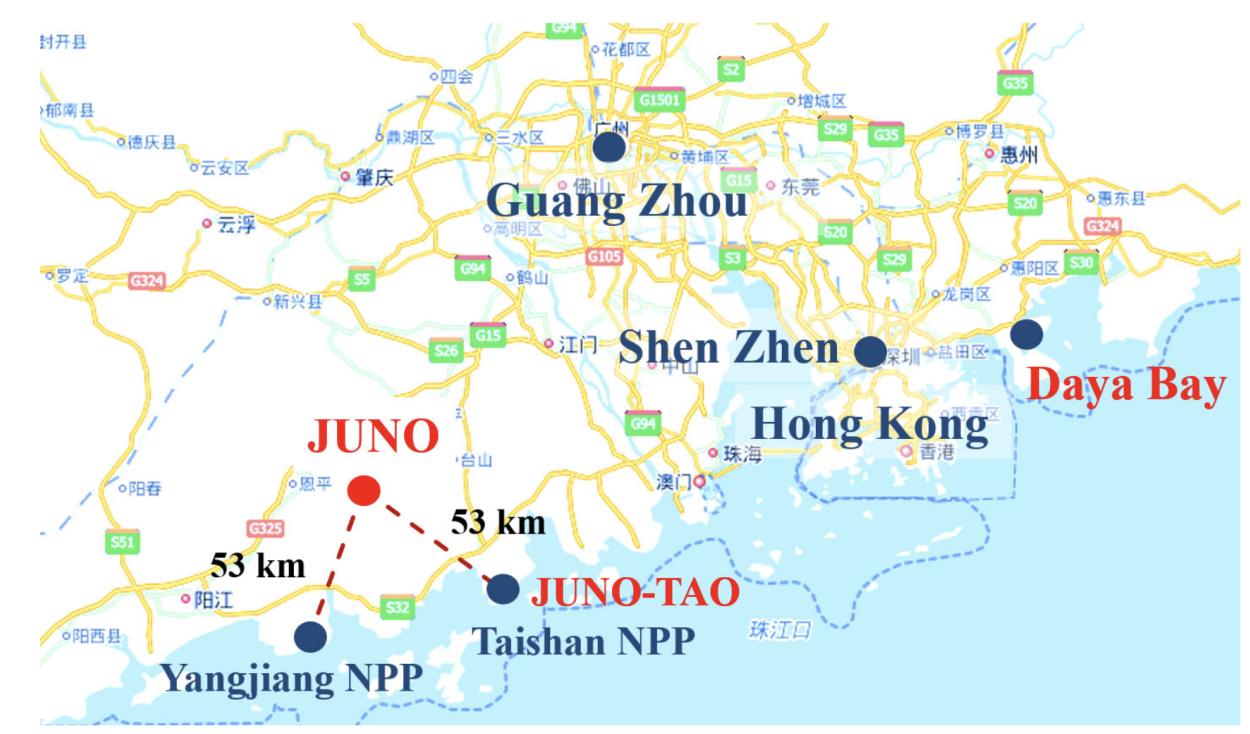
\includegraphics[width=\textwidth]{images/juno/juno_location.png}
  \end{subfigure}
  \hfill
  \begin{subfigure}[b]{0.48\textwidth}
    \centering
    \includegraphics[width=\textwidth]{images/juno/juno_outside.jpg}
  \end{subfigure}
  \caption{\textbf{On the left:} Location of the JUNO experiment and its reactor sources in southern china. \textbf{On the right:} external view of the experimental site}
\end{figure}

For this JUNO will measure the electronic anti-neutrinos ($\bar{\nu}_e$) flux coming from the nuclear reactors of Taishan, Yangjiang, for a total power of 26.6 GW$_{th}$, and the Daya Bay power plant to a lesser extent. Details about the power plants and there expected flux of $\bar{\nu}_e$ can be found in the table \ref{tab:power_plants}.
The distance of 53 km has been specifically chosen to maximize the disappearance probability of the $\bar{\nu}_e$.

\section{Neutrinos physics in JUNO}

\subsection{$\bar{\nu}_e$ flux coming from nuclear power plants}

To get such high measurements precision, it is necessary to have a very good understanding of the source characteristics. For its main studies, JUNO will measure the energy of neutrinos coming from core of nuclear power plants of Taishan and Yangjiang, located at 53 km of the detector to maximise the disappearance probability of the $\bar{\nu}_e$.

\begin{table}[ht]
  \centering
  \begin{tabular}{l c c c c}
    \hline
    Reactor & Power (GW$_{th}$) & Baseline (km) & IBD Rate (day$^{-1}$) & Relative Flux (\%) \\
    \hline
    Taishan    & 9.2  & 52.71 & 15.1 & 32.1 \\
    $~$ Core 1 & 4.6  & 52.77 & 7.5  & 16.0 \\
    $~$ Core 2 & 4.6  & 52.64 & 7.6  & 16.1 \\
    Yangjiang  & 17.4 & 52.46 & 29.0 & 61.5 \\
    $~$ Core 1 & 2.9  & 52.74 & 4.8  & 10.1 \\
    $~$ Core 2 & 2.9  & 52.82 & 4.7  & 10.1 \\
    $~$ Core 3 & 2.9  & 52.41 & 4.8  & 10.3 \\
    $~$ Core 4 & 2.9  & 52.49 & 4.8  & 10.2 \\
    $~$ Core 5 & 2.9  & 52.11 & 4.9  & 10.4 \\
    $~$ Core 6 & 2.9  & 52.19 & 4.9  & 10.4 \\
    Daya Bay   & 17.4 & 215   & 3.0  & 6.4  \\
    \hline
  \end{tabular}
  \caption{Characteristics of the nuclear power plants observed by JUNO. The IBD rate are estimated from the baselines, the reactors full thermal power, selection efficiency and the current knowledge of the oscillation parameters}
  \label{tab:power_plants}
\end{table}

The $\bar{\nu}_e$ coming from reactors are emitted from $\beta$-decay of unstable fission fragments. The Taishan and Yangjiang reactors are pressurised water reactor (PWR), the same type as Daya Bay. In those type of reactor more the 99.7 \% and $\bar{\nu}_e$ are produced by the fissions of four fuel isotopes $^{235}$U, $^{238}$U, $^{239}$Pu and $^{241}$Pu. The neutrino flux per fission of each isotope is determined by the inversion of the measured $\beta$ spectra of fission product \cite{hahn_antineutrino_1989, mueller_improved_2011, von_feilitzsch_experimental_1982, schreckenbach_determination_1985, huber_determination_2011} or by calculation using the nuclear databases \cite{vogel_reactor_1981, dwyer_spectral_2015}. The neutrino flux coming from a reactor at a time $t$ can be predicted using
\begin{equation}
  \phi(E_\nu, t)_r = \frac{W_{th}(t)}{\sum_i f_i(t) e_i} \sum_i f_i(t) S_i(E_\nu)
\end{equation}
where $W_{th}(t)$ is the thermal power of the reactor, $f_i(t)$ is the fraction fission of the $i$th isotope, $e_i$ its thermal energy released in each fission and $S_i(e_\nu)$ the neutrino flux per fission for this isotope. Using this method, the flux uncertainty is expected to be of an order of 2-3 \% \cite{juno_collaboration_sub-percent_2022}.

In addition to those prediction, a satellite experiment named TAO\cite{steiger_tao_2022} will be setup the reactor core Taishan 1 to measure with an energy resolution of 2\% at 1 MeV the neutrino flux coming from the core to identify unknown fine structure and give more insight on the $\bar{\nu}_e$ flux coming from this reactor.

\subsection{Reactor neutrino oscillation for NMO and precise measurements}

Previous works \cite{zhan_determination_2008,  zhan_experimental_2009} shows that oscillation parameters and the NMO can be observed by looking at the $\bnue$ disappearance spectrum coming from medium baseline nuclear reactor. This disappearance probability can be expressed as \cite{an_neutrino_2016} :
\begin{equation*}
  P(\bnue \rightarrow \bnue) = 1 - \sin^2 2\theta_{12} c^4_{13} \sin^2 \frac{\Delta m^2_{21}L}{4E} - \sin^2 2\theta_{13} \bigg[ c_{12}^2 \sin^2 \frac{\Delta m_{31}^2 L}{4E} + s^2_{12} \sin^2 \frac{\Delta m_{32}^2 L}{4E} \bigg]
\end{equation*}
Where $s_{ij} = \sin \theta_{ij}$, $c_{ij} = \cos \theta_{ij}$, $E$ is the $\bnue$ energy and $L$ is the baseline.
We can see the sensitivity to the NMO in the dependency to $\Delta m_{32}^2$ and $\Delta m^2_{31}$ causing a phase shift of the spectrum as we can see in the figure \ref{fig:juno-spectrum-oscillation}.
By carefully fitting this spectrum, one can extract the NMO and the oscillation parameters. The fit is reviewed in more details in the section \ref{sec:Fit}

\begin{figure}
  \centering
  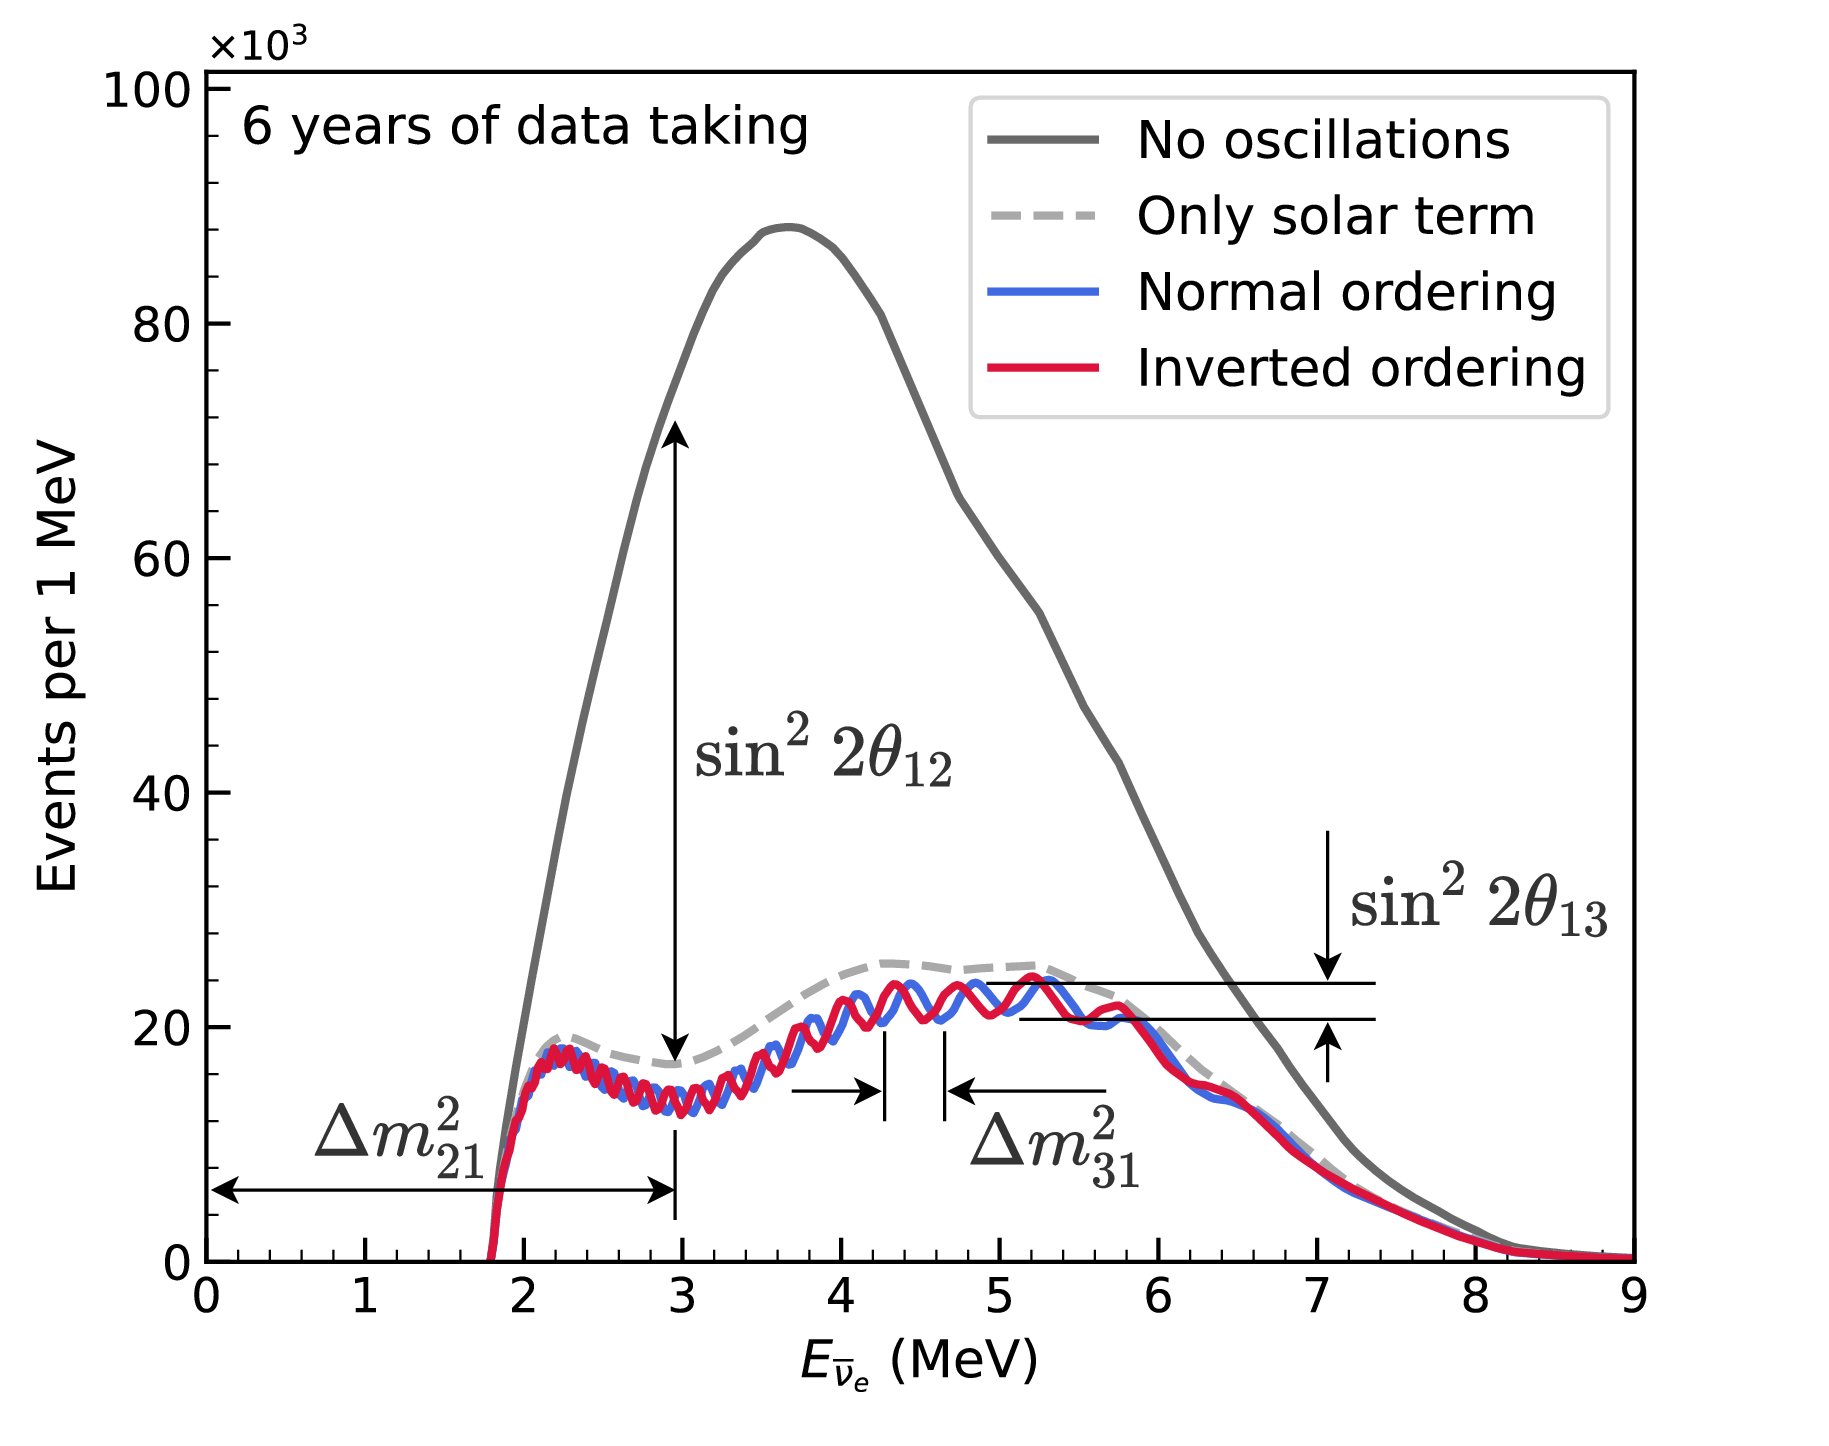
\includegraphics[height=8cm]{images/juno/Spectrum-OscillationsOnly_dm2_31.png}
  \caption{Expected number of neutrinos event per MeV in JUNO after 6 years of data taking. The black curve shows the flux if there was no oscillation. The light gray curve shows the oscillation if only the solar terms are taken in account ($\theta_{12}$, $\Delta m_{21}^2$). The blue and red curve shows the spectrum in the case of, respectively, NO and IO. The dependency of the oscillation to the different parameters are schematized by the double sided arrows. We can see the NMO sensitivity by looking at the fine phase shift between the red and the blue curve.}
  \label{fig:juno-spectrum-oscillation}
\end{figure}

To reach the desired sensitivity, JUNO must meet multiple requirements but most notably:
\begin{enumerate}
  \item An energy resolution of $3\%/\sqrt{E\mathrm{(MeV)}}$ to be able to distinguish the fine structure of the fast oscillation.
  \item An energy precision of 1\% in order to not err on the location of the oscillation pattern.
  \item A baseline of 53 $\pm$ 0.5 km to maximise the $\bar{\nu}_e$ oscillation probability.
  \item At least $\approx$ 100,000 events to limit the spectrum distortion dur to statistical uncertainties.
\end{enumerate}

\subsubsection{Identification of the mass ordering}

To identify the mass ordering, we fit the neutrino energy spectrum under the two hypothesis of NO and IO. Those two fit give us two $\chi^2$, respectively $\chi^2_{NO}$ and $\chi^2_{IO}$. By computing the difference $\Delta \chi ^2 = \chi^2_{NO} - \chi^2_{IO}$ we can determine the most probable mass ordering: NO if $\Delta \chi^2 > 0$ and IO if $\Delta \chi^2 < 0$. Current studies shows that the expected sensitivity the mass ordering would be of $3.4 \sigma$ after 6 years of data taking in nominal setup\cite{an_neutrino_2016}. More detailed explanations about the fitting procedure can be found in the section \ref{sec:Fit}.

\subsubsection{Precise measurement of the oscillations parameters}

The oscillations parameters $\theta_{12}$, $\theta_{13}$, $\Delta m^2_{21}$, $\Delta m^2_{31}$ are free parameters in the fit of the oscillation spectrum. The precision on those parameters have been estimated and are shown in figure \ref{fig:juno-param-precision}. Wee see that for $\theta_{12}$, $\Delta m^2_{21}$, $\Delta m^2_{31}$, precision at 6 years is better than the reference precision by an order of magnitude \cite{juno_collaboration_sub-percent_2022}

\begin{figure}[hb]
  \centering
  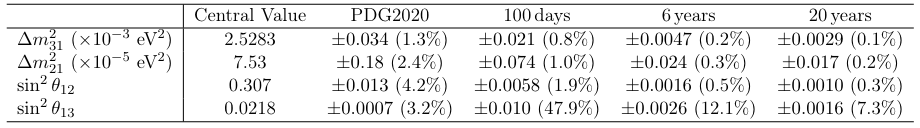
\includegraphics[width=\linewidth]{images/juno/oscillation_params_precision.png}
  \caption{A summary of precision levels fir the oscillation parameters. The reference value (PDG 2020 \cite{particle_data_group_review_2020}) is compared with 100 days, 6 years and 20 years of JUNO data taking.}
  \label{fig:juno-param-precision}
\end{figure}

\subsection{Other physics}

While the design of JUNO is tailored to measure $\bar{\nu}_e$ coming from nuclear reactor, JUNO will be able to detect neutrinos coming from other sources thus allowing for a wide range of physics studies as detailed in the table \ref{tab:signal} and in the following sub-section.

\begin{table}[ht]
\begin{center}
  \begin{tabular}{|c|c|c|c|}
    \hline Research & Expected signal & Energy region & Major backgrounds \\
    \hline Reactor antineutrino & 60 IBDs/day & 0–12 MeV  & Radioactivity, cosmic muon \\
    Supernova burst & 5000 IBDs at 10 kpc & 0–80 MeV & Negligible \\
                    & 2300 elastic scattering  & &  \\
    DSNB (w/o PSD) & 2–4 IBDs/year & 10–40 MeV & Atmospheric $\nu$ \\
    Solar neutrino & hundreds per year for $^8$B & 0–16 MeV & Radioactivity \\
    Atmospheric neutrino & hundreds per year & 0.1–100 GeV  & Negligible \\
    Geoneutrino &  $\approx 400$ per year & 0–3 MeV & Reactor $\nu$ \\
    \hline
  \end{tabular}
  \caption{Detectable neutrino signal in JUNO and the expected signal rates and major background sources}
  \label{tab:signal}
\end{center}
\end{table}


\subsubsection{Geoneutrinos}

Geoneutrinos designate the antineutrinos coming from the decay of long-lived radioactive elements inside the Earth. The 1.8 MeV threshold necessary for the IBD makes it possible to measure geoneutrinos from $^238$U and $^232$Th decay chains. The studies of geoneutrinos can help refine the Earth crust models but is also necessary to characterise their signal, as they are a background to the mass ordering and oscillations parameters studies.

\subsubsection{Atmospheric neutrinos}

Atmospheric neutrinos are neutrinos originating from the decay of $\pi$ and $K$ particles that are produced in extensive air showers initiated by the interactions of cosmic rays with the Earth atmosphere. Earth is mostly transparent to neutrinos below the PeV energy, thus JUNO will be able to see neutrinos coming from all directions. Their baseline range is large (15km $\sim$ 13000km), they can have energy between 0.1 GeV and 10 TeV and will contain all neutrino and antineutrinos flavour. Their studies is complementary to the reactor antineutrinos and can bring constraint on the MO \cite{an_neutrino_2016}.

\subsubsection{Beyond standard model neutrinos interactions}

JUNO will also be able to probe for beyond standard model neutrinos interactions. After that the main physics topics have been accomplished, JUNO could be upgraded to probe for neutrinoless beta decay ($0\nu\beta\beta$). The detection of such event would give critical informations about the nature of neutrinos, is it a majorana or a dirac particle. JUNO will also be able to probe for neutrinos that would come for the decay or annihilation of Dark Matter inside the sun and neutrinos from putative primordial black hole.
Through the unitary test of the mixing matrix, JUNO will be able to search for light sterile neutrinos.
Thanks to JUNO sensitivity, multiple other exotic can be performed on neutrino related beyond standard model interactions.

\subsubsection{Supernovae burst neutrinos}

Neutrinos are crucial component during all stages of stellar collapse and explosion. Detection of neutrinos coming for core collapse supernovae will provide us important informations on the mechanisms at play in those events.
Thanks to its 20 kt LS, JUNO has excellent capabilities to detect all flavour of the $\mathcal{O}$(10 MeV) postshock neutrinos, and using neutrinos of the $\mathcal{O}$(1 MeV) will give informations about the pre-supernovae neutrinos. All those informations will allow to disentangle between the multiple hydro-dynamic models that are currently used to describe the different stage of the core-collapse.

\subsubsection{Diffuse supernovae neutrinos background}

Core-collapse supernovae in our galaxy are rare events, but they frequently occur throughout the visible Universe sending burst of neutrinos in direction of the Earth. All those events contributes to a low background flux of low-energy neutrinos called the Diffuse Supernovae Neutrino Background (DSNB). Its flux and spectrum contains informations about the red-shift dependent supernovae rate, the average SN neutrino energy and the fraction of black-hole formation in core-collapse supernovae. Depending of the DSNB model, we can expect 2-4 IBD events per year in the energy range above the reactor $\bar{\nu}_e$ signal, which is competitive with the current Super-Kamiokande+Gadolinium phase.

\subsubsection{Background in the neutrinos reactor spectrum}

Considering the close reactor neutrinos flux as the main signal, the signals that are considered as background are:
\begin{itemize}
  \item The geoneutrinos producing background in the 0.511 $\sim$ 2.7 MeV region.
  \item The neutrinos coming from the other nuclear reactors around Earth.
\end{itemize}
In addition to all those physics signal, non-neutrinos signal that would mimic an IBD will also be present. It is composed of:
\begin{itemize}
  \item The signal coming from radioactive decay ($\alpha, ~ \gamma, ~ \beta$) from natural radioactive isotopes in the material of the detector.
  \item Cosmogenic event such as fast neutrons and activated isotopes induced by muons passing through the detector, most notably the spallation on $^12$C.
\end{itemize}
All those events represent a non-negligeable part of the spectrum as shown in figure \ref{fig:spectrum_with_background}.

\begin{figure}[ht]
  \centering
  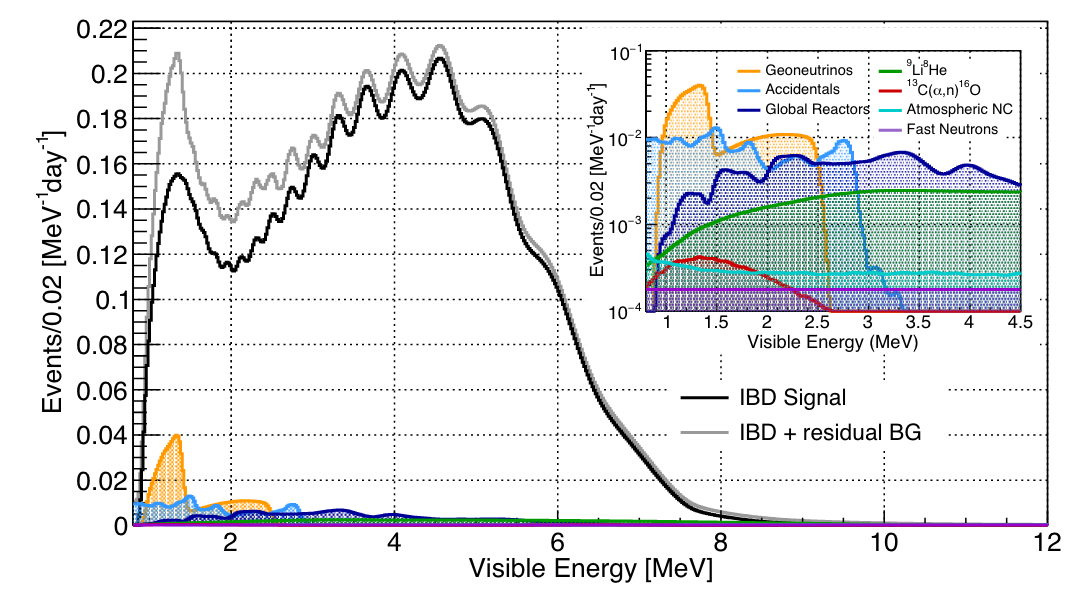
\includegraphics[height=6cm]{images/juno/spectrum_with_background.png}
  \caption{Expected visible energy spectrum measured with the LPMT system with (grey) and without (black) backgrounds. The background amount for about 7\% of the IBD candidate and are mostly localized below 3 MeV \cite{juno_collaboration_sub-percent_2022}}
  \label{fig:spectrum_with_background}
\end{figure}


\section{The JUNO detector}

\todo{1. Expliquer "grossierement" le detecteur, 2. Mettre ici toutes informations qui ne rentrerait pas dans les section suivantes (aka overburden, etc...)}

\subsection{Principle of detection}

JUNO will be able to detect neutrinos and measure their energy mainly via the Inverse Beta Decay (IBD) interaction
\begin{equation*}
  \bar{\nu}_e + p \rightarrow n + e^+
\end{equation*}
Simple kinematics calculation shows that the $\bar{\nu}_e$ must have an energy of $ (m_n + m_e - m_p ) \approx 1.806 ~ \mathrm{MeV}$ \cite{strumia_precise_2003} where $m_\lambda$ is the mass of the $\lambda$ particle.
This threshold make the experiment blind to very low energy neutrinos. The residual energy $E_{\nu} - 1.806 ~ \mathrm{MeV}$ is be distributed as kinetic energy between the positron and the neutron.
The energy of the emitted positron $E_e$ is given by \cite{strumia_precise_2003}
\begin{equation}
  E_e = \frac{(E_\nu - \delta)(1+\epsilon_\nu) + \epsilon_\nu \cos \theta \sqrt{(E_\nu - \delta)^2 + \kappa m_e^2}}{\kappa}
\end{equation}
where $\kappa = (1 + \epsilon_\nu)^2 - \epsilon_\nu^2 \cos^2 \theta \approx 1$, $\epsilon_\nu = \frac{E_\nu}{m_p} \ll 1$ and $\delta = \frac{m_n^2 - m_p^2 - m_e^2}{2m_p} \ll 1$.
We can see from this equation that the positron energy is strongly correlated to the neutrino energy.

Once the positron and the neutron will propagate in the detection medium, the liquid scintillator (LS), loosing their kinetic energy by exciting with the LS. Once stopped, the positron will annihilate with an electron from the medium producing two 511 KeV gamma. Those gamma will themselves interact with the LS, exciting it before being absorbed by photoelectrical effect. The neutron will be captured by an hydrogen, emitting a 2.2 MeV gamma in the process. This gamma will also deposit its energy before being absorbed by the LS.

\begin{figure}[ht]
  \centering
  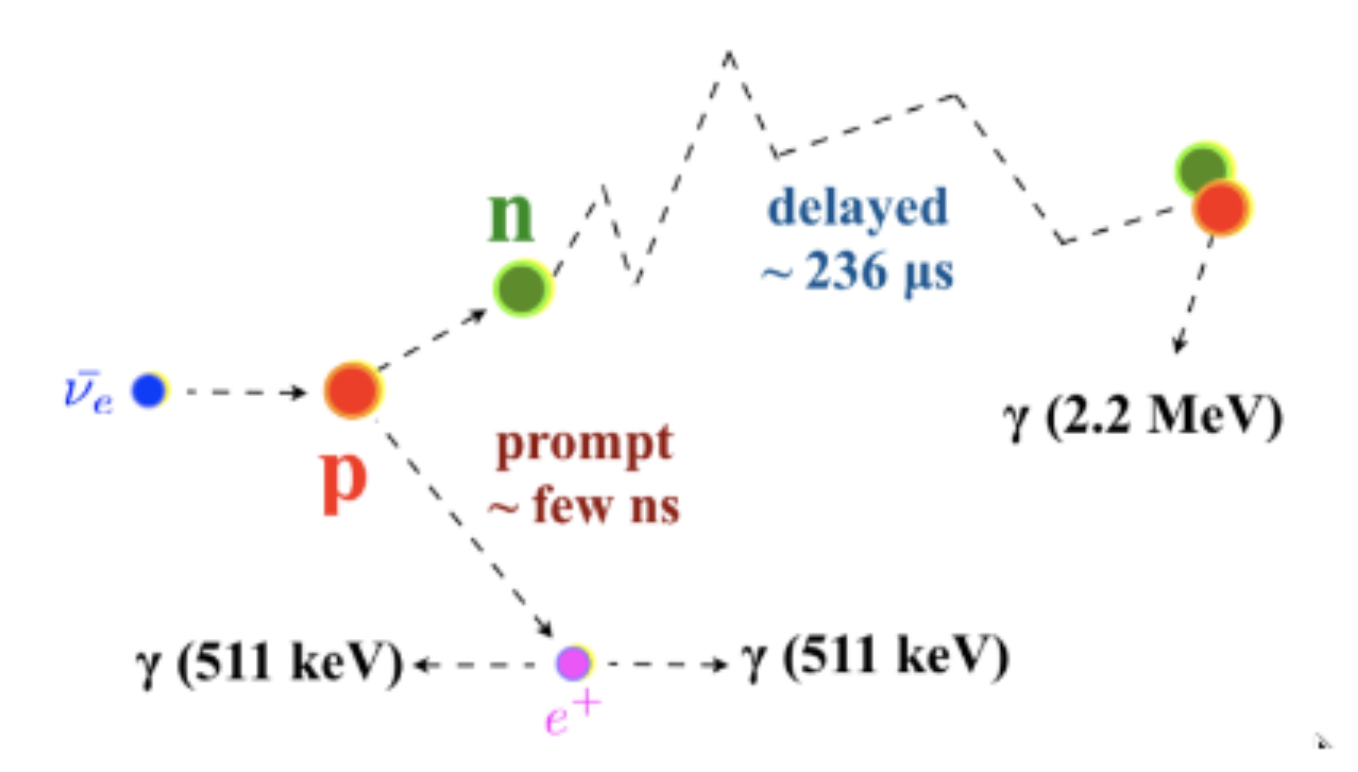
\includegraphics[width=8cm]{images/juno/IDB-JUNO.png}
  \caption{Schematics of an IBD interaction in the central detector of JUNO}
  \label{fig:IBD}
\end{figure}

More details about the LS can be found in section \ref{sec:CD}.

The scintillation photons will then be captured by the photo-multipliers (PMTs) surrounding the experiment. The analogue signal, then digitized by the electronic is the signal of our experiment. The signal produced by the positron is subsequently called the prompt signal, and the signal coming from the neutron the delayed signal. This naming convention come from the fact that the positron will deposit its energy rather quickly (few ns) where the neutron will take a bit more time ($\sim$ 236 $\mu$s).

\subsection{Central Detector (CD)}
\label{sec:CD}

\subsubsection{Acrylic containment sphere}

\subsubsection{Liquid scintillator}

\subsubsection{Large photo-multipliers (LPMTs)}

\subsubsection{Small photo-multipliers (SPMTs)}

\subsubsection{Data Acquisition System (DAQ)}

\subsubsection{Simulation}

\subsubsection{Software}

\todo{Expliquer comment le software fonctionne}


\subsection{Veto detector}

\subsubsection{Cherenkov in water pool}

\subsubsection{Top tracker}

\section{Calibration strategy}

\subsection{Energy scale calibration}

\subsection{Calibration system}

\subsection{Calibration program}

\section{Event selection and background rejection}

\todo{Explication de comment reconnaitre un IDB (OEC)}

\subsection{Fiducial volume}

\subsection{Muon tagging}

\section{State of the art of the IBD reconstruction}

\subsection{Interaction vertex reconstruction}

\subsection{Energy reconstruction}

\subsection{Particle identification}

\subsection{Machine learning for reconstruction}

\subsubsection{Vertex reconstruction}

\subsubsection{Energy reconstruction}

\section{JUNO sensitivity to NMO and precise measurements}

\subsection{Fitting procedure}
\label{sec:Fit}


\documentclass[../main.tex]{subfiles}
\graphicspath{{\subfix{..}}}

\begin{document}
\chapter{Introduction to the reconstruction methods and algorithms used in this thesis}
\label{sec:ml}

\epigraph{``I have the shape of a human being and organs equivalent to those of a human being. My organs, in fact, are identical to some of those in a prosthetized human being. I have contributed artistically, literally, and scientifically to human culture as much as any human being now alive. What more can one ask?''}{Isaac Asimov, The Complete Robot}

\minitoc

Machine Learning (ML) and more specifically Neural Network (NN) are families of data-driven algorithms. They are used in a wide variety of domains including natural language processing, computer vision, speech recognition and, the subject of this thesis, scientific studies.

Machine learning models aim to learn underlying patterns from finite datasets in order to make general predictions or classifications.
For example, in our case, it could be an algorithm that would differentiate the nature of a particle interacting in the liquid scintillator, between a positron and an electron, based on the readout charge and time $(Q, t)$ of the 17612 LPMT of the JUNO experiment. During a first training phase, it would learn the discriminative features between the two in the 35224-dimensional charge and time distribution, built from samples of $e^+$ and $e^-$ events.

It extracts essential features from a highly complex and multi-dimensional dataset that describe the physical interactions: a three body energy deposition (the positron and two annihilation gammas) and the single deposit from an electron.

Ideally, the algorithm would learn to recognize those informations on its own, regardless of the input size and complexity. In practice, however, these algorithms are guided by human design through their architectures and training conditions. We can still hope that they an use more thoroughly the detector informations while traditional methods are often subject to assumptions or simplifications to make the task easier (see for instance the algorithm in Section \ref{sec:juno:reco}).

The role of machine learning algorithms has expanded rapidly in the past decade, either as the main or secondary algorithm for a wide variety of tasks: event reconstruction, event classification, waveform reconstruction and so on. In particular in domains where the underlying physic and detector processes are complex and highly dimensional, and when large amount of data must be processed quickly.

This chapter present an overview of the different kind of machine learning methods and neural networks that will be discussed in this thesis, and the state of the art of the reconstructions methods in JUNO our ML algorithms will be compared to.

\section{Core concepts in machine learning and neural networks}

In this section, we discuss the core concepts in machine learning that will be used thorough this thesis. We place particular emphasis on Neural Networks, as it's the family of the algorithms described in chapters \ref{sec:jcnn}, \ref{sec:jgnn} and \ref{sec:janne}.

\subsection{Boosted Decision Tree (BDT)}
\label{sec:ml:bdt}

One of the most classic machine learning algorithm used in particle physics is Boosted Decision Tree (BDT) \cite{breiman_classification_2017} (or more recently Gradient Boosting Machine \cite{friedman_greedy_2001}).

BDTs operate by making a series of decisions based on a set of input features, with each decision represented as a node in the tree.
Each decision point, or node, takes its decision based on a set of trainable parameters leading to a subtree of decisions. The process is repeated until it reach the final node, yielding the prediction. A simplistic example is given in Figure \ref{fig:ml:bdt}.

\begin{figure}
  \centering
  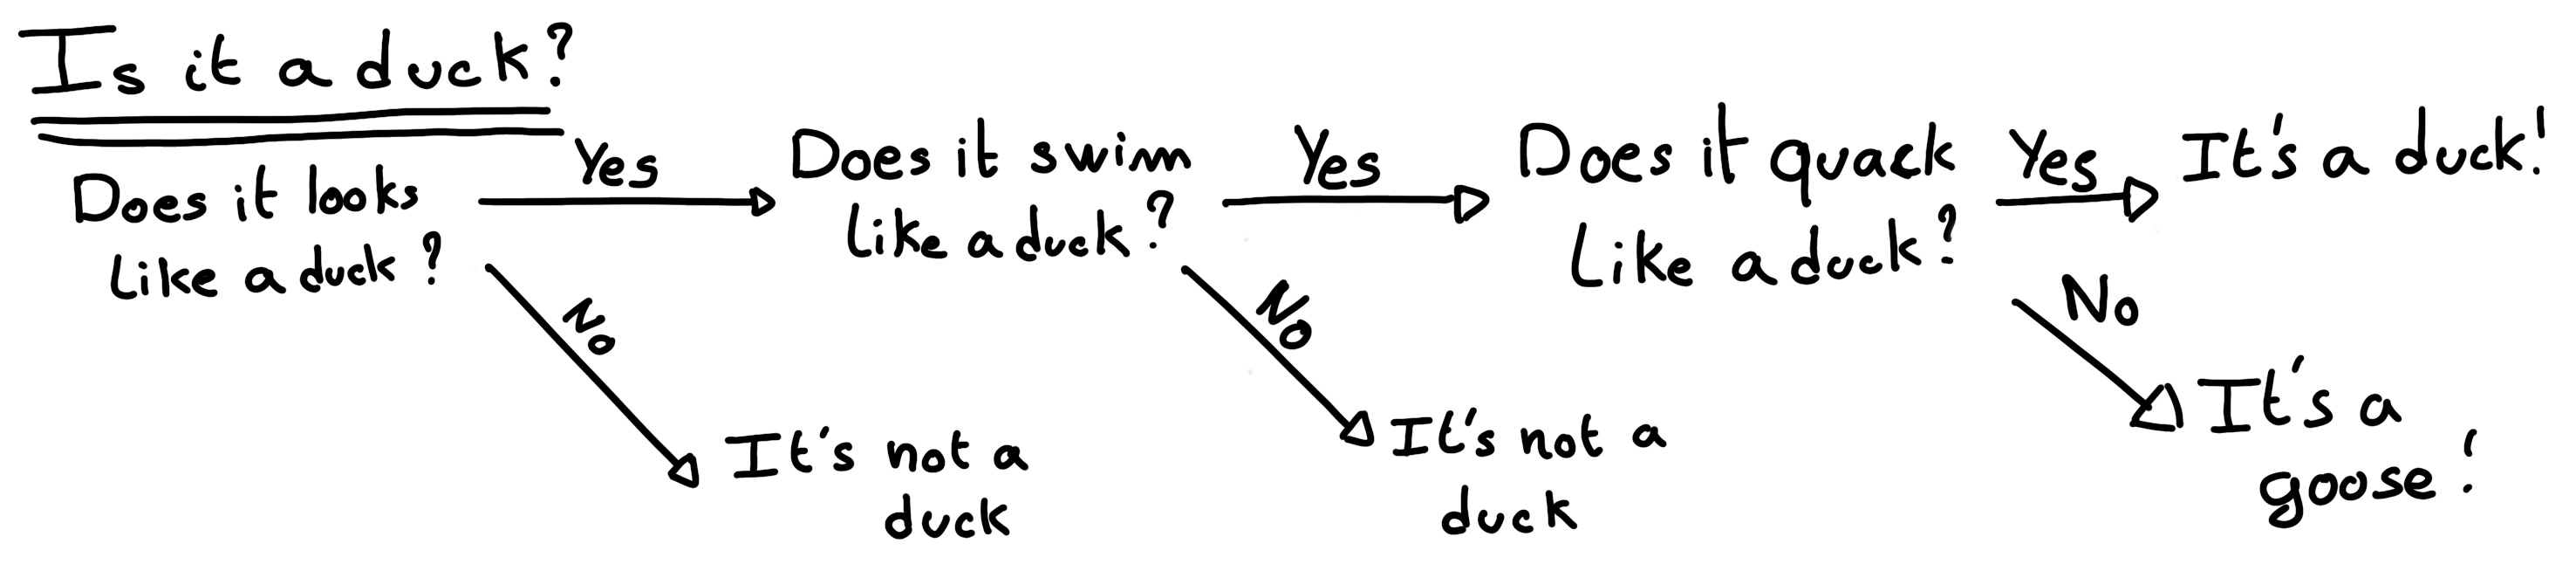
\includegraphics[width=\linewidth]{images/ml/Bdt.jpg}
  \caption{Example of a BDT that determine if the given object is a duck}
  \label{fig:ml:bdt}
\end{figure}

The training procedure followes a reward-based approach where the algorithm predictions are compared to the true outcomes.
During the training phase the prediction of the BDT is compared to a known truth about the data. The score is then used to backpropagate corrections to the parameters of the tree. Modern BDT use gradient boosting where the gradient of the loss is calculated for each of the BDT parameters. Following the gradient descent, we can reach the, hopefully, global minima of the loss for our set of parameters.

\subsection{Artificial Neural Network (NN)}
\label{sec:ml:nn}

One of the modern ML family is the Neural Network, historical name as their design was inspired by the behaviour of biological neurons in the brain.
\begin{figure}[ht]
  \centering
  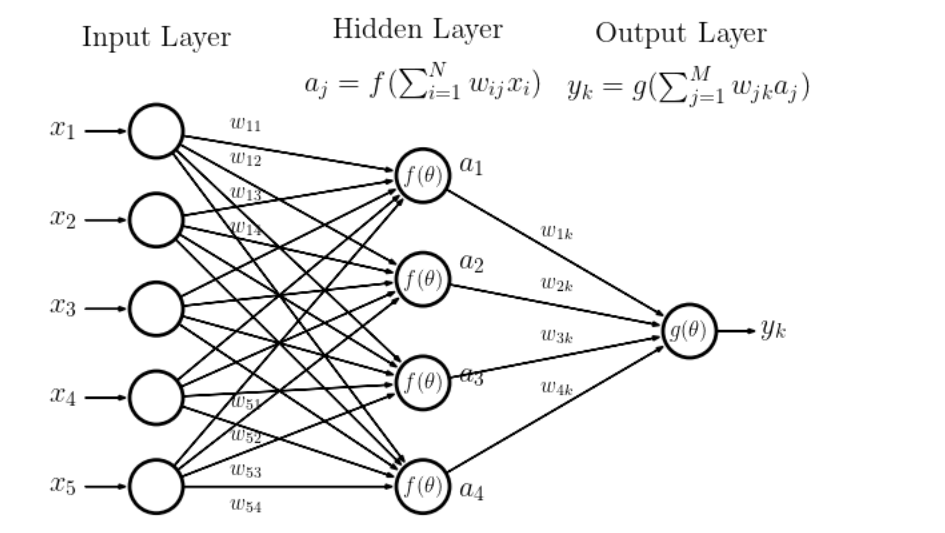
\includegraphics[height=6cm]{images/ml/nn_explications.png}
  \caption{Schema of a simple neural network}
  \label{fig:ml:schema_nn}
\end{figure}
As schematized in Figure \ref{fig:ml:schema_nn}, the input, output and steps inside the NN is described as neuron \textit{layers}. The neurons of the layers take as input a set of values from the preceding layer, here the $a_i$ takes every informations of the $x_i$ input layer, and aggregate those values following learnable \textit{parameters} $w_{ij}$. In the example in Figure \ref{fig:ml:schema_nn}, fully connected layers are used, meaning that each neuron in one layer is connected to every neuron in the previous layer.

The aggregation procedure is core of defining the architecture of the NN. The different architectures used in this thesis will be discussed in Section \ref{sec:ml:architecture}. The process is repeated until reaching the output layer.

For example, let's take the network in Figure \ref{fig:ml:schema_nn} and say that $a_1$, $a_2$ and $a_3$ are the neurons of the output layer. We try to produce a vertex reconstruction algorithm that will approach the charge barycentre. Let's limit the input $x_i$ to the charge of the $i$th PMT, one of the solution is to aggregate on $a_1$ the $x$ coordinate of the barycenter. The network would thus adapt the $w_{i1}$ parameters so they correspond to the $x$ coordinates of the $i$th PMT. Same for the $y$ and $z$ coordinate on $a_2$ and $a_3$ respectively.

The layers used in the example above are designated as \textit{Fully connected} layers, where every neurons of the layer is connected to the every neurons of the preceding layer. The layer can be expressed using the Einstein summation and in bold the learnable parameters
\begin{equation}
  \label{eq:ml:fully-connected-simple}
  O_{j} = I_{i} + \bm{W}_{j}^{i}
\end{equation}
where $O_{j}$ is the output neurons vector (the $a_i$), $I_{i}$ is the preceding layer neurons vector (the $x_i$) and $\bm{W}$ is the parameters, or weights, matrix (composed of the $w_{ij}$).
In practice, this fully connected layer is often adjoined a bias $\bm{B}$ and an \textit{activation function} $F$.
\begin{equation}
  \label{eq:ml:fully-connected}
  I_{j} = F(I_{i} \bm{W}_{j}^{i} + \bm{B}_j)
\end{equation}

This is the fundamental component of the Fully Connected Deep NN (FCDNN) family presented in Section \ref{sec:ml:fcdnn}.

This description of neural networks as layers introduce the principles of \textit{depth} and \textit{width}, the number of layers in the NN and the number of neurons in each layer respectively. Those quantities that not directly used for the computation of the results but describes the NN or its training are designated as \textit{hyperparameters}.

Now we just need to adapt the parameters so that this network learn that $w_{ij}$ are the PMT coordinate. We describe the space produced by the parameters of the network as the \textit{parameter phase space} or \textit{latent space}. The optimization of the network and exploration of this phase space is done through training over a \textit{training dataset} as described in next section.

\subsection{Training procedure}
\label{sec:ml:train}

To adapt the parameters we need an object that describe how well the network perform. This is the \textit{loss} of our neural networks $\mathcal{L}$. In our barycenter example, it could be the distance between the reconstructed and real barycenter. Using this metric we can adjust the parameters of our network.

Depending if we try to minimize or maximize it, it need to posses a minima or a maxima. For example when doing \textit{regression}, i.e. produce a scalar result like the coordinates of a barycenter, a common loss is the Mean Square Error (MSE). Let $i$ be our dataset, the $N$ events considered for training, $y_i$ be the target scalar, the barycenter positions of each events, $x_i$ the input data, the charge vector, and $f(x_i, \bm{\theta})$ the result of the network. The network here is modelled by $f$, and its parameter $\bm{\theta}$
\begin{equation}
  \mathcal{L} \equiv MSE = \frac{1}{N} \sum_i^N (y_i - f(x_i, \bm{\theta}))^2
\end{equation}
Another common loss function is the Mean Absolute Error (MAE)
\begin{equation}
  \mathcal{L} \equiv MAE = \frac{1}{N} \sum_i^N |y_i - f(x_i, \bm{\theta})|
\end{equation}

We see that those loss function possess a minima when $f(x_i, \bm{\theta}) = y_i$.


Modern neural networks typically use gradient descent to optimize their parameters by minimizing the loss function. The gradient of the parameter $\bm{w}$, designated in literature as $\bm{\theta}$, with respect to the loss function $\mathcal{L}$ is subtracted each optimisation step $t$
\begin{equation}
  \bm{\theta}_{t+1} = \bm{\theta}_t - \frac{\partial \mathcal{L}}{\partial \bm{\theta}}
\end{equation}
This induce $\mathcal{L}$  needs to be differentiable with respect to $\bm{\theta}$, thus the layers and their activation functions also need to be differentiable. This simple gradient descent, designated as Stochastic Gradient Descent (SGD), can be extended with first and second order momentums like in the Adam optimizer \cite{kingma_adam_2017}. More details about the optimizers can be found in Section \ref{sec:ml:optim}.

\subsubsection{Training lifecycle}

The training process of neural networks can vary depending on the application and dataset, but in this thesis, we follow a standard approach. As shown in Fig. \ref{fig:ml:lifecycle}, training is organized into \textit{epochs}, each of which consists of several \textit{steps}. During each step, the neural network optimizes its parameters using a \textit{batch}, a subset of the entire training dataset.

\begin{figure}[ht]
  \centering
  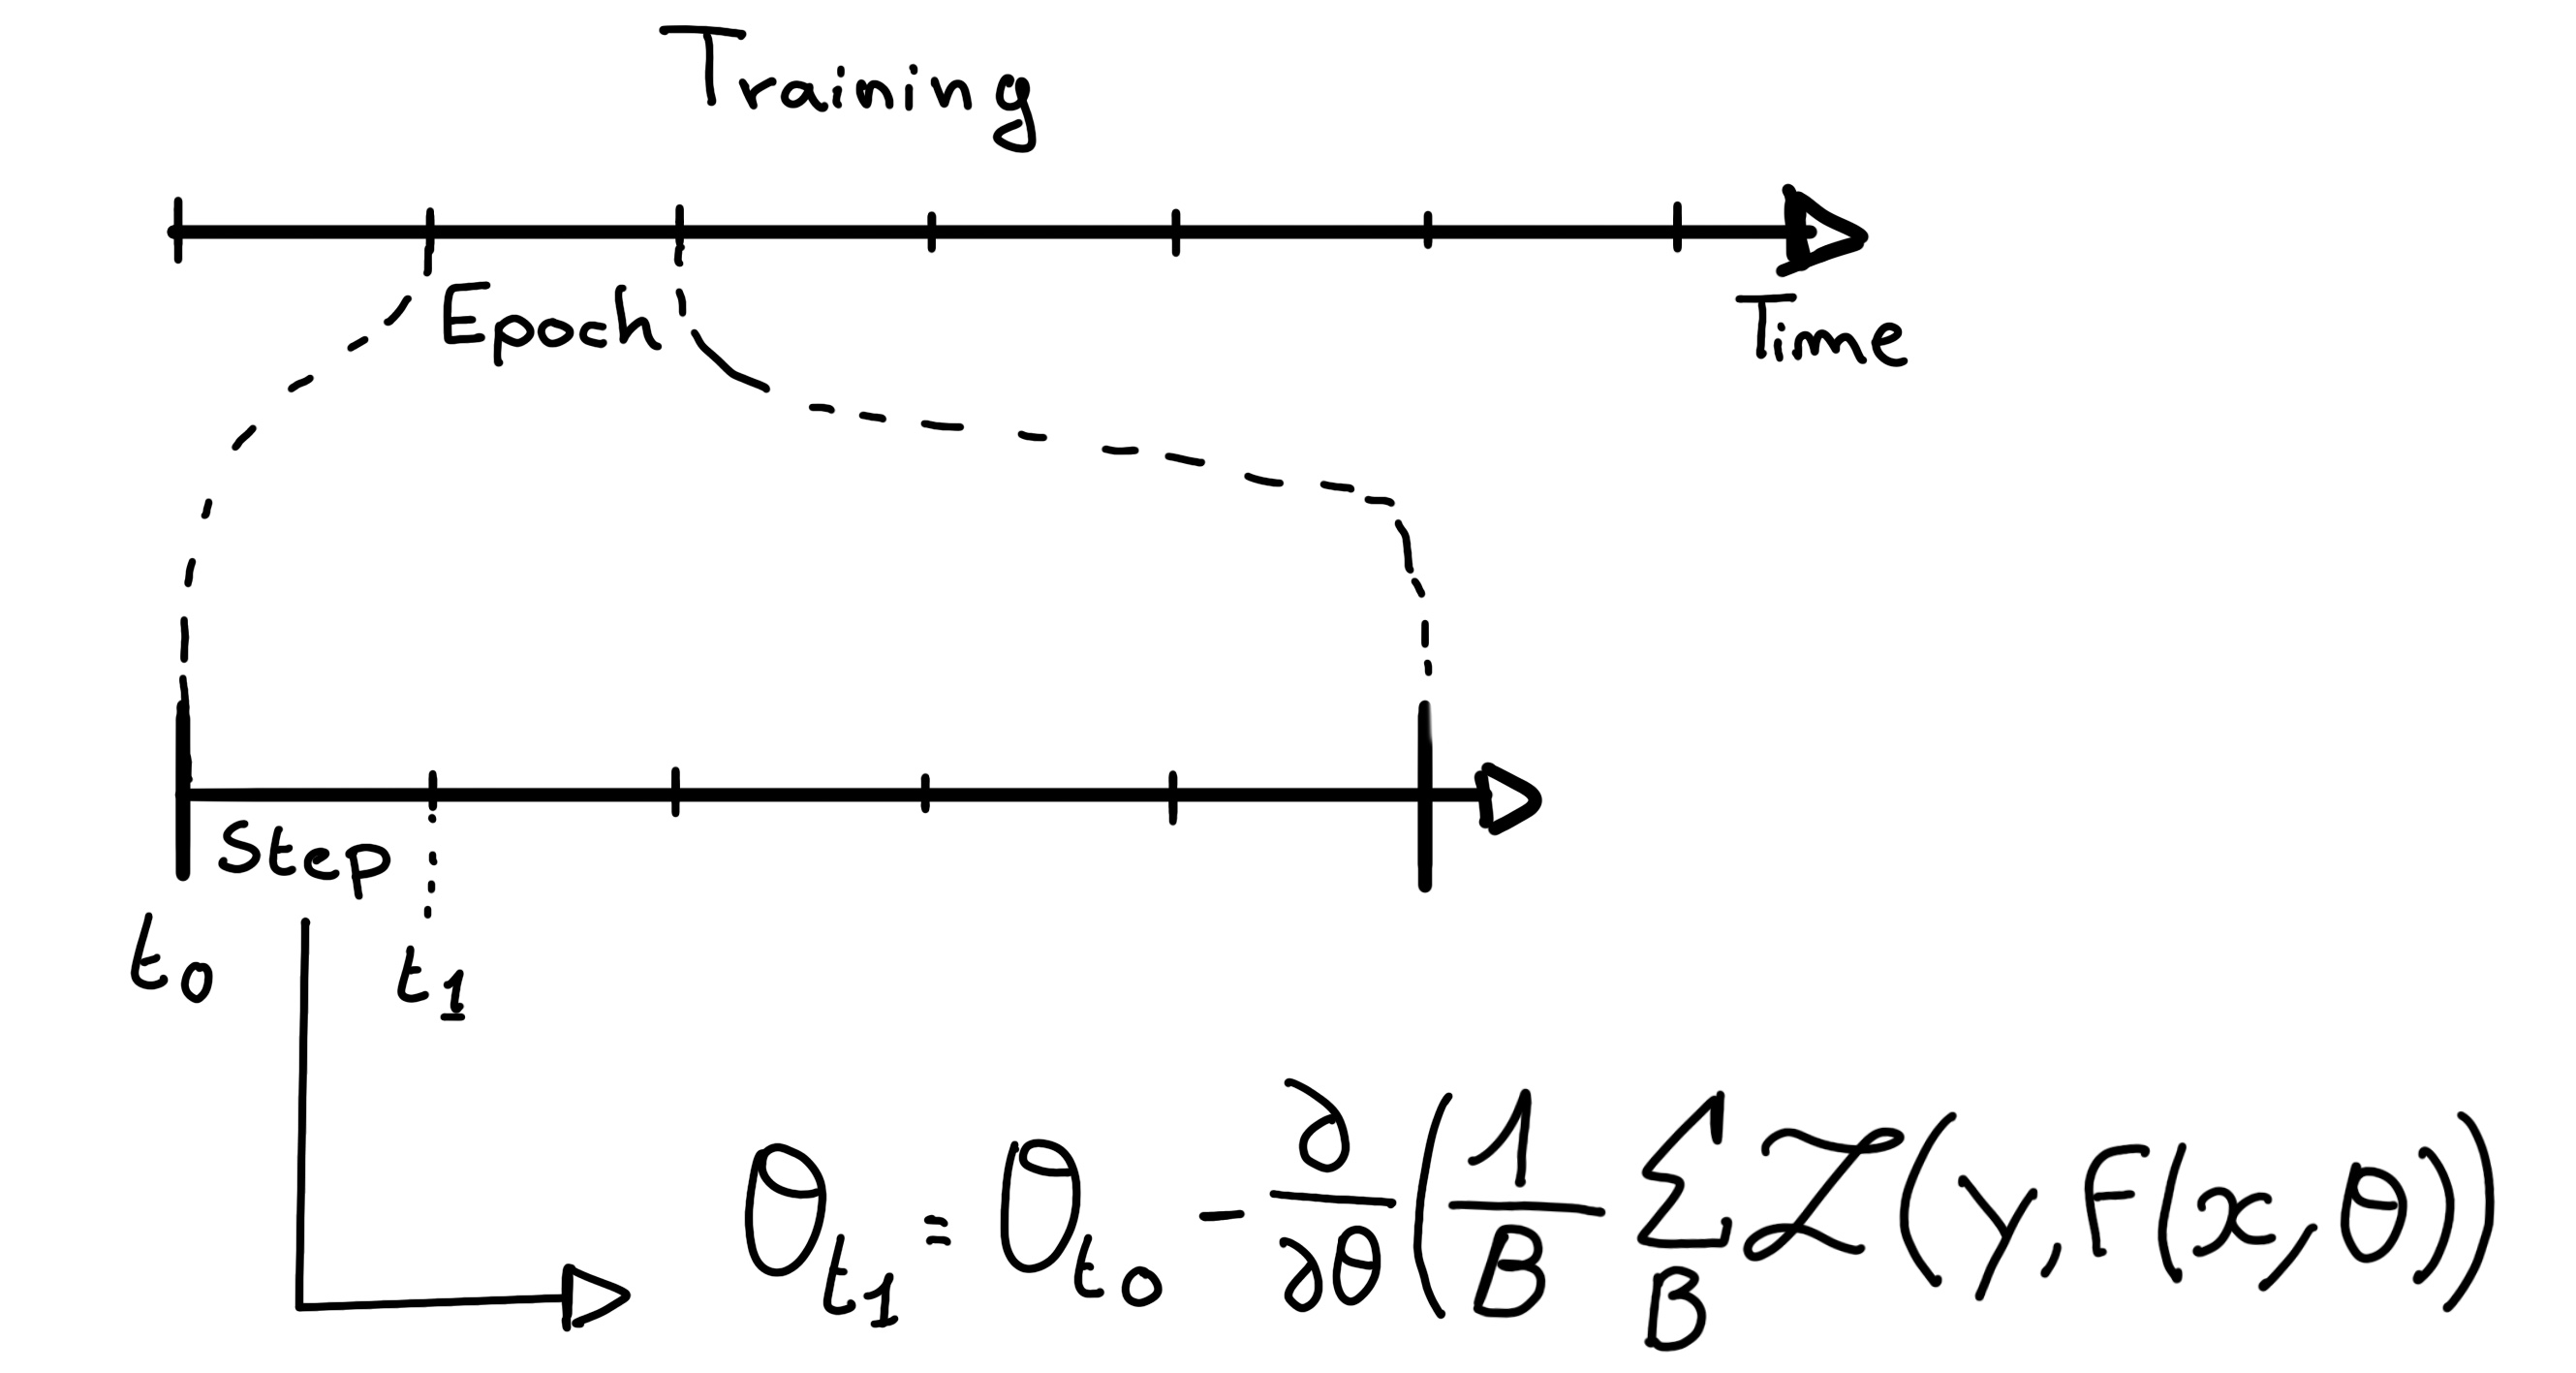
\includegraphics[height=6cm]{images/ml/lifecycle.jpg}
  \caption{Illustration of the training lifecycle}
  \label{fig:ml:lifecycle}
\end{figure}

The ideal batch size vary depending of the problematic, as it has been shown that too big of a batch size could lead to the network being stuck in local minima, while too small batch size tend to lead to noisy reponse from the netowrk. Moreover, in our case, we are limited by the memory consumption as our dataset, or even to big batches, might not fully fit in memory.

At the end of each epoch, the neural network is evaluated on a validation dataset, which is not used during training. This dataset serves as a reference to assess the network's performance and avoid potential pitfalls such as overfitting. Those pitfalls will be further discussed in Section \ref{sec:ml:pitfall}. In JUNO, this is critical because the model needs to generalize well to unseen experimental data and avoid focussing on noise in the training dataset.

Hyperparameters that can be optimized during the training can be optimized at each epoch, for example the learning rate, or each step, the optimizer momentum for example.

There is not really a typical number of epochs or steps for the training. The number steps can be defined such as in one epoch, the NN see the entirety of the dataset but the number of steps and epochs are hyperparameters that are optimized over the each subsequent training. We adjust them by looking at the loss evolution profile over time.

Most training are started with a fixed number of epochs, i.e. from what we've seen from precedent training, the network stop learning, the loss is constant, after $N$ epoch so we run the training for $N+\delta$ epochs to see if the modification brings improvements to the loss profile.
We can implement \textit{early stopping policies} to halt training if certain conditions are met, such as a sudden increase in loss or when the loss plateaus. However, for the JUNO experiment, where training time is not a strict limitation, early stopping is less critical, though it may still be useful to prevent overfitting in some cases

\subsubsection{The optimizer}
\label{sec:ml:optim}

As briefly introduced at the beginning of this section, the parameters of the neural network are optimized using the gradient descent method. We compute the gradient of the mean loss over the batch with respect to each parameters and we update the parameters in accord to minimize the loss. The  gradient is computed backward from the loss up to the first layer parameters using the chain rule, in this case with only one parameter at each step for simplicity:
\begin{equation}
  \label{eq:ml:backward}
  \frac{\partial \mathcal{L}}{\partial \theta_1} = \frac{\partial \theta_2}{\partial \theta_1} \frac{\partial \mathcal{L}}{\partial \theta_2} = \frac{\partial \theta_2}{\partial \theta_1} \frac{\partial \theta_3}{\partial \theta_2} \frac{\partial \mathcal{L}}{\partial \theta_3} = \frac{\partial \theta_2}{\partial \theta_1} \prod_{i=2}^{N-1} \frac{\partial \theta_{i+1}}{\partial \theta_i} \frac{\partial \mathcal{L}}{\partial \theta_N}
\end{equation}
where $\theta$ is a parameter, $i$ is the layer index. We see here that the gradient of the first layer is dependent of the gradient of all the following layers. Because the only value known at the start of the optimization procedure is $\mathcal{L}$ we compute $\frac{\partial \mathcal{L}}{\partial \theta_N}$ then, $\frac{\partial \theta_{N}}{\partial \theta_{N-1}}$, etc... This is called the \textit{backward propagation}.

This update of the parameters is done following an optimizer policy. Those optimizers depends on hyperparameters. The ones used in this thesis are:

\begin{enumerate}
  \item Stochastic Gradient Descent (SGD).
    A simple but widely used optimizer that relies on one key hyperparameter, the learning rate (LR) / $\lambda$. It update each step the parameters $\theta$ following
    \begin{equation}
      \theta_{t+1} = \theta_t - \lambda \frac{\partial \mathcal{L}}{\partial \theta}\bigg|_{\theta_t}
    \end{equation}
    where $t$ is the step index. It is a powerful optimizer but is very sensible to local minima of the loss in the parameters phase space as illustrated in Figure \ref{fig:ml:sgd}.

  \item Adam Optimizer \cite{kingma_adam_2017}. The concept is, in short, to have and SGD but with momentum. Adam possess two momentum $m(\beta_1)$ and $v(\beta_2)$ which are respectively proportional to $\frac{\partial \mathcal{L}}{\partial \theta}$ and $(\frac{\partial \mathcal{L}}{\partial \theta})^2$. $\beta_1$ and $\beta_2$ are hyperparameters that dictate the moment update at each optimization step. The parameters are then upgraded following \begin{align}
      m_{t+1} &= \beta_1 m_t + (1 - \beta_1) \frac{\partial \mathcal{L}}{\partial \theta} \\
      v_{t+1} &= \beta_2 v_t + (1 - \beta_2) \bigg(\frac{\partial \mathcal{L}}{\partial \theta}\bigg)^2 \\
      \theta_{t+1} &= \theta_{t} - \lambda \frac{m_{t+1}}{\sqrt{v_{t+1}} + \epsilon}
    \end{align}
    where $\epsilon$ is a small number to prevent divergence when $v$ is close to 0. These momentums allow to overcome small local minima in the parameters phase. Imagine ball going down a slope as illustrated in \ref{fig:ml:sgd}, if you ignore the stored momentum you get SGD and get stuck as on the left plot. Now if you consider the momentum you get over the hill and end up in the global minima.
\end{enumerate}

\begin{figure}
  \centering
  \begin{subfigure}[t]{0.48\linewidth}
    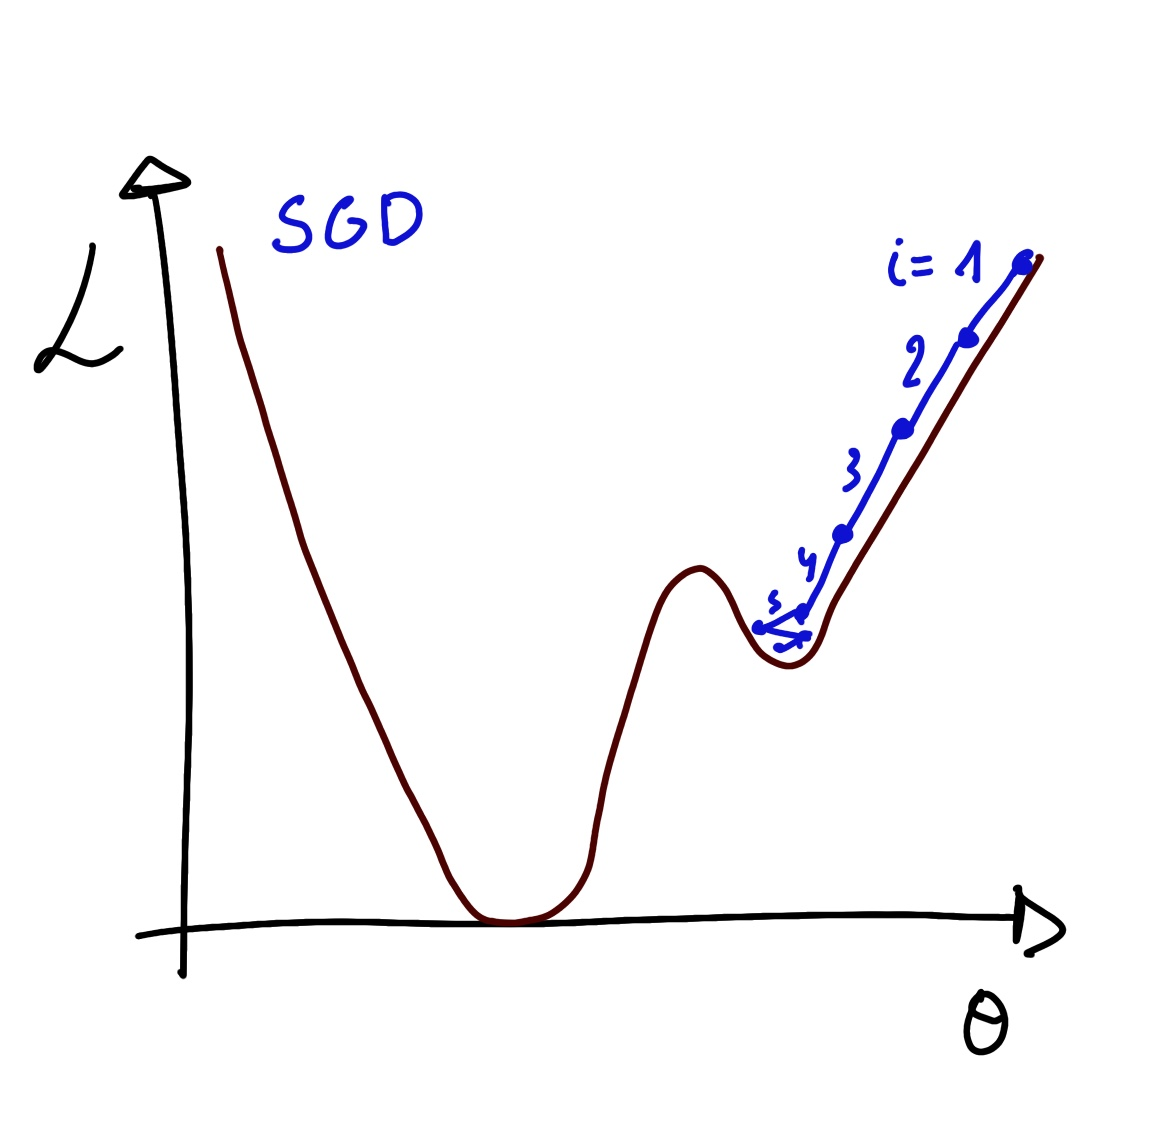
\includegraphics[height=6cm]{images/ml/sgd.jpg}
    \caption{Illustration of SGD falling into a local minima}
    \label{fig:ml:sgd}
  \end{subfigure}
  \hfill
  \begin{subfigure}[t]{0.48\linewidth}
    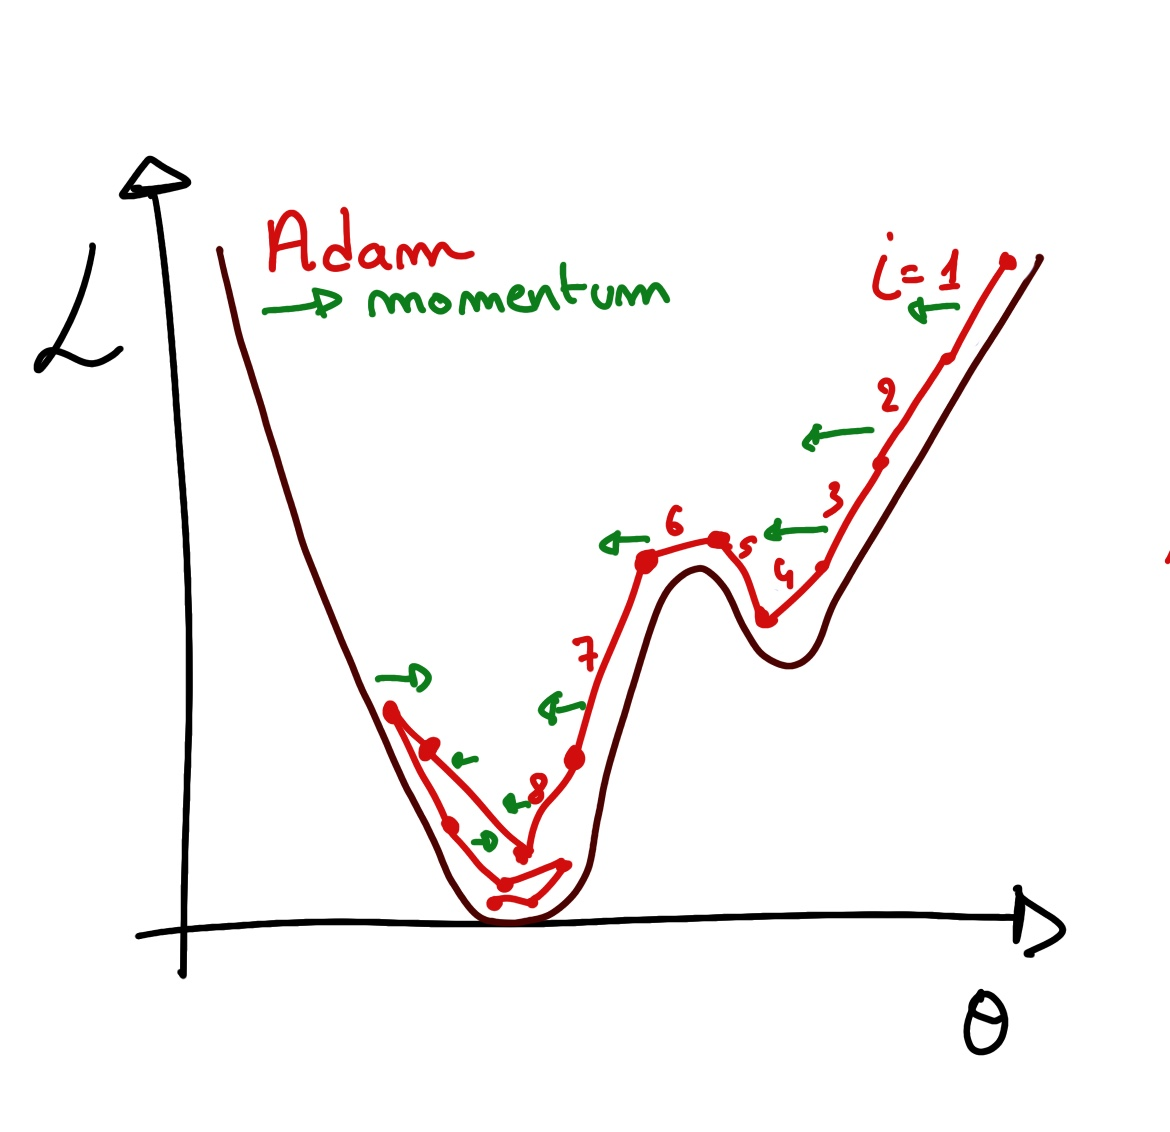
\includegraphics[height=6cm]{images/ml/Adam.jpg}
    \caption{Illustration of the Adam momentum allowing it to overcome local minima}
    \label{fig:ml:adam}
  \end{subfigure}
  \caption{}
\end{figure}

\subsubsection{Learning Rate (LR) Schedules}

The learning rate plays a crucial role in determining how fast or slow the model converges. If the learning rate is too high (Fig. \ref{fig:ml:optims:mae}), the model may skip over the optimal solution, whereas a low learning rate (Fig. \ref{fig:ml:optims:mse}) can slow down the convergence process, leading to inefficient training. To address this, learning rate schedulers are employed.

Using a learning rate scheduler allows the optimizer to take larger steps in the early stages of training, where rapid learning is beneficial, and progressively smaller steps as the model approaches convergence. This strategy is especially useful in JUNO, where early learning from noisy data may require coarse adjustments, but fine-tuning is needed later to accurately capture subtle event characteristics.

\begin{figure}
  \centering
  \begin{subfigure}[t]{0.48\linewidth}
    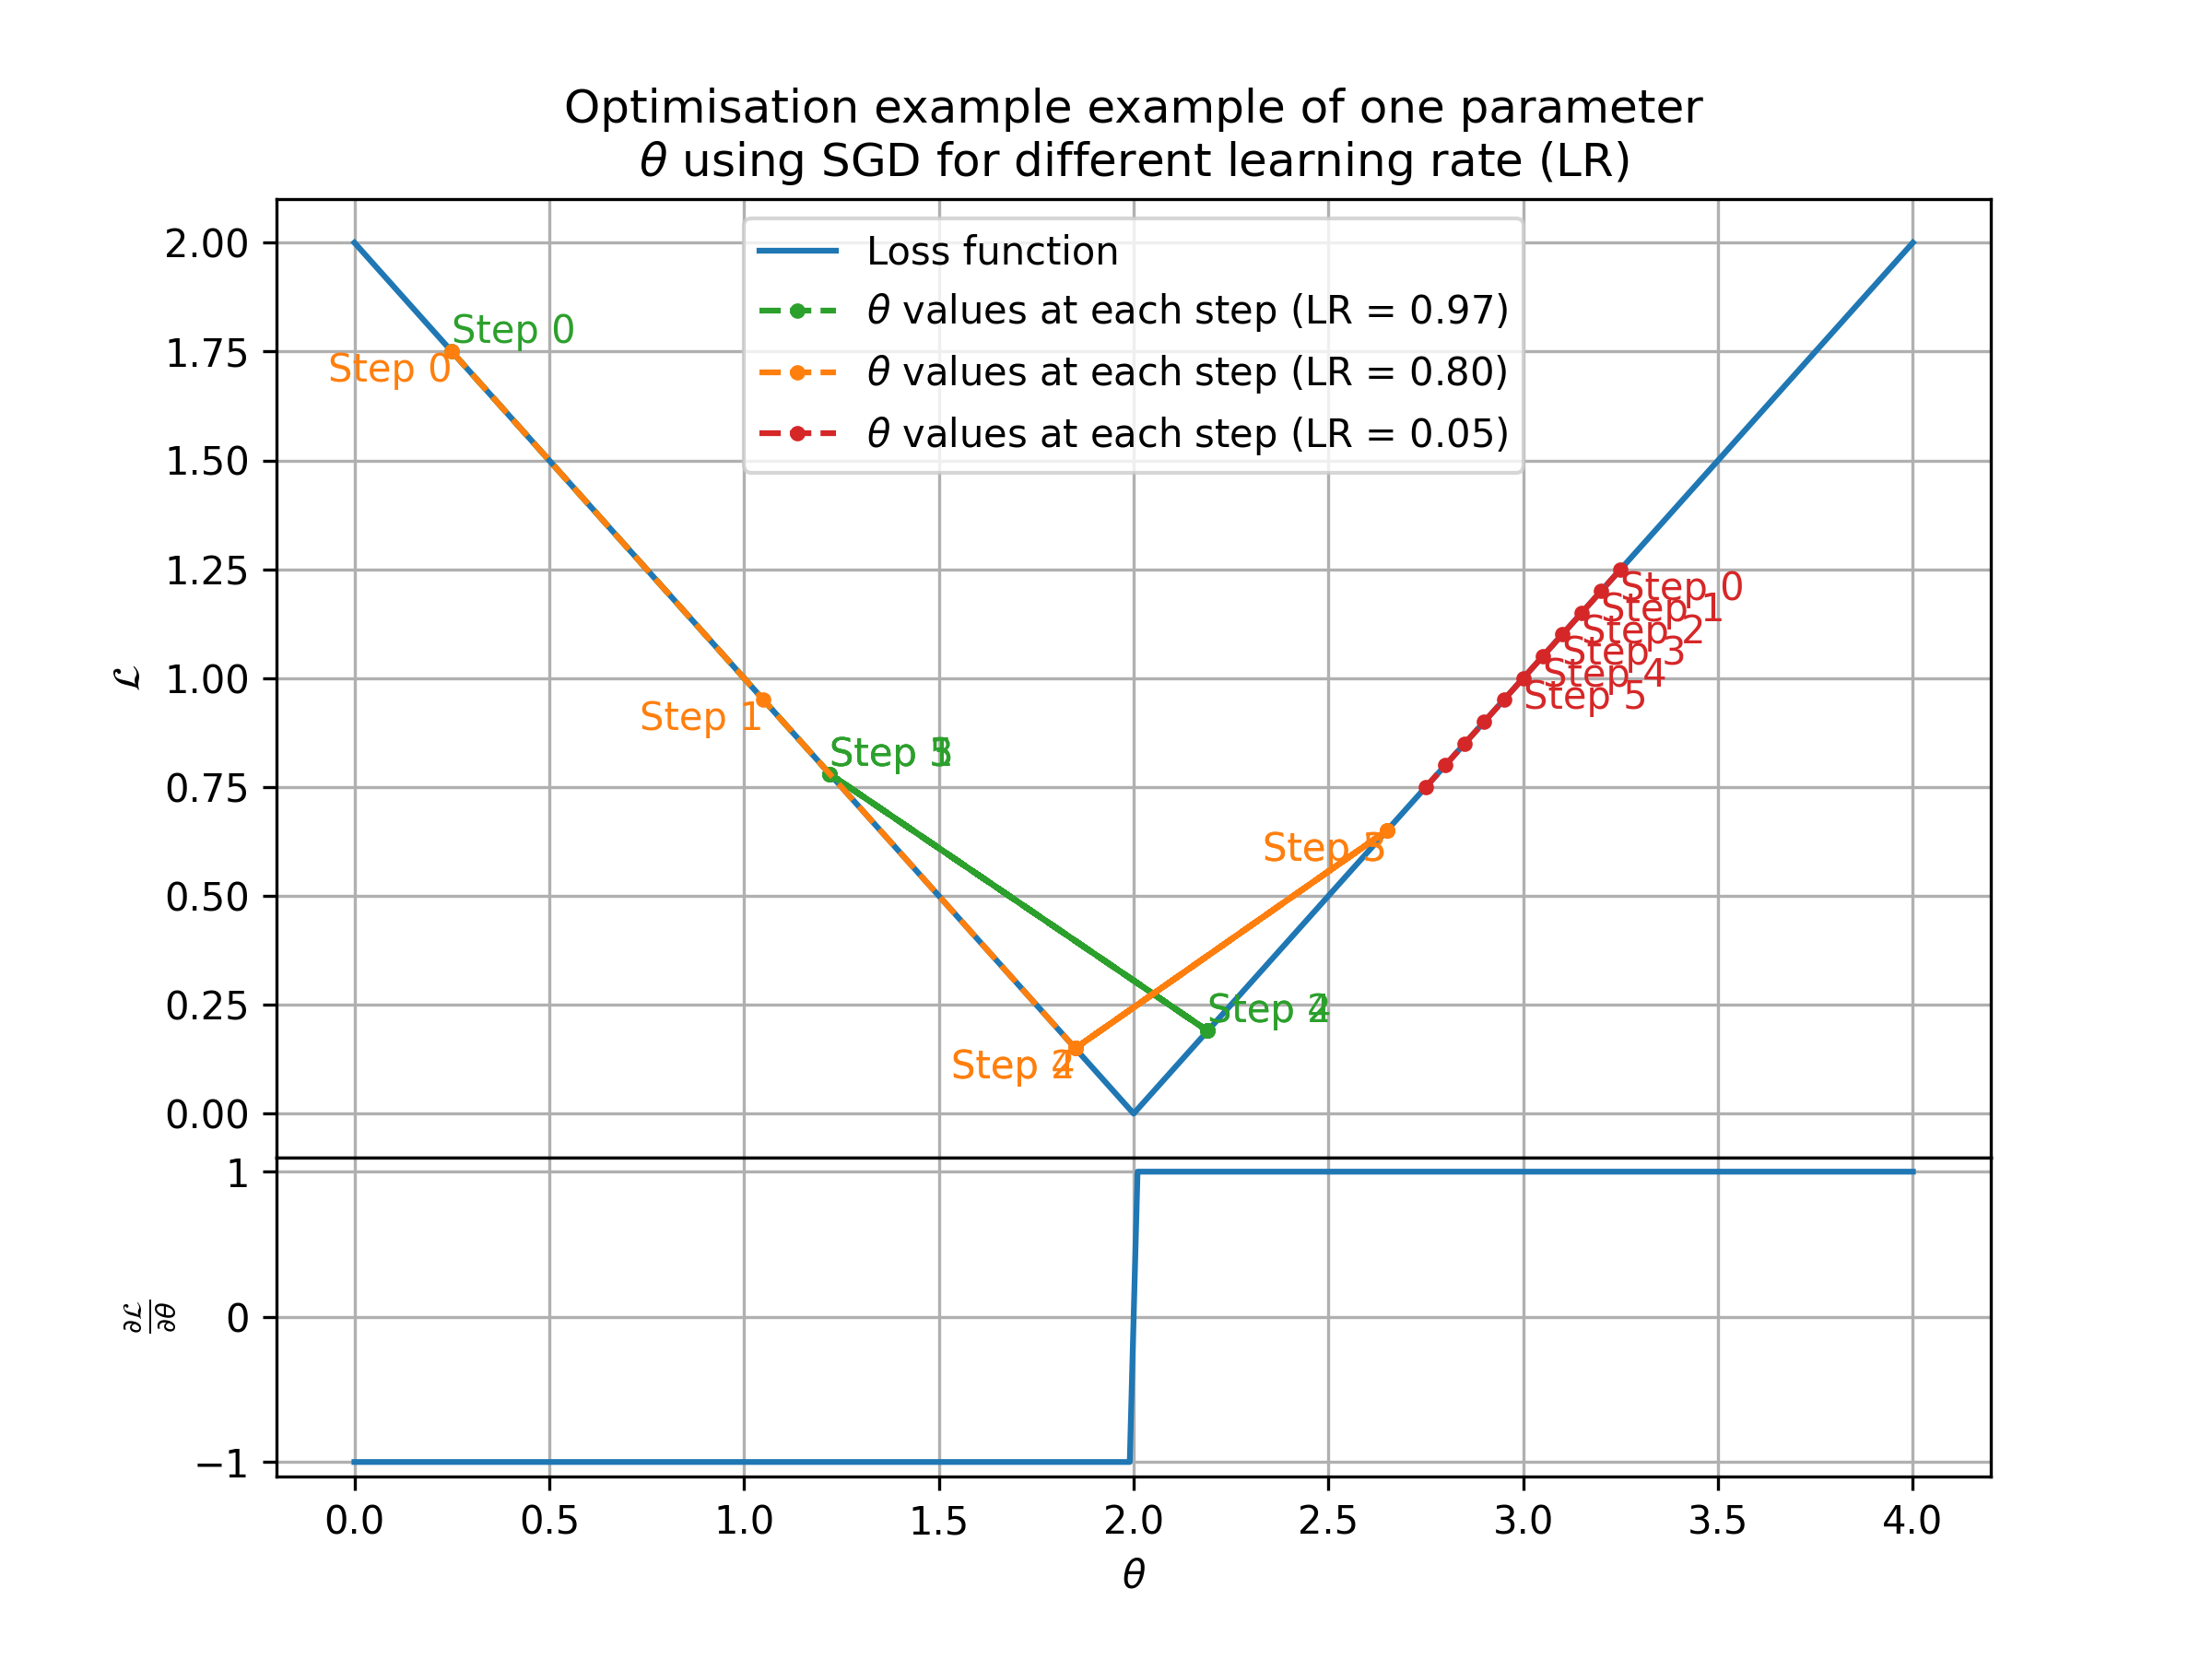
\includegraphics[height=6cm]{scripts/plots/MAE_illustration.png}
    \caption{Illustration of the SGD optimizer on one parameter $\theta$ on the MAE Loss. We see here that it has trouble reaching the minima due to the gradient being constant.}
    \label{fig:ml:optims:mae}
  \end{subfigure}
  \hfill
  \begin{subfigure}[t]{0.48\linewidth}
    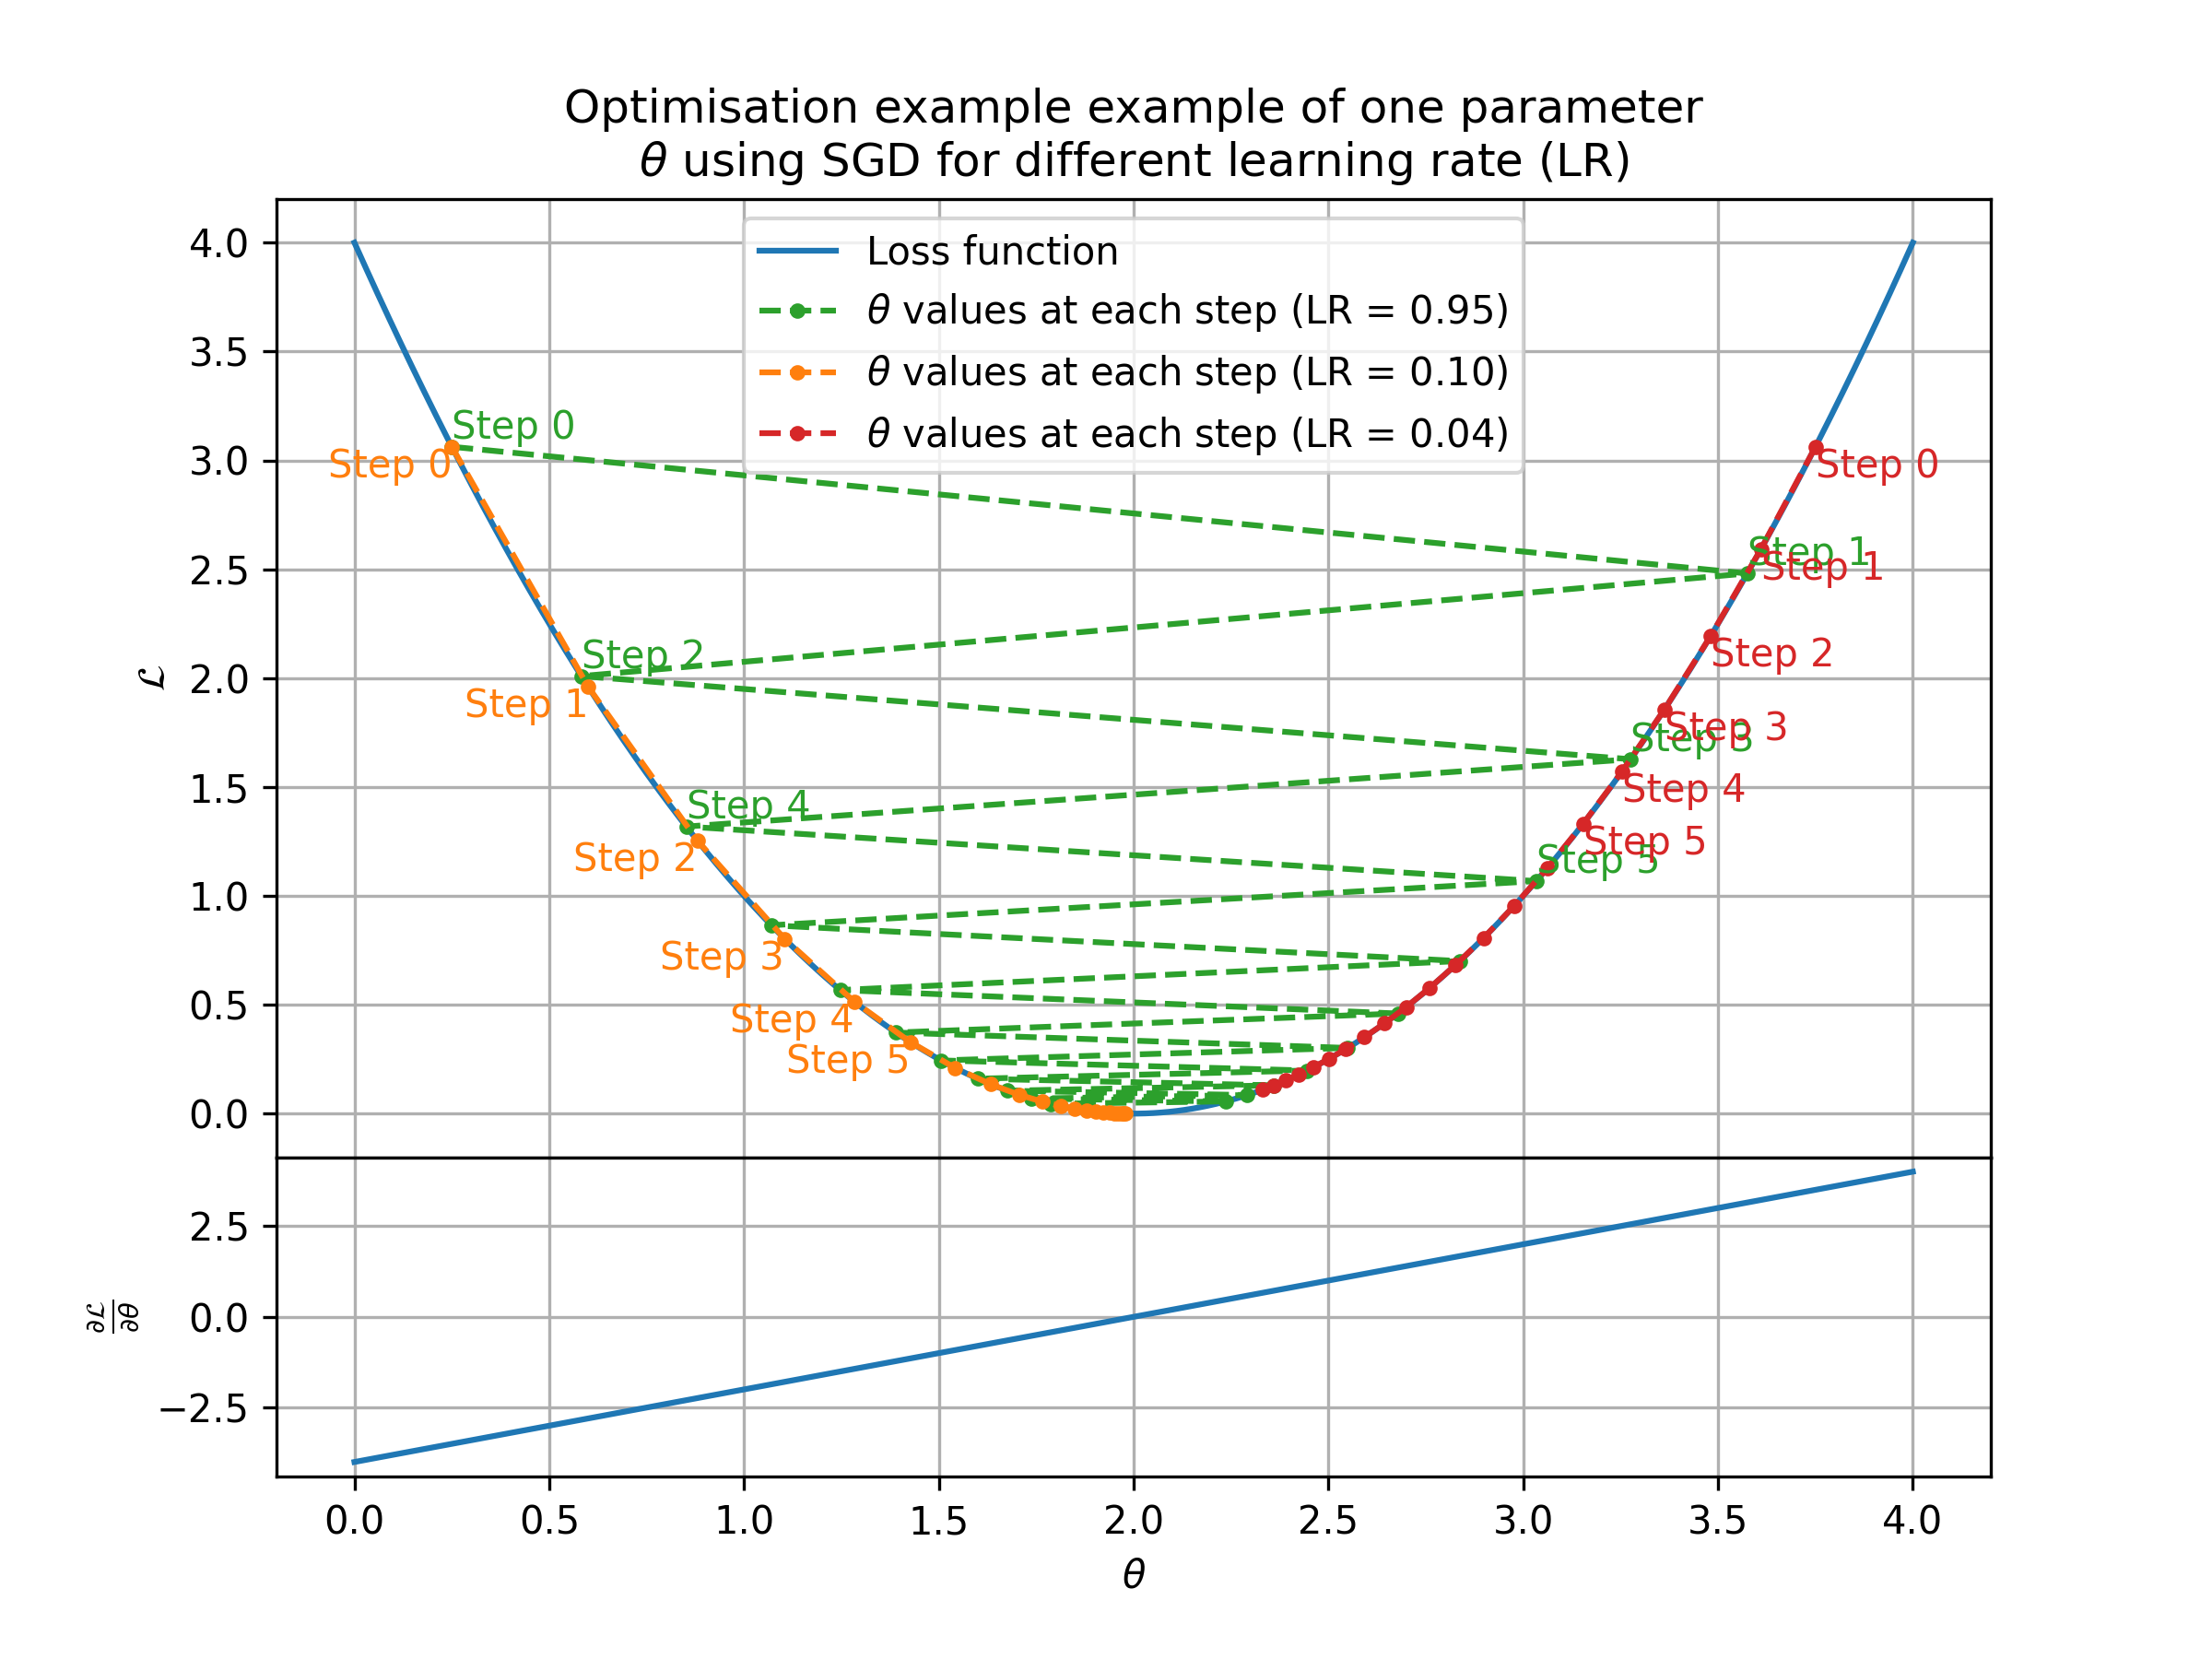
\includegraphics[height=6cm]{scripts/plots/MSE_illustration.png}
    \caption{Illustration of the SGD optimizer on one parameter $\theta$ on the MSE Loss. We see two different behavior: A smooth one (orange and red) when the LR is small enough and a more chaotic one when the LR is too high.}
    \label{fig:ml:optims:mse}
  \end{subfigure}
  \caption{Illustration of the SGD optimizer. In blue is the value of the loss function, orange, green and red are the path taken by the optimized parameter during the training for different LR.}
  \label{fig:ml:optims}
\end{figure}

Another policy that is often use is the save of the best model. In some situation, the loss value after each epoch will strongly oscillate or can even worsen. This policy allow us to keep the best version of the model attained during the training phase.

\subsection{Potential pitfalls}
\label{sec:ml:pitfall}

Apart from being stuck in local minima, there is also other behaviors and effects we want to prevent during training.

\subsubsection{Overtraining}

Overfitting occurs when a neural network memorizes specific details or noise from the training dataset rather than learning a general representation of the underlying data. This is common when the training dataset is small relative to the number of parameters in the network or when the dataset contains specific features that do not generalize well to unseen data. Additionally, training the network for too many epochs can exacerbate this issue. Figure \ref{fig:ml:overtraining} illustrates the impact of overfitting, where the model fits the training data too closely, compromising its ability to generalize.
To detect overfitting, techniques like monitoring the validation loss, early stopping, or employing cross-validation can be employed. In JUNO's context, managing overfitting is critical due to the large volume of data generated by the photomultiplier tubes (PMTs), which may include noise or other artifacts.

Overtraining can be fought in multiple ways, for example:
\begin{itemize}
  \item \textbf{More data}. By having more data in the training dataset, the network will not be able the specificities of every data.
  \item \textbf{Less parameters}. By reducing the number of parameters, we reduce the computing and learning capacities of the network. This will force it to fallback to generalist behaviours.
  \item \textbf{Dropout}. This technique implies to randomly set some neurons to 0, i.e. cutting the relation between two neurons in a layer. By doing this, we force the network to allocate more of its parameter to the features learning, preventing those parameters to be used for overtraining.
  \item \textbf{Early stopping}. During the training we monitor the network performance over a validation dataset. The network does not train on this dataset and thus cannot learn its specificities. If the loss on the training dataset diverge too much from the loss on the validation dataset, we can stop the training earlier to prevent it from overtraining.
\end{itemize}

\begin{figure}
  \centering
  \begin{subfigure}[t]{0.48\linewidth}
    \centering
    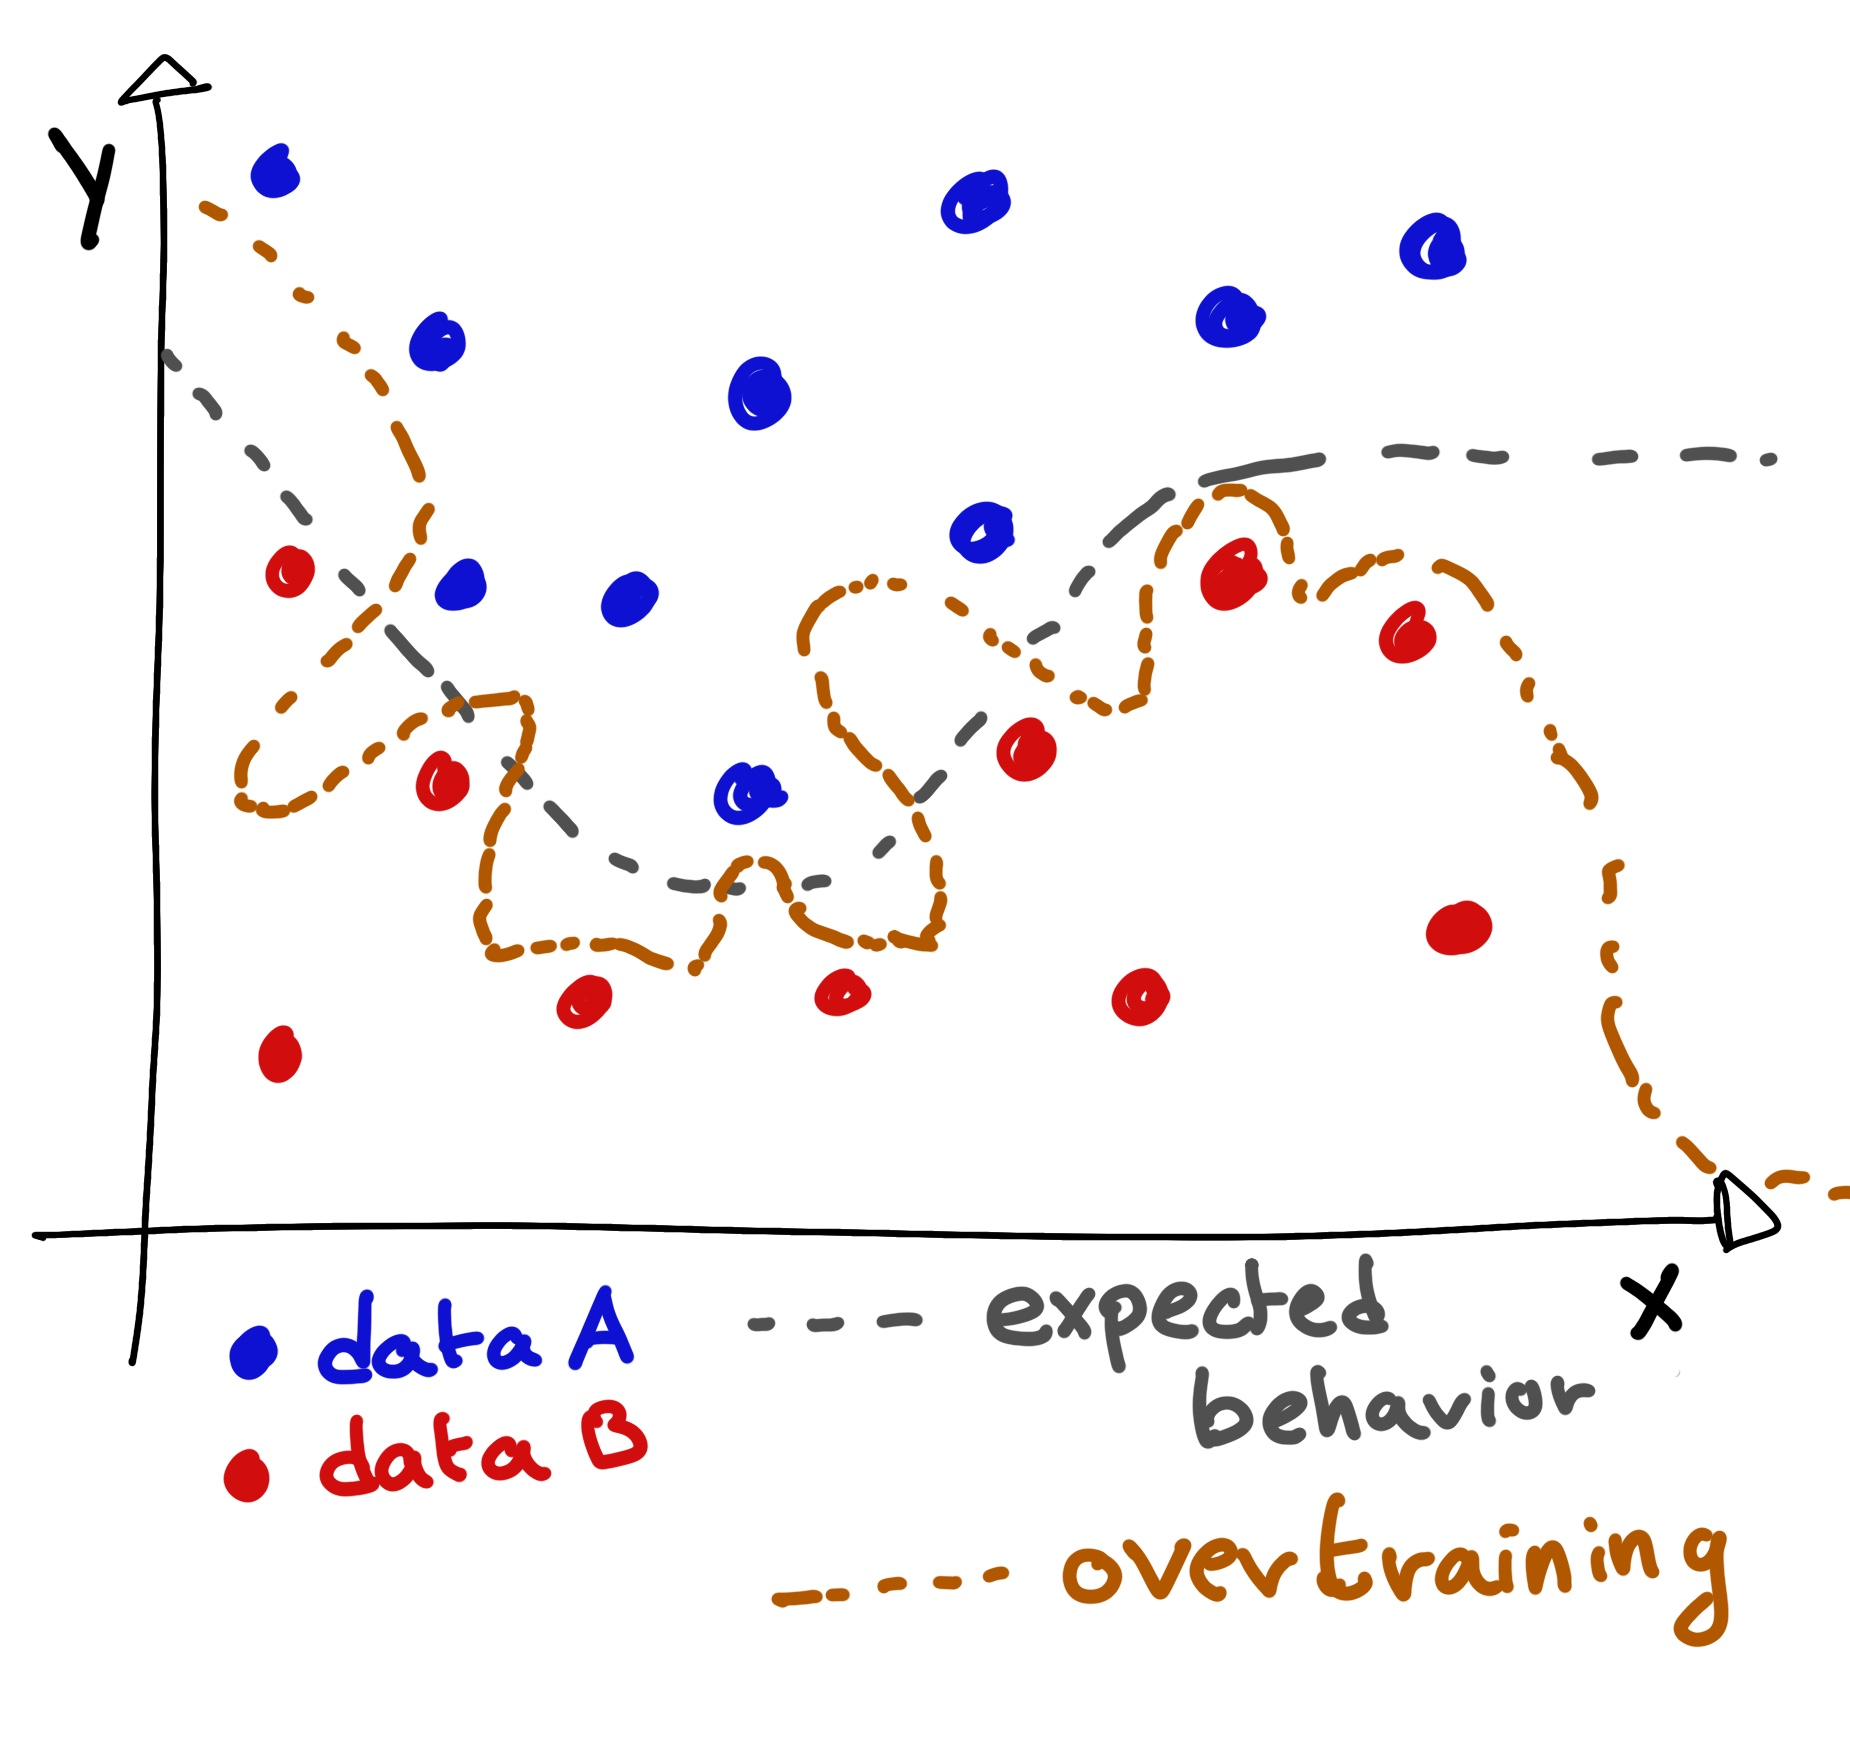
\includegraphics[height=6cm]{images/ml/overtraining.jpg}
    \caption{Illustration of overtraining. The task at hand is to determine depending on two input variable $x$ and $y$ if the data belong to the dataset $A$ or the dataset $B$. The expected boundary between the two dataset is represented in grey. A possible boundary learnt by overtraining is represented in brown.}
    \label{fig:ml:overtraining}
  \end{subfigure}
  \hfill
  \begin{subfigure}[t]{0.48\linewidth}
    \centering
    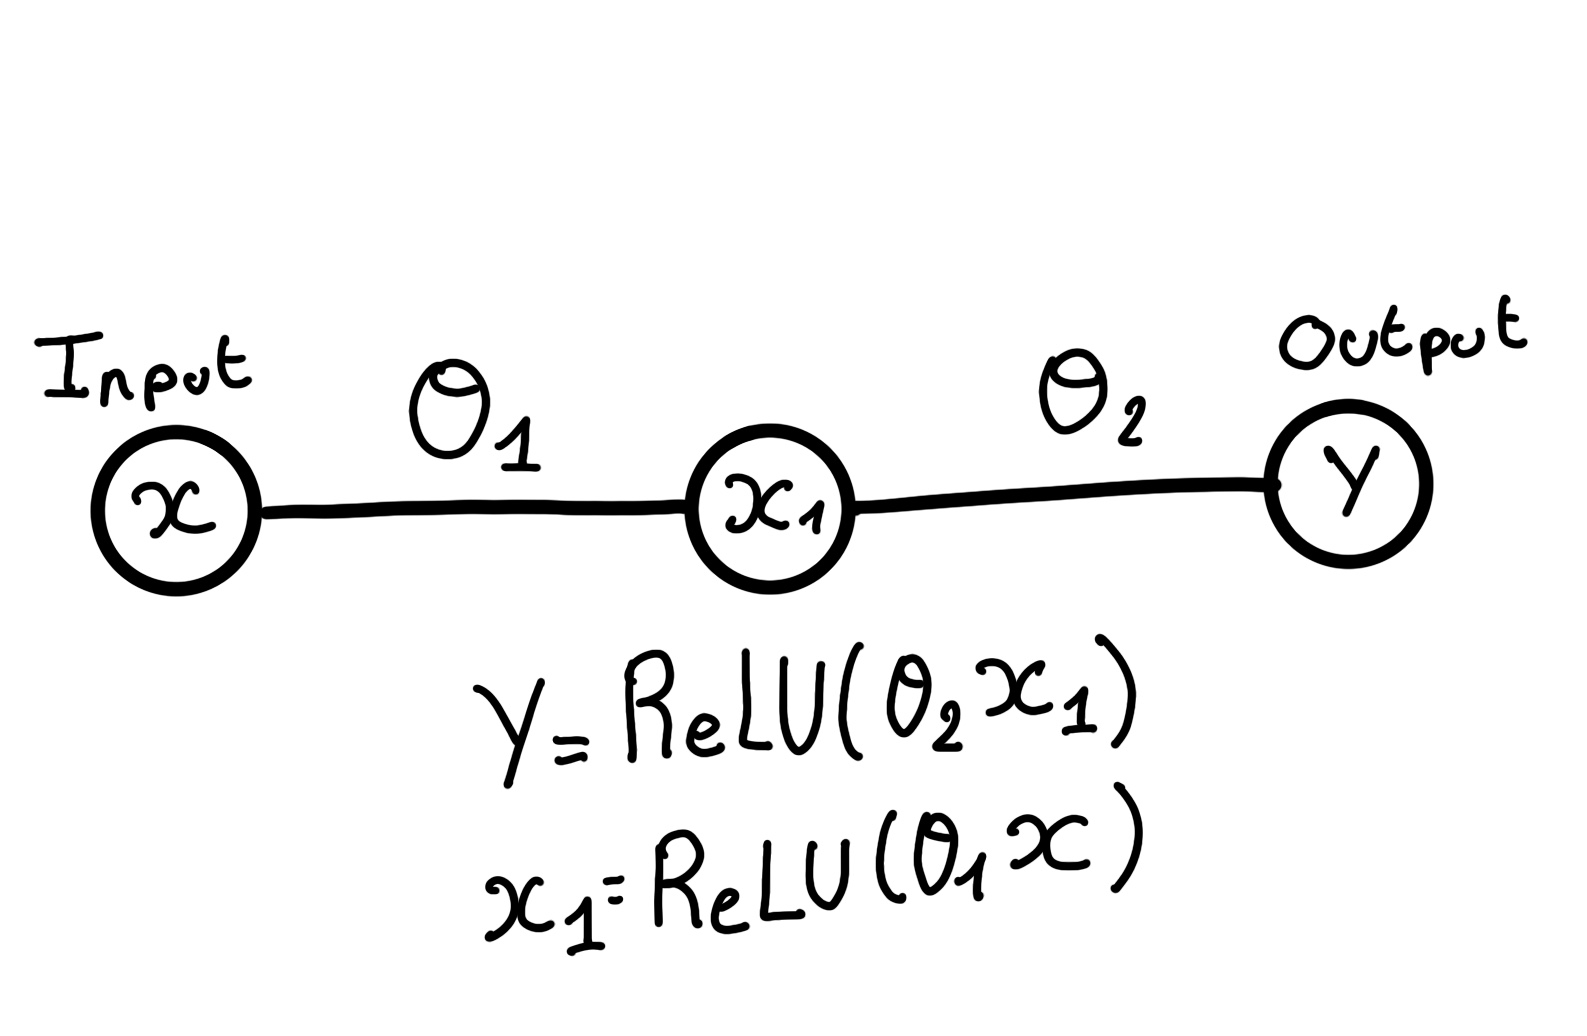
\includegraphics[height=6cm]{images/ml/vanishing_illus.jpg}
    \caption{Illustration of a very simple NN}
    \label{fig:ml:vanishing}
  \end{subfigure}
  \caption{}
\end{figure}

\subsubsection{Gradient vanishing}
Gradient vanishing is the effect of the gradient being so small for the early layers that the parameters are barely updated after each step. This cause the network to be unable to converge to the minima.

This comes from the way the gradient descent is calculated. Imagine a simple network composed of three fully connected layers: the input layer, a intermediate layer and the output layer. Let $L$ be the loss, $\theta_1$ the parameter between the input and the intermediate layer and $\theta_2$ the parameter between the intermediate and output layer. This network is schematized in Figure \ref{fig:ml:vanishing}.

The gradient for $\theta_1$ will be computed using the chain rule presented in equation \ref{eq:ml:backward}. Because $\theta_1$ depends on $\theta_2$, if the gradient of $\theta_2$ is small, so will be the gradient of $\theta_1$. Now if we would have much more layer, we can see how the subsequent multiplication of small gradients would lead to very small update of the parameters thus ``\textit{vanishing gradient}''.

Multiple actions can be taken to prevent this effect such as:
\begin{itemize}
  \item \textbf{Batch normalization}: In this case we apply a normalization layer that will normalize the data. It means that we transform the input variable $X$ into a variable $D$ which distribution follow $\langle D \rangle = 0$ and $\sigma D = 1$. This helps the parameters of the network to maintain an appropriate scale.
  \item \textbf{Residual Network (ResNet)} \cite{he_deep_2016}: Residual network is a technique for neural network in which, instead of just sequentially feeding the results of each layer to the next one, you compute a residual over the input data. This technique is illustrated in Figure \ref{fig:ml:resnet}. The reference \cite{he_deep_2016} show empirical evidence of its relevance.
\end{itemize}


\begin{figure}[ht]
  \centering
  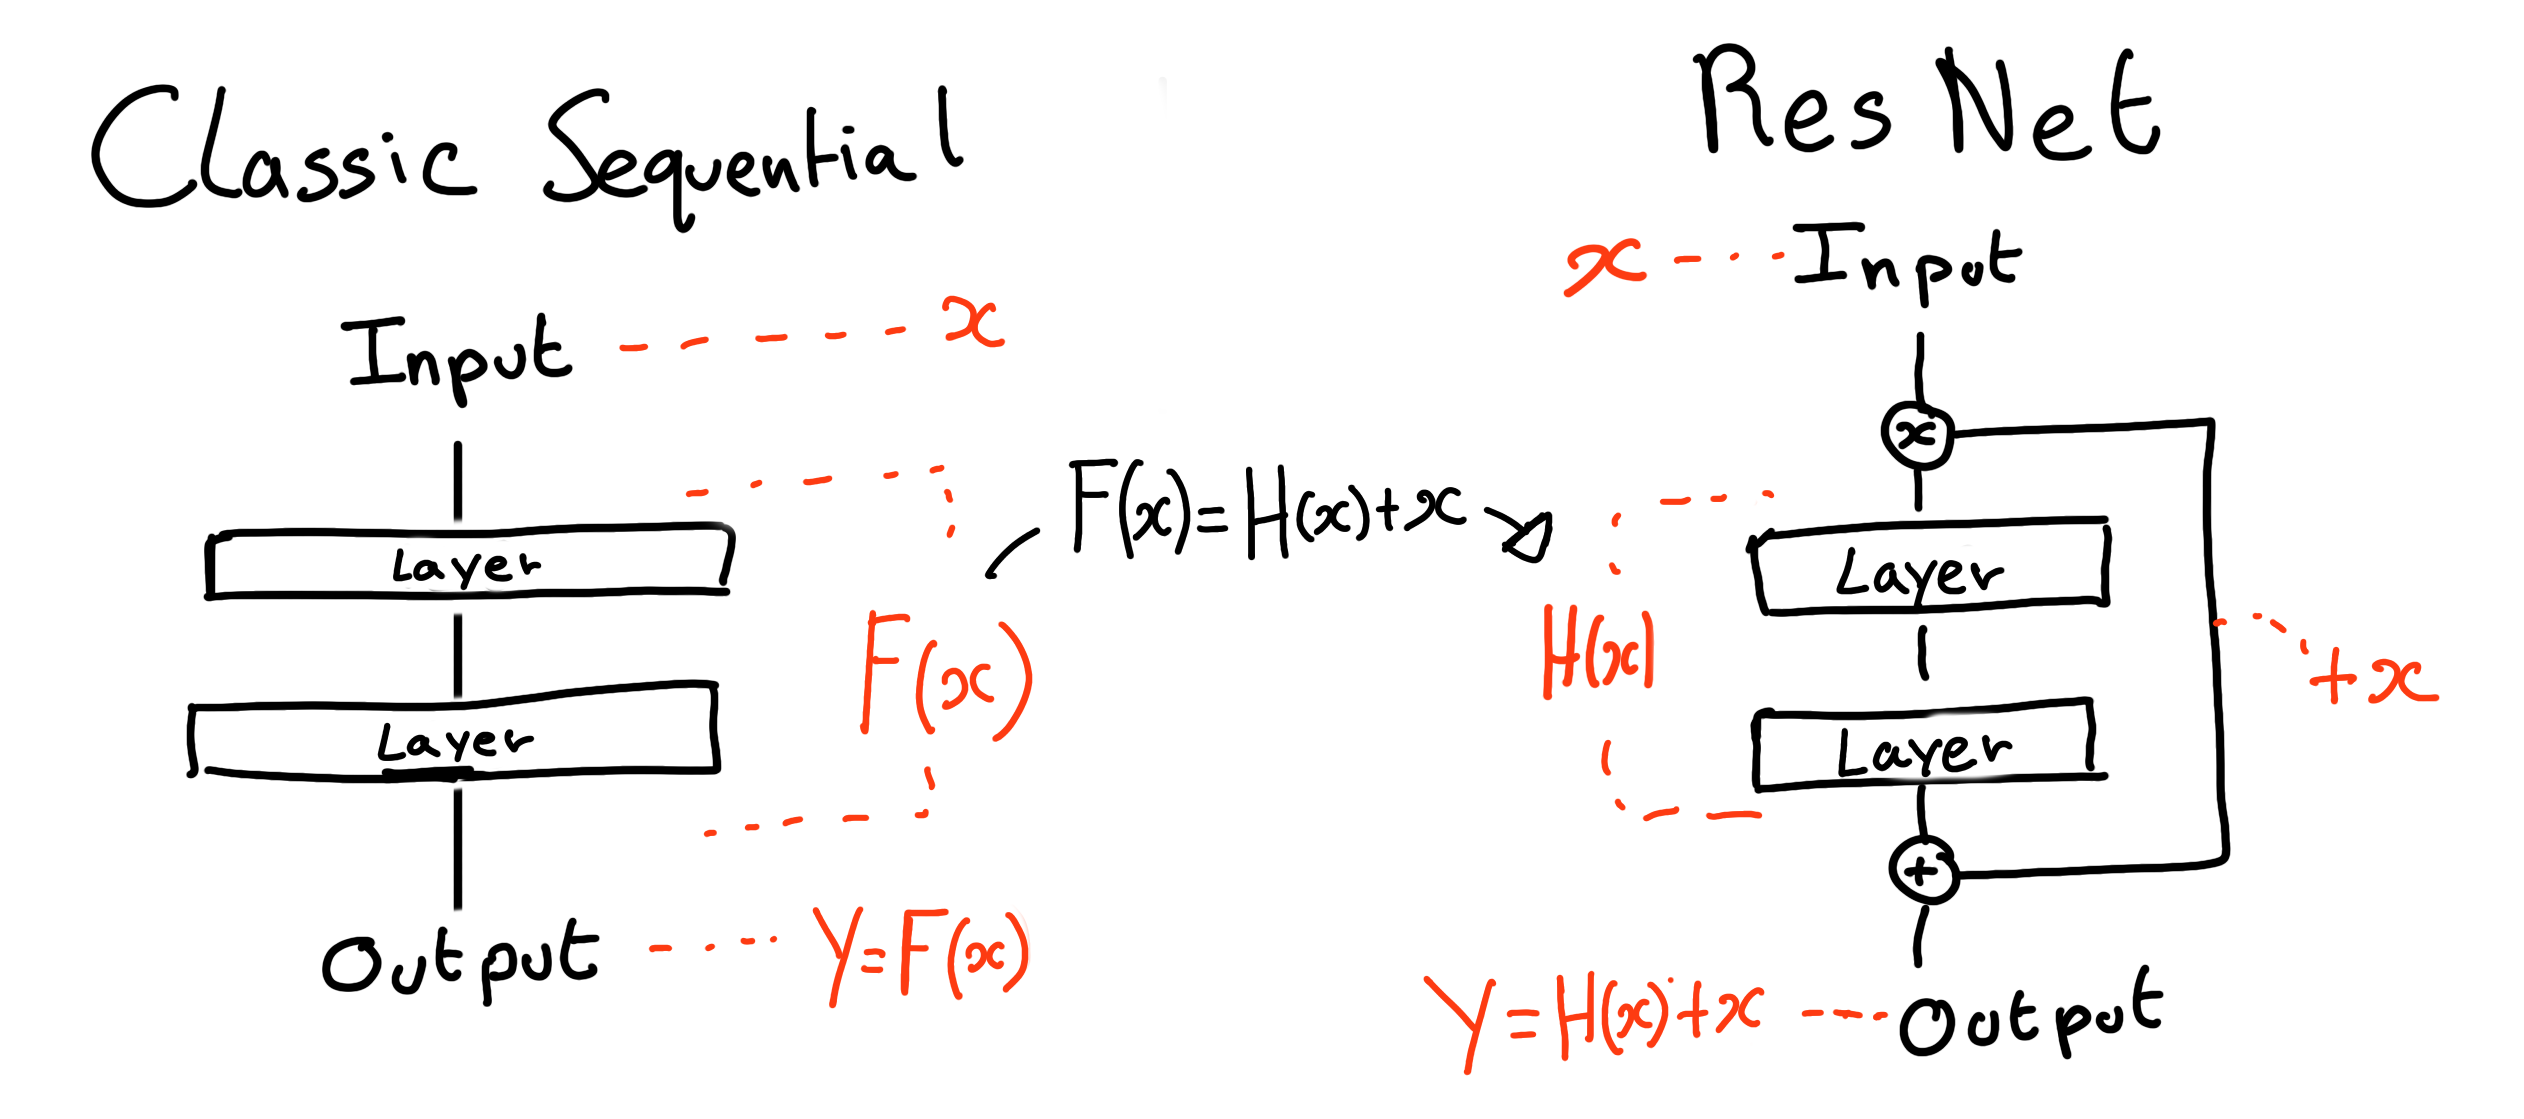
\includegraphics[height=6cm]{images/ml/resnet.png}
  \caption{Illustration of the ResNet framework}
  \label{fig:ml:resnet}
\end{figure}

\subsubsection{Gradient explosion}
Gradient explosion occurs when gradients grow exponentially during backpropagation, causing parameter values to increase dramatically. This is particularly problematic in deep networks where the product of large gradients across layers can lead to unstable updates. In practice, gradient explosion is often caused by large learning rates, poor weight initialization, or nonlinearities in the network.
For illustration, consider that the loss dependency in $\theta$ follow
\begin{align*}
  \mathcal{L}(\theta) &= \frac{\theta^2}{2} + e^{4\theta} \\
  \frac{\partial \mathcal{L}}{\partial \theta} &= \theta + 4e^{4\theta}
\end{align*}
The explosion is illustrated in Figure \ref{fig:ml:explosion} where we can see that the loss degrade with each step of optimization. In this illustration it is clear that reducing the learning rate suffice but this behaviour can happens in the middle of the training where the learning rate schedule does not permit reactivity.

There exist solutions to prevent this explosions:
\begin{itemize}
  \item \textbf{Gradient clipping}: Is this case we work on the gradient so that the norm of gradient vector does not exceed a certain threshold. In our illustration in Figure \ref{fig:ml:explosion} the gradient for $\theta > 0$ could be clipped at 3 for example.
  \item \textbf{Batch normalization}: For the same reasons as for gradient vanishing, normalizing the input data help reduce erratic behaviour.
\end{itemize}


\begin{figure}[ht]
  \centering
  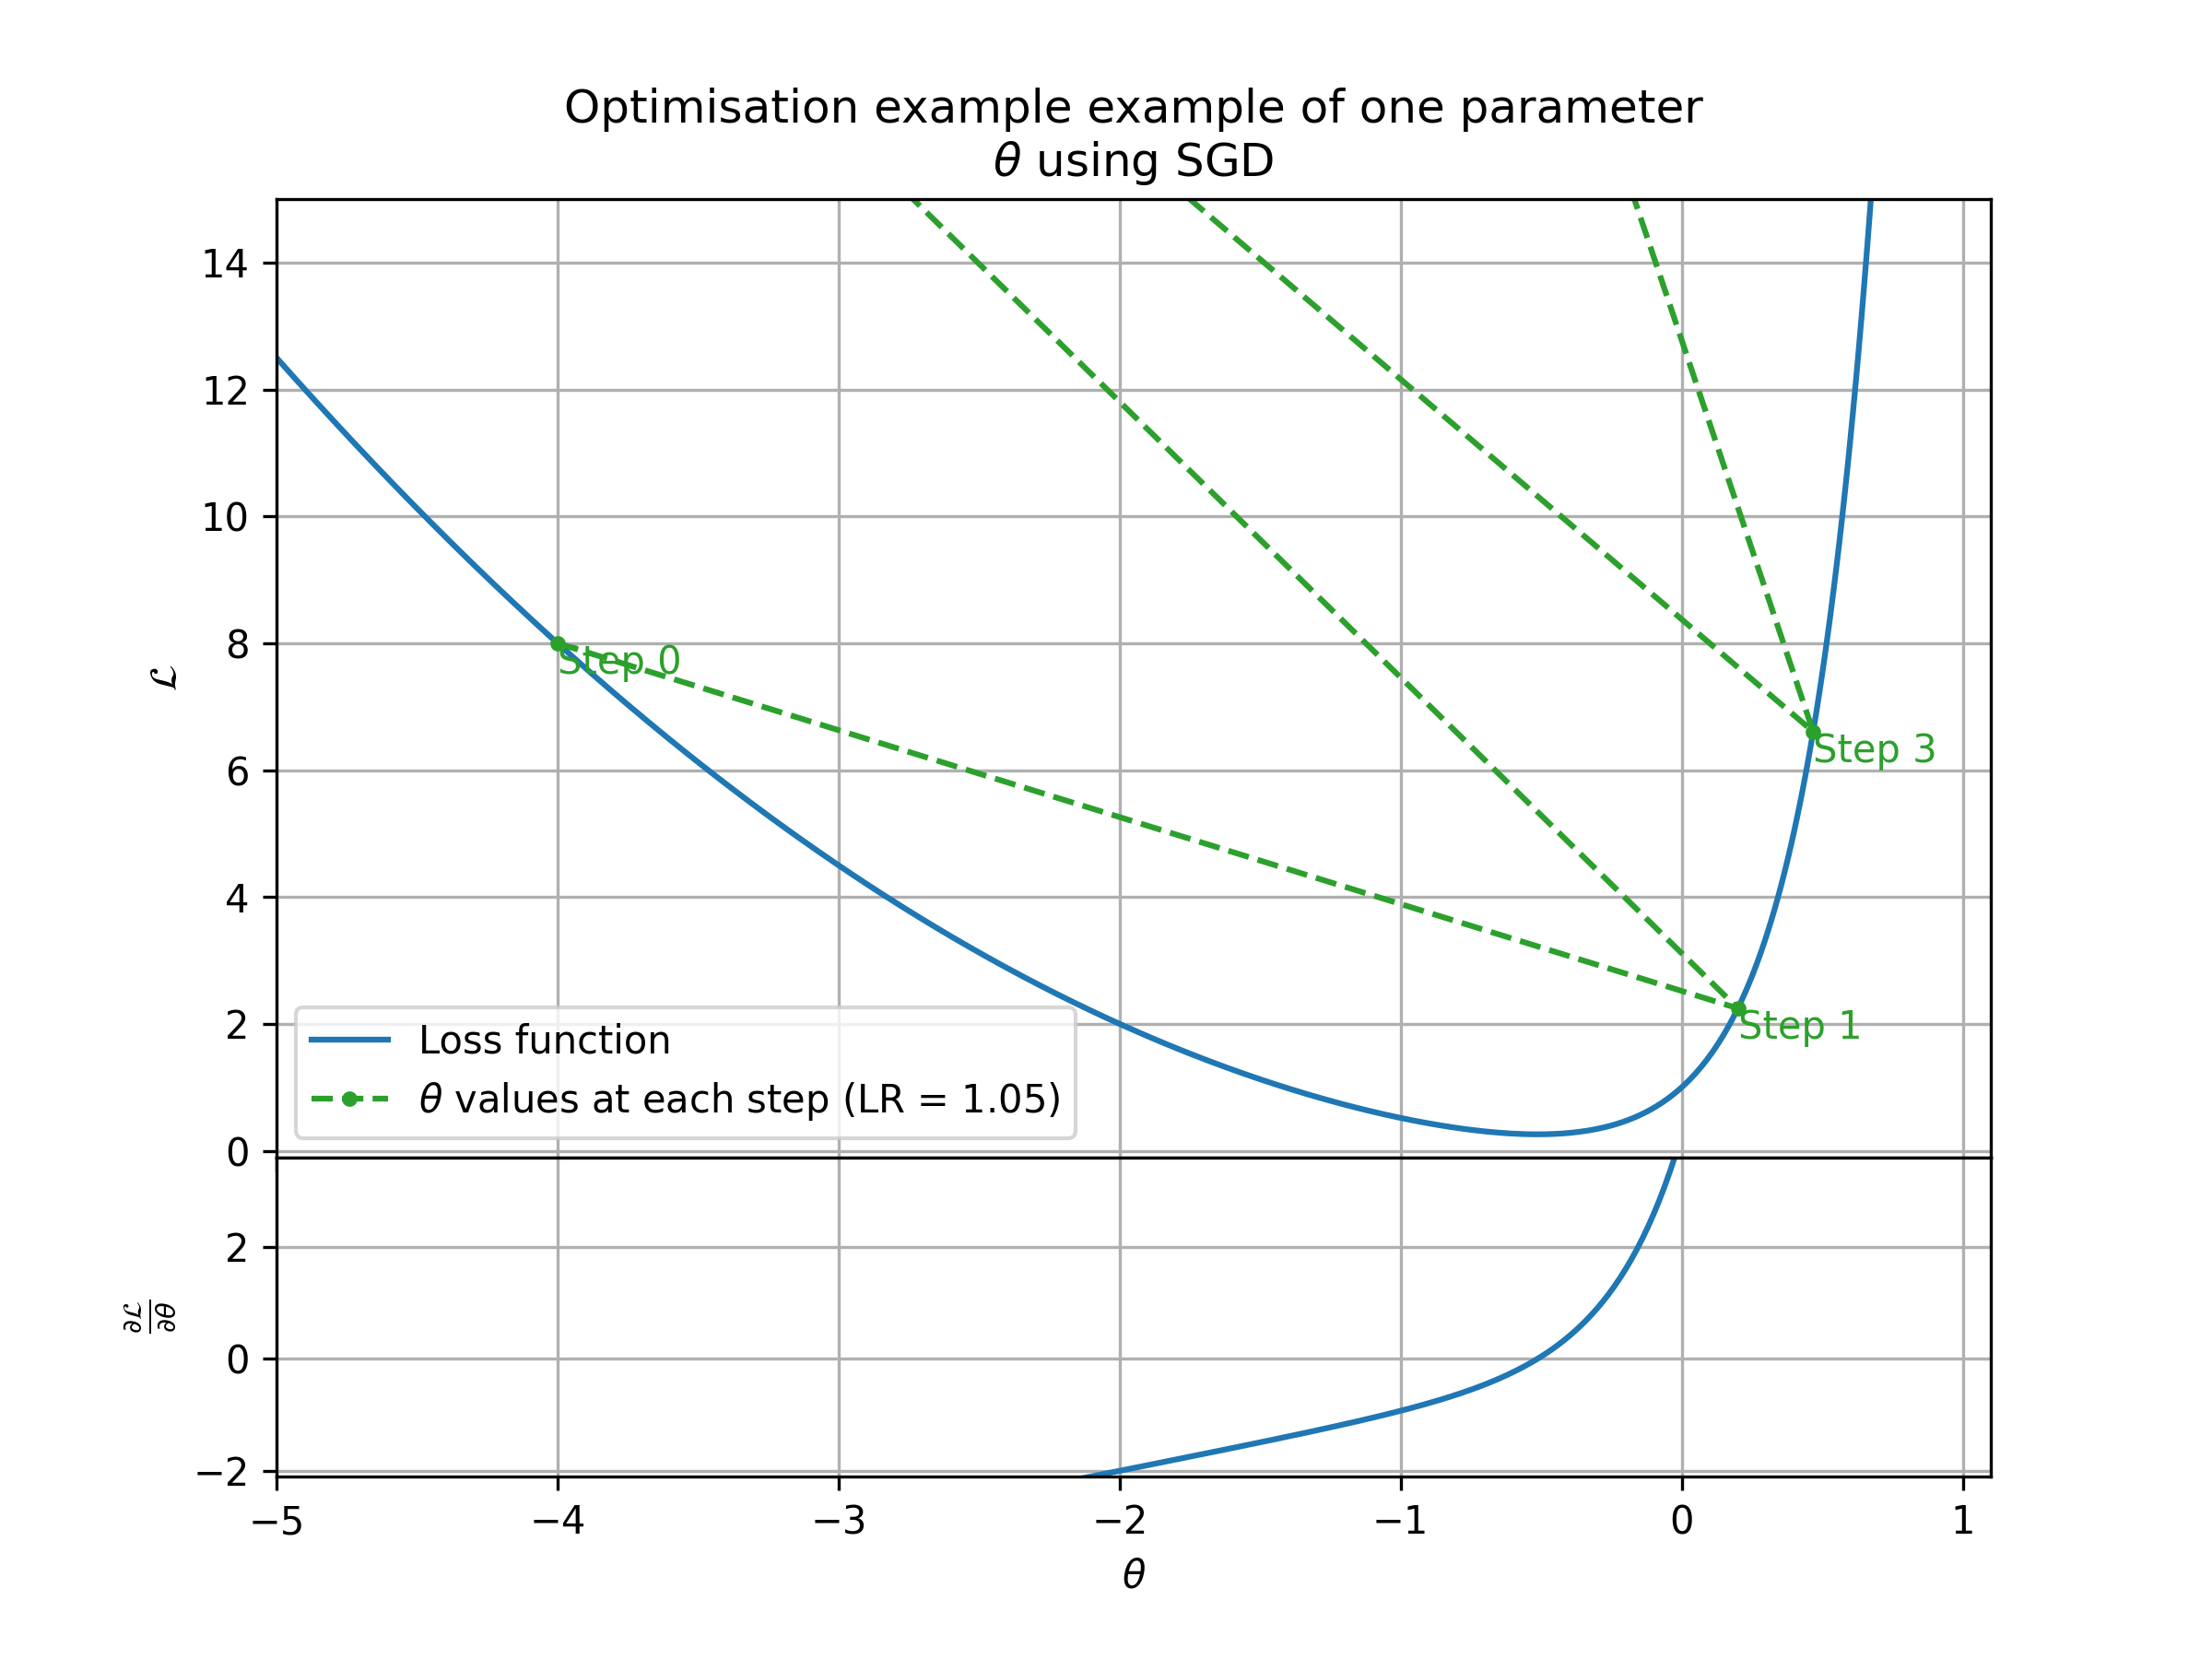
\includegraphics[height=6cm]{scripts/plots/MSE_explosion_illustration.png}
  \caption{Illustration of the gradient explosion. Here it can be solved with a lower learning rate but its not always the case.}
  \label{fig:ml:explosion}
\end{figure}


\section{Neural networks architectures}
\label{sec:ml:architecture}

\subsection{Fully Connected Deep Neural Network (FCDNN)}
\label{sec:ml:fcdnn}

In this thesis, FCDNN serves as a baseline architecture for comparison with more specialized models like CNNs (see Section \ref{sec:ml:cnn}) and GNNs (see section \ref{sec:ml:gnn}), which are better suited to structured or graph-based data. However, FCDNNs are still useful when modeling highly abstract relationships, such as aggregating features from the JUNO PMTs. While they are powerful, their main drawback lies in their inefficiency when dealing with high-dimensional or spatially structured data, which will be addressed with convolutional architectures.
This architecture is the stack of multiple fully connected layers as presented in the Figure \ref{fig:ml:fcdnn}. Most of the time, the classic ReLU function
\begin{equation}
  \label{eq:ml:relu}
  \mathrm{ReLU}(x) = \begin{cases}
    x & \mathrm{if} ~ x \geq 0 \\
    0 & \mathrm{otherwise}
  \end{cases}
\end{equation}
is used as activation function. Prelu and Sigmoid are also popular choices:


\begin{minipage}{0.5\linewidth}
  \begin{equation}
    \label{sec:ml:sigmoid}
    \mathrm{Sigmoid}(x) = \frac{1}{1+ e^{-x}}
  \end{equation}
\end{minipage}
\begin{minipage}{0.5\linewidth}
  \begin{equation}
    \label{sec:ml:prelu}
    \mathrm{PReLU}(x) = \begin{cases}
      x & \mathrm{if} ~ x \geq 0 \\
      \alpha x & \mathrm{otherwise}
    \end{cases}
  \end{equation}
\end{minipage}


The reasoning behind ReLU and PReLU is that with enough of them, you can mimic any continuous function as illustrated in Figure \ref{fig:ml:relu-mimic}. Sigmoid is more used in case of classification, its behavior going hand in hand with the Cross Entropy loss function used in classification problems.

\begin{figure}[ht]
  \begin{subfigure}[t]{0.48\textwidth}
    \centering
    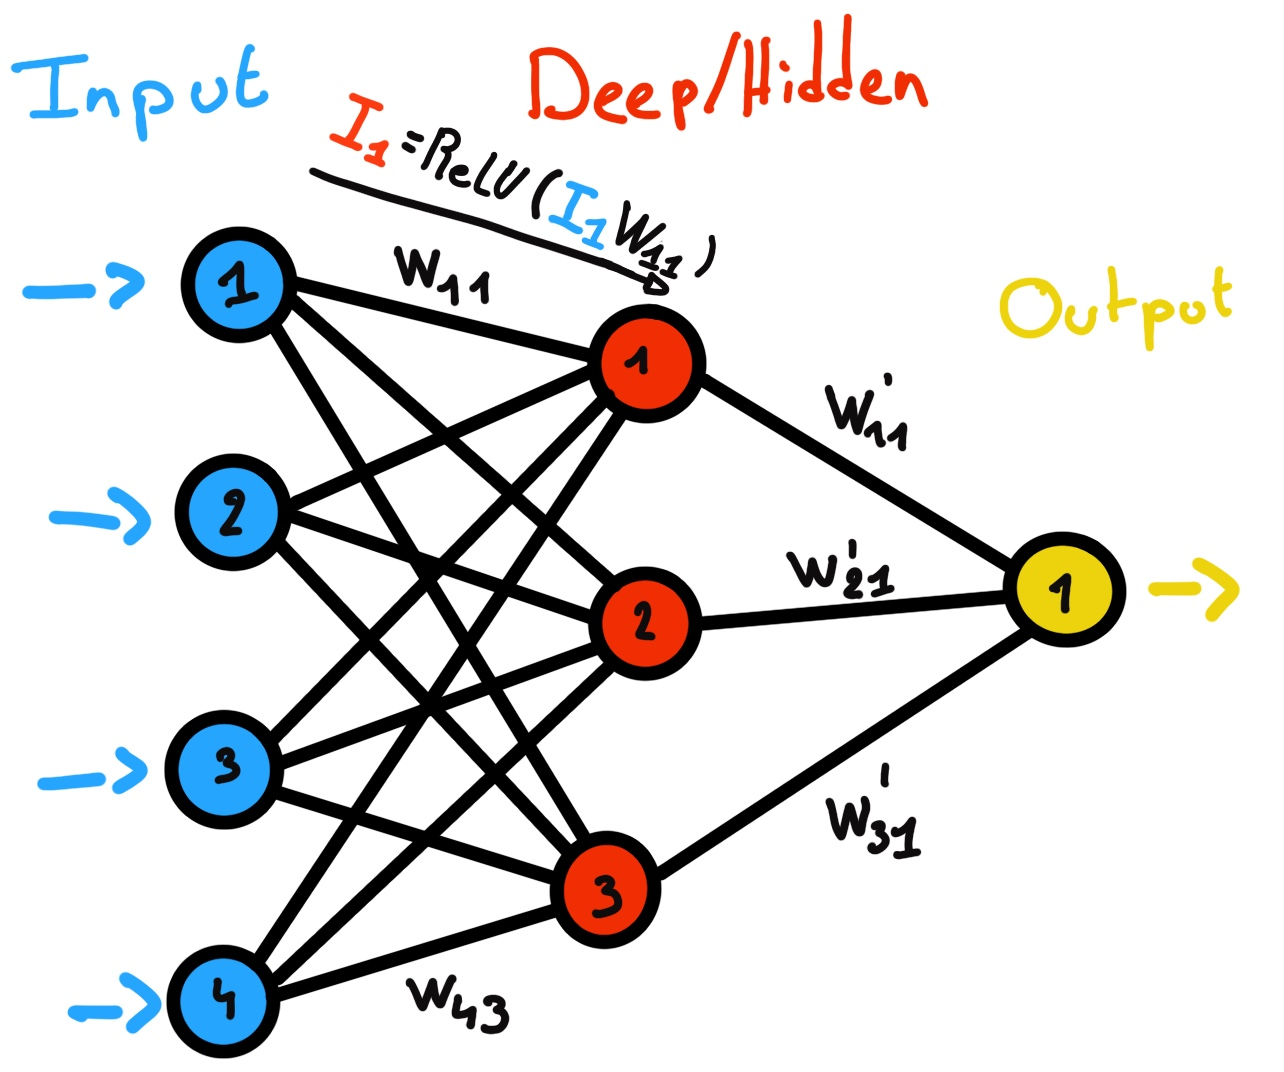
\includegraphics[height=6cm]{images/ml/fcdnn_scheme.jpg}
    \caption{Schema of a FCDNN}
    \label{fig:ml:fcdnn}
  \end{subfigure}
  \hfill
  \begin{subfigure}[t]{0.48\textwidth}
    \centering
    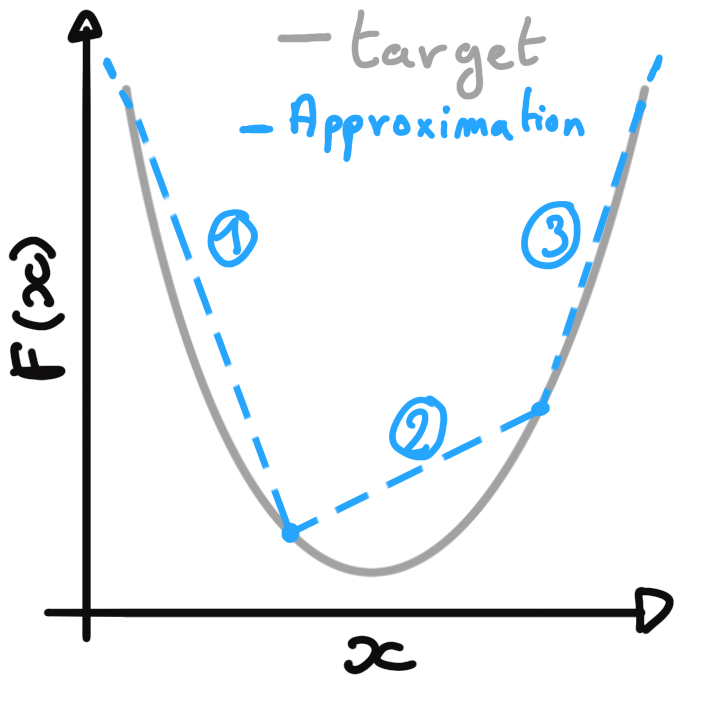
\includegraphics[height=6cm]{images/ml/relu_approx.png}
    \caption{Illustration of a composition of ReLU ``approximating'' a function. (1) No ReLU is taking effect (2) One ReLU is activating (3) Another ReLU is activating}
    \label{fig:ml:relu-mimic}
  \end{subfigure}
  \caption{}
\end{figure}

Due to its simplicity, FCDNN are also used as basic pieces for more complex architectures such as the CNN and GNN that will be presented in the next sections.

\subsection{Convolutional Neural Network (CNN)}
\label{sec:ml:cnn}

It's not trivial to describe in text the principles of Convolutional Neural Network (CNN) and how they works. We try a general description below followed by a step by step description of a concrete example.

Convolutional Neural Networks are a family of neural networks that use discrete convolution filters, as illustrated in an example in Figure \ref{fig:ml:conv_filter}, to process the input data, often images. They are commonly used in image recognition \cite{russakovsky_imagenet_2015} for classification or regression problematics. Concretely, you multiply element-wise a portion of the input data, in the case of an image, a small part of the image, with a kernel of same dimension. In Figure \ref{fig:ml:conv_filter}, we multiply the $3\times3$ pixels sub-image with the $3\times3$ kernel.

Their filters scan the input data, highlighting patterns of interest, this scanning procedure making them translation-invariant. In the concrete case of Figure \ref{fig:ml:conv_filter}, for each pixel of the input image, we group it with the 8 neighbours pixel and produce a new pixel that correspond to the output image. For the pixel on the edges that do not have neighbours, we either create ``imaginary'' pixel with the value 0 or we just ignore them. If we ignore them, the output image will posses fewer pixels than the input image. We see that the operation do not care where is the pattern of interest in the images, the filter output will be \textit{invariant} whatever \textit{translation} is applied to the image.

This invariance mean that they are capable of detecting oriented features independently of their location on the image.
These filters scan the input, highlighting important features like edges or textures, which in JUNO's case could represent spatial correlations in the timing and charge data across the detector. As the network goes deeper, it can capture more complex and abstract features, making it ideal for detecting nuanced particle interactions.
Again taking \ref{fig:ml:conv_filter} as an example, with only the 9 parameters composing the kernel, we can highlight the contour of the duck by looking at the ``yellowness'' of the pixels.

The learning parameters of CNNs are the kernels components, the network thus learn the optimal filters to extract the desired features.

The convolution layers are commonly chained \cite{simonyan_very_2015}, reducing the input dimension while increasing the number of filters. The idea behind is that the first layers will process local informations and the latest layers will process more global informations, as the latest convolution filters will process the results of the preceding that themself have processed local information. To try to preserve the amount of information, we tend to grow the numbers of filters for each division of the input data.
The results of the convolution filters is commonly then flattened and feed to a smaller FCDNN which will process the filters results to yield the desired output.

\begin{figure}[ht]
  \centering
  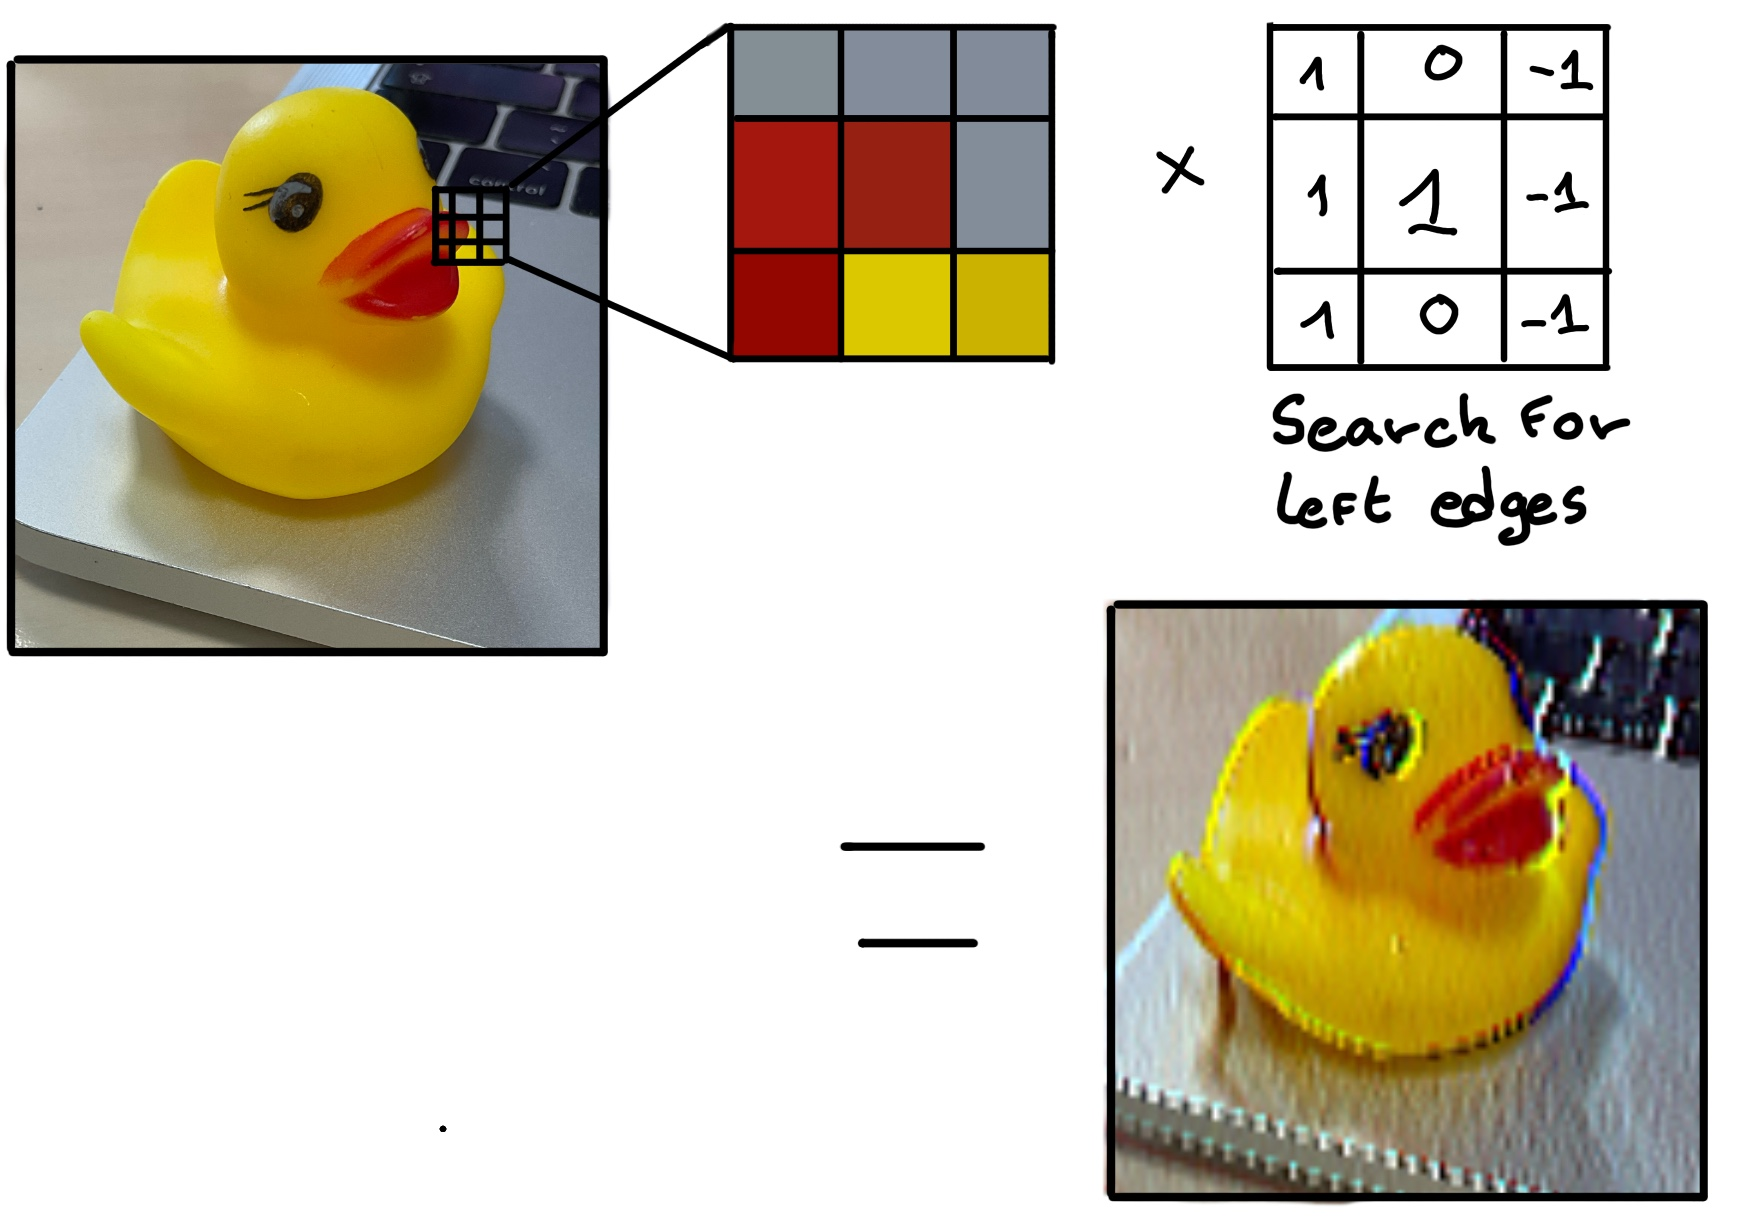
\includegraphics[height=6cm]{images/ml/convolution_exammple.jpg}
  \caption{Illustration of the effect of a convolution filter. Here we apply a filter with the aim do detect left edges. We see in the resulting image that the left edges of the duck are bright yellow where the right edges are dark blue indicating the contour of the object. The convolution was calculated using \cite{allen_generic-github-userimage-convolution-playground_2024}.}
  \label{fig:ml:conv_filter}
\end{figure}

As an example, let's take the Pytorch \cite{ansel_pytorch_2024} example for the MNIST \cite{lecun_gradient-based_1998}, a dataset of black and white images of handwritten digits. Those images are $28 \times 28$ pixels with only one channel corresponding to the grey level of the pixel. Example of images from this dataset are presented in Figure \ref{fig:ml:mnist}

A schema of the CNN used in the Pytorch example is presented in Figure \ref{fig:ml:cnn_mnist}. Using this schema as a reference, the trained network is made of:
\begin{enumerate}
  \item A convolutional layer of $(3 \times 3)$ filters yielding 32 channels. A bias parameter is applied to each channel for a total of $(32 \cdot (3\times3) + 32) = 320$ parameters. The resulting image is $(26\times26 \times 32)$ (26 per 26 pixels with 32 channels). The ReLU activation function is applied to each pixel.
  \item A second convolutional layer of $(3 \times 3)$ filters yielding 64 channels. This channel also posses a bias parameter for a total of $(64 \cdot (3\times3) + 64) = 640$ parameters. Resulting image is $(24\times24\times64)$. This channel also apply a ReLU activation function.
  \item Then comes a $(2\times2)$ max pool layer with a stride of 1 meaning that for each channel the max value of pixels in a $(2\times2)$ block is condensed in a single resulting pixel. The resulting image is $(12 \times 12 \times 64)$.
  \item This image goes through a dropout layer which will set the pixel to 0 with a probability of 0.25. This help prevent overtraining the neural network (see Section \ref{sec:ml:pitfall} for more details).
  \item The data is the flattened i.e. condensed into a vector of $(12 \times 12 \times 64) = 9216$ values.
  \item Then comes a fully connected linear layer (Eq. \ref{eq:ml:fully-connected}) with a ReLU activation that output 128 feature. It needs $(9216 \cdot 128)+ 128 = 1'179'776$ parameters.
  \item This 128 item vector goes through another dropout layer with a probability of $0.5$
  \item The vector is then transformed through a linear layer with ReLU activation. It output 10 values, one for each digit class (0, 1, 2, ..., 9). It need $(128 \cdot 10) + 128 = 1408$ parameters.
  \item Finally the 10 values are normalized using a log softmax function $\mathrm{LogSoftmax}(x_i) = \log \bigg(\frac{\exp(x_i)}{\sum_j \exp(x_j)}\bigg)$. Each of those values are the probability of the input image to be a certain digit.
\end{enumerate}

\begin{figure}[ht]
  \centering
  \begin{subfigure}[t]{0.48\linewidth}
    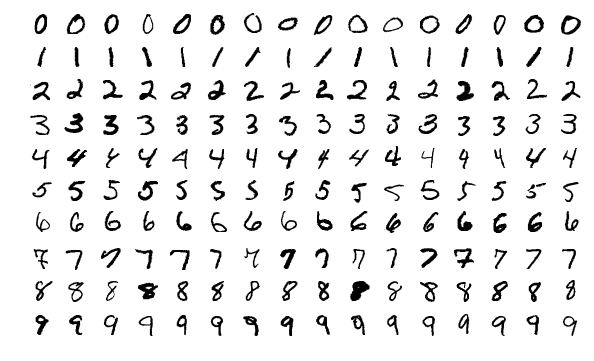
\includegraphics[width=\linewidth]{images/ml/MnistExamples.png}
    \caption{Example of images in the MNIST dataset}
    \label{fig:ml:mnist}
  \end{subfigure}
  \hfill
  \begin{subfigure}[t]{0.48\linewidth}
    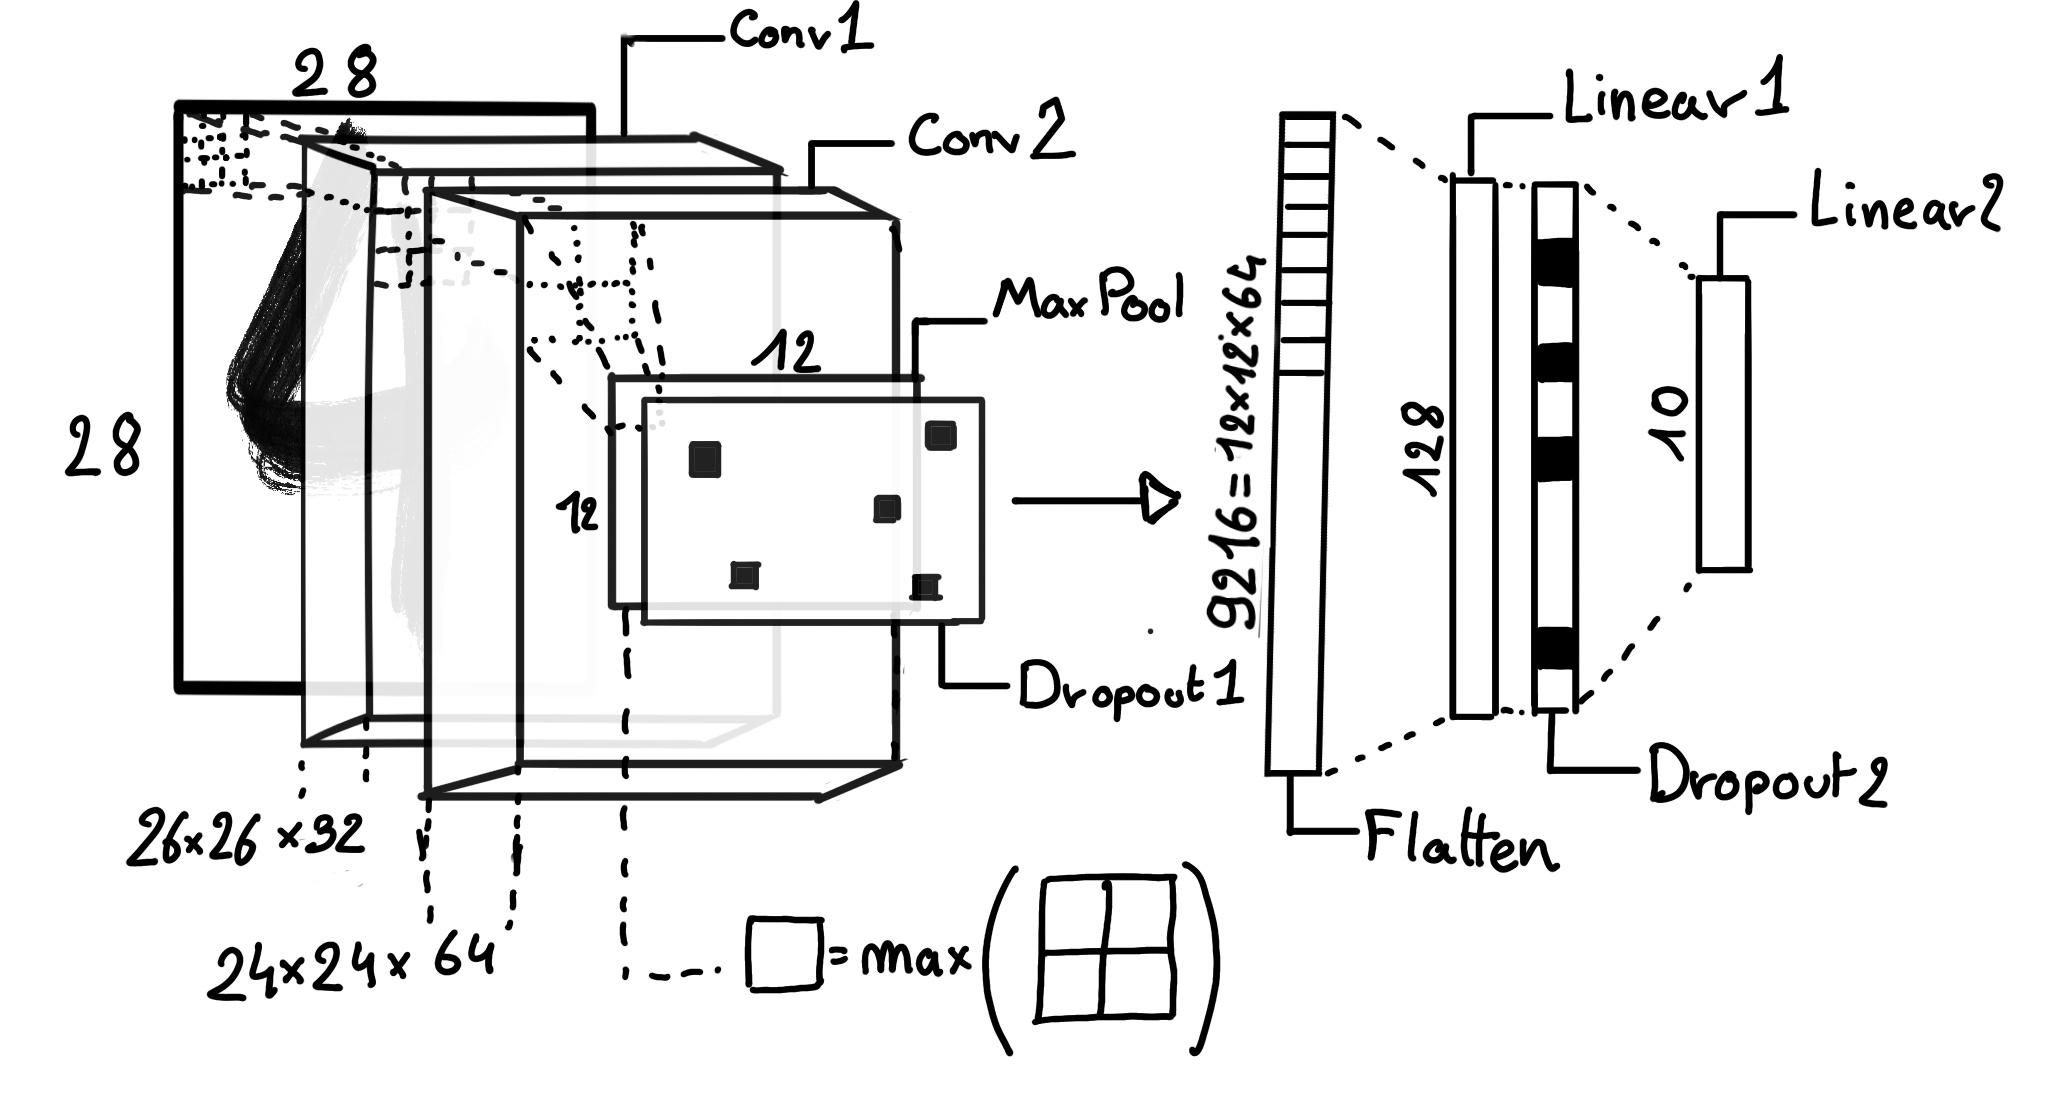
\includegraphics[width=\linewidth]{images/ml/mnist_cnn.jpg}
    \caption{Schema of the CNN used in Pytorch example to process the MNIST dataset}
    \label{fig:ml:cnn_mnist}
  \end{subfigure}
  \caption{}
\end{figure}

The final network needs 1'182'144 parameters or, if we consider each parameters to be a double precision floating point, 9.45 MB of data. To gives a order of magnitude, such neural network is considered ``simple'', train in a matter of minutes on T4 GPU \cite{noauthor_nvidia_nodate} (14 epochs) and reach an accuracy in its prediction of 99\%.


\subsection{Graph Neural Network (GNN)}
\label{sec:ml:gnn}

In GNNs, data is represented as nodes and edges in a graph, which allows us to model the JUNO detector as a network of PMTs, where each PMT is a node and the edges represent relationships such as spatial distance or timing correlations between PMTs. This flexibility enables GNNs to capture complex interactions across the detector geometry that would be difficult to represent with a CNN, as the CNN neighbouring scheme is stucked to the pixels indexing -- the position in the matrix representing the image.

Furthermore, GNNs excel at processing non-Euclidean data, making them a natural fit for the irregular layout of the PMTs in JUNO.
In this thesis, GNNs are applied to model the spatial and temporal relationships between PMTs, enabling more precise event classification and reconstruction. By leveraging the message-passing framework, the GNN can aggregate information from neighboring PMTs, allowing it to detect subtle patterns in the detector's data.

To get deeper in details, we have seen in the previous section, the CNNs are powerful for image processing, and more generally any data that can be expressed as a regular, discrete space and from which the information reside in the dispersion in this space. For an image, the edges of an object and how they assemble. A red square, straight edges with a sharp angle between them, is much less representative of a duck than an yellow sphere, round edges without sharp angles.

This ``image'' projection is not fitted for every problematics. The signals produced by a detector does not always have the properties of images. In the case of JUNO for example, we can create an image of two channels, one for the charge $Q$ and one for the timing $t$ but this image should be spheric. Furthermore JUNO is by nature inhomogeneous, using two different systems : The LPMT and the SPMT. Those two systems have different regime, and thus should be processed differently. We could imagine images with four channels, two for the LPMT and two for the SPMT, or even a branched CNN with one convolution branch for the LPMT and another one for the SPMT. Anyway, the CNN will need to combine the two systems.

To get around the restrictions of data representation imposed by CNNs, we can use the more flexible \textit{graph} representation.
\begin{figure}[ht]
  \centering
  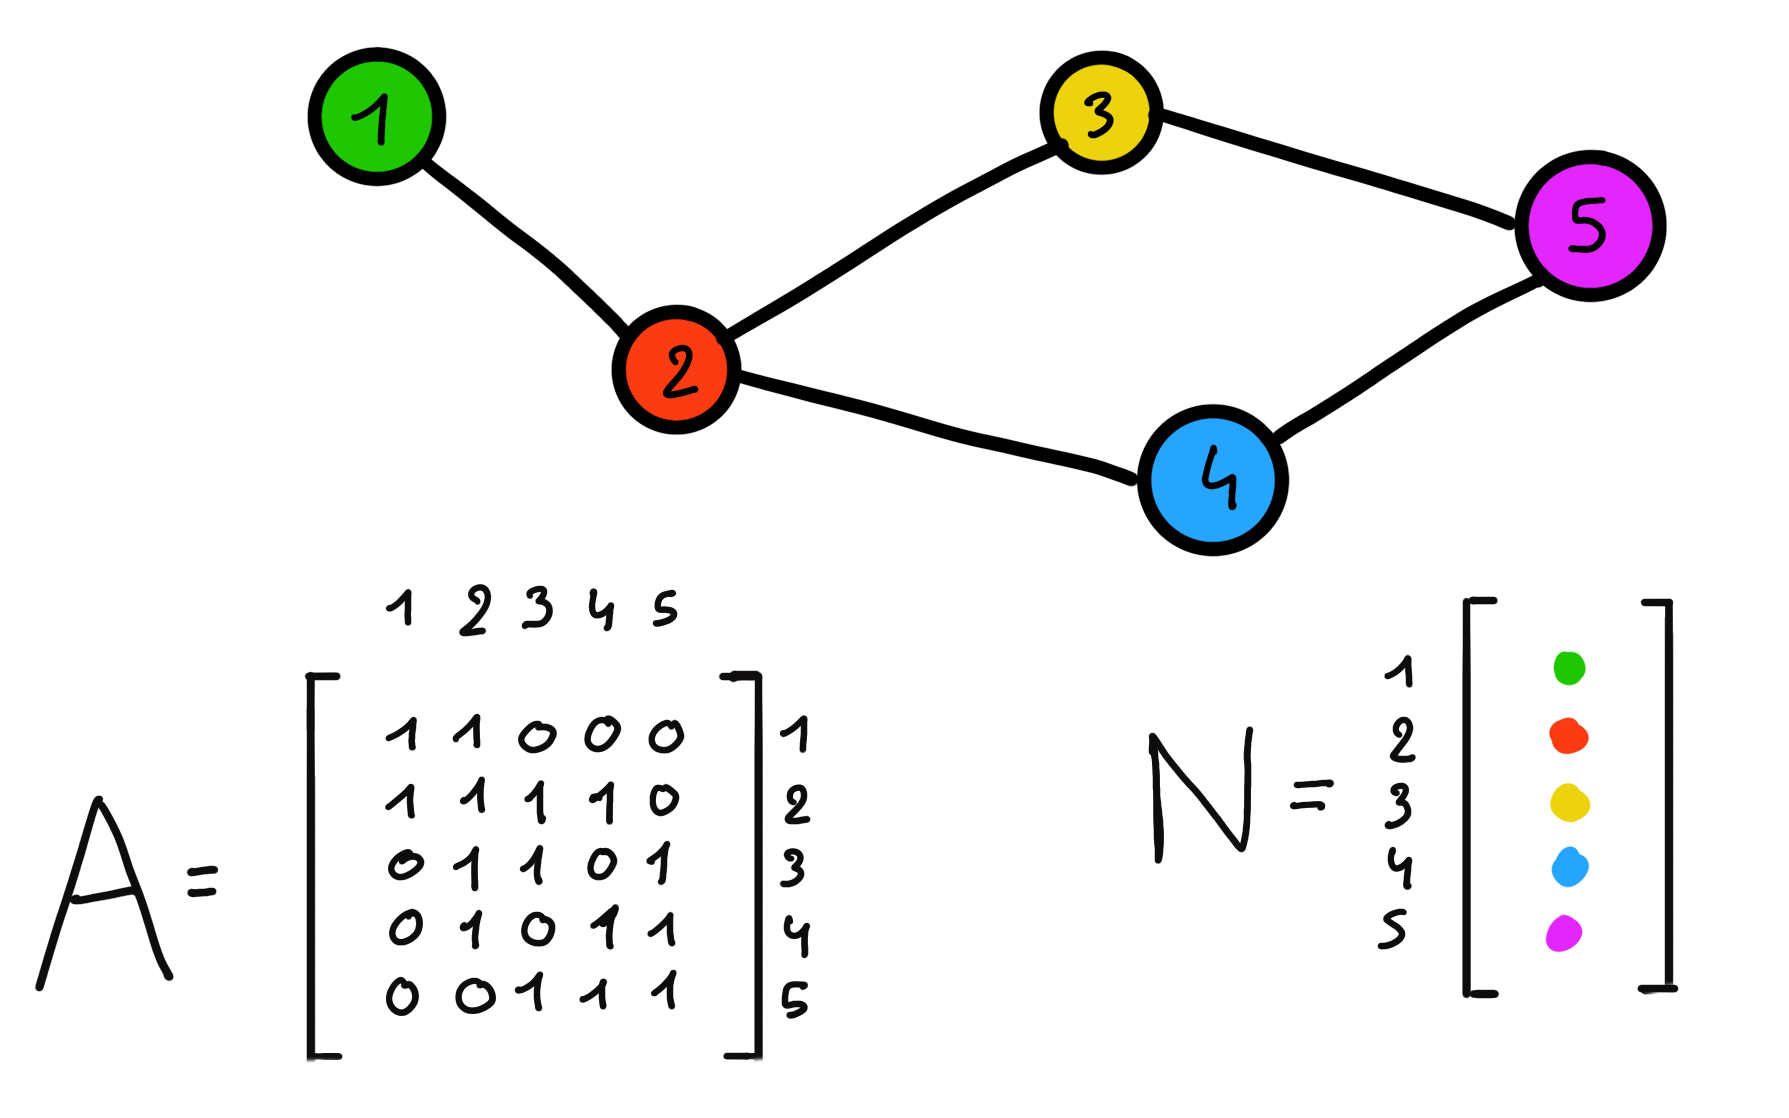
\includegraphics[height=6cm]{images/ml/graph_illustration.png}
  \caption{Illustration of a graph and its tensor representation.}
  \label{fig:ml:gnn:graph}
\end{figure}
A graph $G(\mathcal{N},\mathcal{E})$ is composed of vertex or node $n \in \mathcal{N}$ and edges $e \in \mathcal{E}$. The edges are associated to two nodes $(u, v) \in \mathcal{N}^2$, ``connecting'' them. The node and the edges can hold features, commonly represented as vector $n \in \mathbb{R}^{k_{n}}$, $e \in \mathbb{R}^{k_{e}}$ with $k_n$ and $k_e$ the number of features on the nodes and edges respectively. We can thus define a graph using two tensors $A^{ij}_{\epsilon}$ the adjacency tensor that hold the features $\epsilon \in [0, k_e]$ of the edge connecting the node $i$ and $j$ and the tensor $N^{i}_{\nu}$ that hold the features $\nu \in [0, k_n]$ of a node $i$.

More figuratively, using the example in Figure \ref{fig:ml:gnn:graph}, we have a graph of 5 nodes with a color as feature. The edges have no features, we thus encode their existences as 0 or 1. In a realistic examples as JUNO we could represent each PMTs as nodes and the edges between them as their relation such as distance, timing difference, etc... There no strict rules about what is a node or how they should be linked together. This abstraction allow us to represent virtually any type of detector of any geometry.

\begin{figure}[ht]
  \centering
  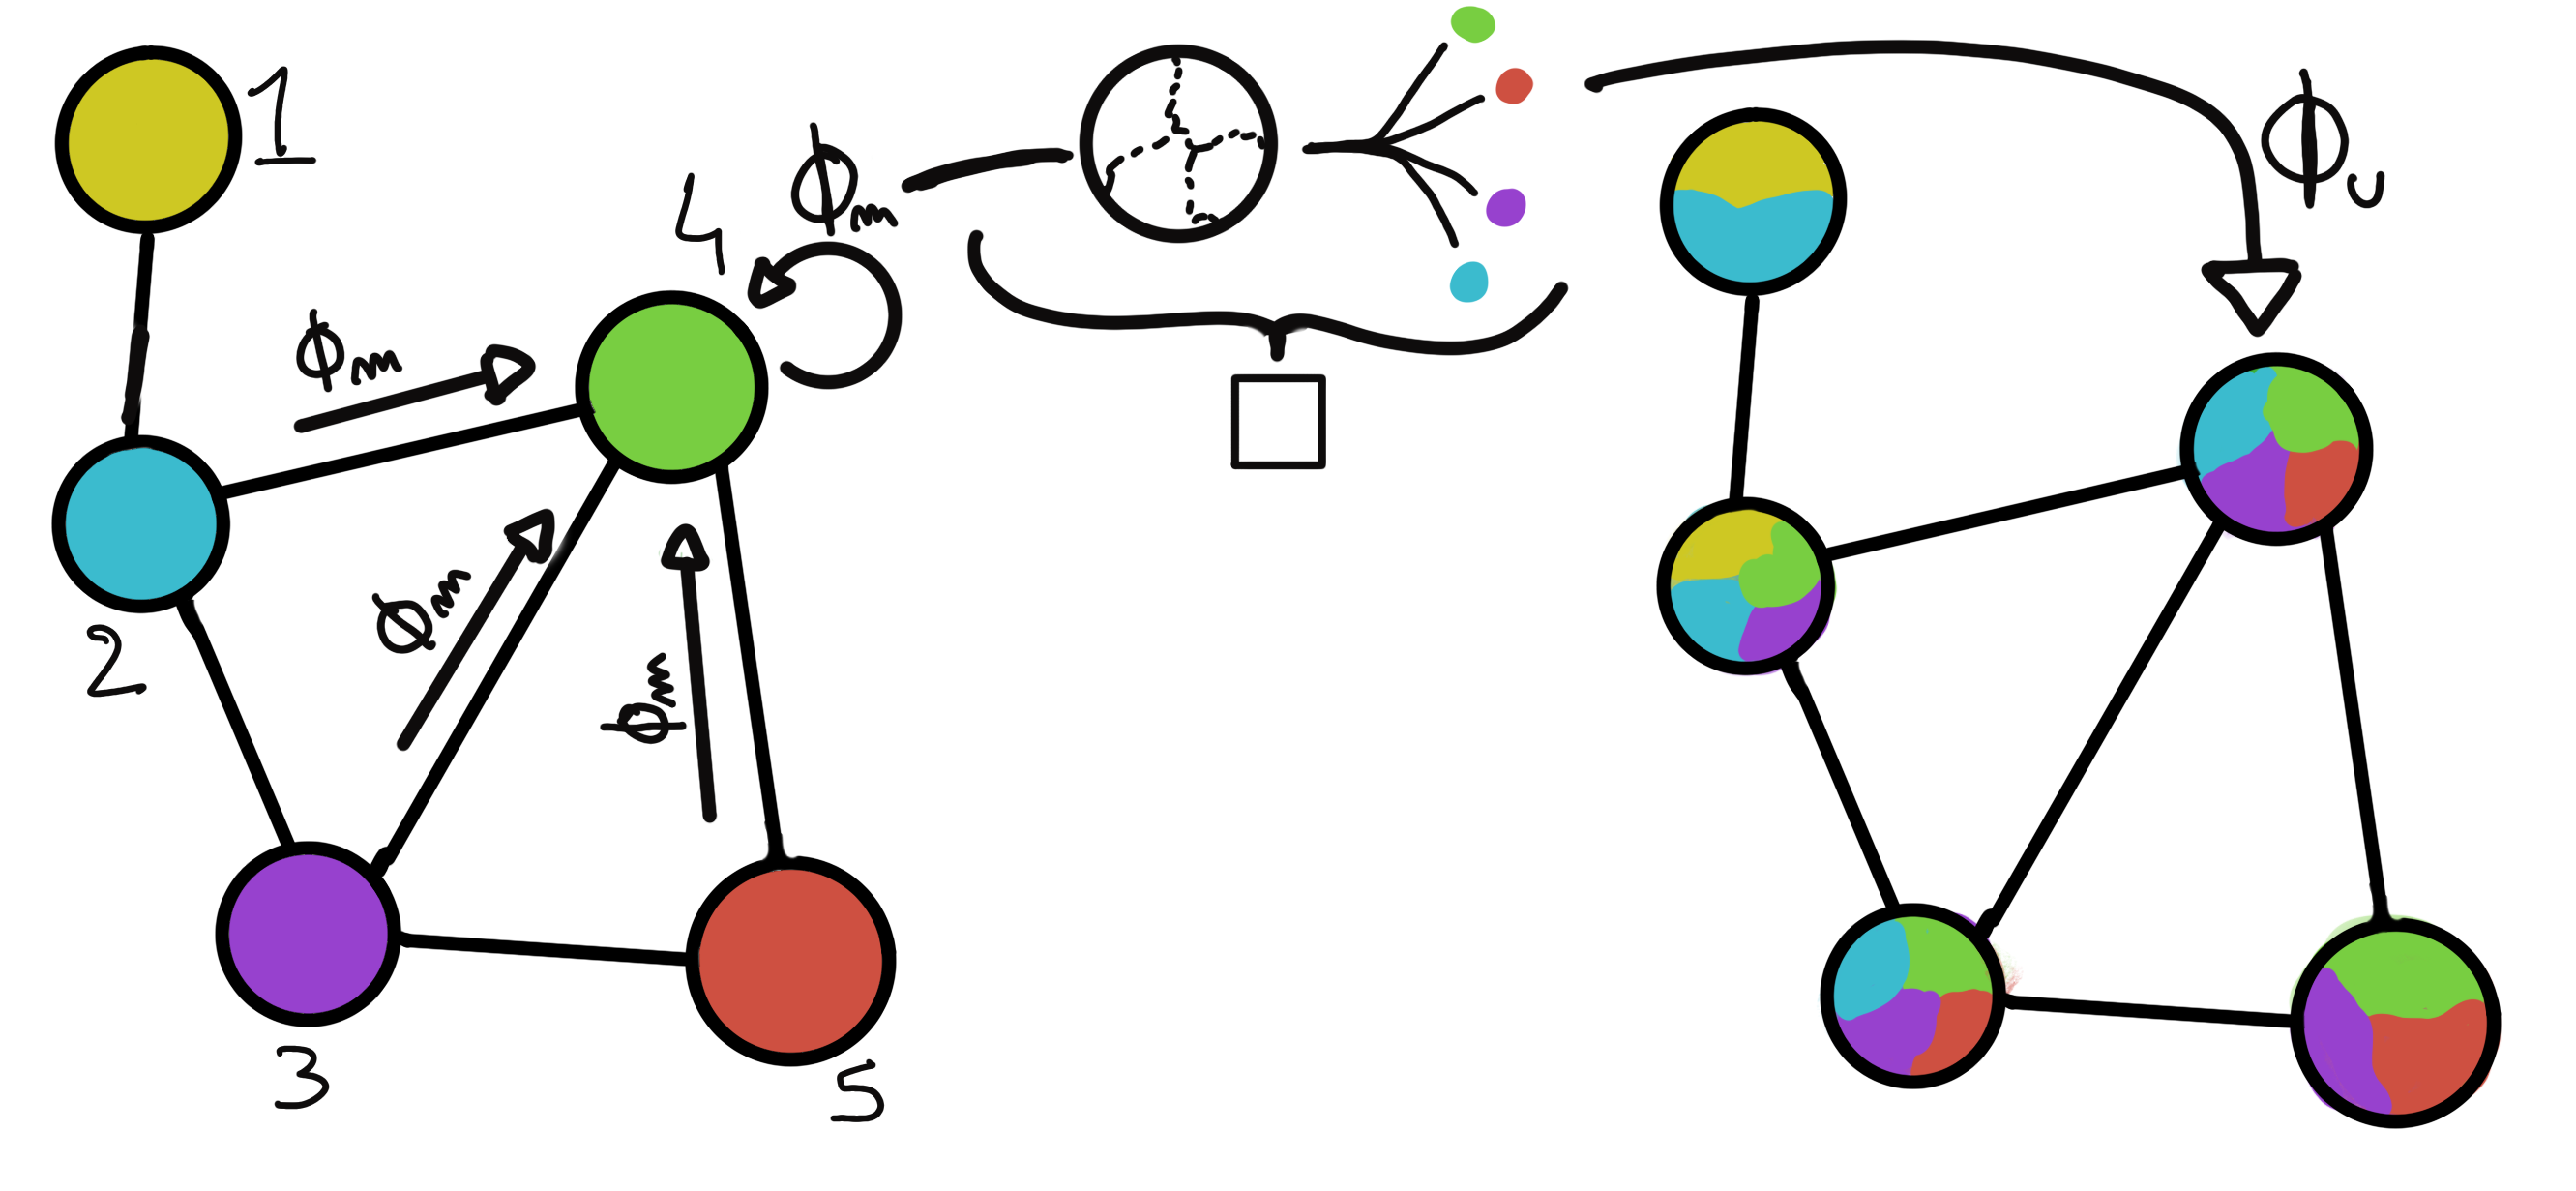
\includegraphics[height=6cm]{images/ml/message_passing.png}
  \caption{Illustration of the message passing algorithm. The detailed explanation can be found in Section \ref{sec:ml:gnn}}
  \label{fig:ml:gnn:message_passing}
\end{figure}

To process such object we need specific machine learning algorithms we call Graph neural network.
To efficiently manipulate graph we need to structurally encode their property in the neural network computing architecture: each node is equivalent (as opposite to ordered data in a vector), each node has a set of neighbours, ... One of this method is the message passing algorithm presented historically in ``Neural Message Passing for Quantum Chemistry'' \cite{gilmer_neural_2017}. In this algorithm, with each layer of message passing a new set of features is computed for each node following
\begin{equation}
  n_i^{k+1} = \phi_u (n_i^k, \Box_j \phi_m(n_i^k, n_j^k, e^k_{ij})); ~ n_j \in \mathcal{N}'_i
\end{equation}
where $\phi_u$ is a differentiable \textit{update} function, $\Box_j$ is a differentiable \textit{aggregation} function and $\phi_m$ is a differentiable \textit{message} function. $\mathcal{N}'_i = \{n_j \in \mathcal{N} | (n_i, n_j) \in \mathcal{E}\}$ is the set of neighbours of $n_i$, i.e. the nodes $n_j$ from which it exist an edge $e_{i,j} \rightarrow (n_i, n_j)$. $k$ is the layer on which the message passing algorithm is applied. The update function need also a few other property if we want to keep the graph property, most notably the permutational invariance of its parameters (example: mean, std, sum, ...). The differents message, update and aggregation functions can really be any kind of function if they follow the constraint presented before, even small Neural Network.

The edges features can also be updated, either by directly taking the results of $\phi_m$ or by using another message function $\phi_e$.

To explain this process, let's take the situation presented in Figure \ref{fig:ml:gnn:message_passing}. We start with an input graph on left, in this case the message passing algorithm is mixing the color on each nodes and produce nodes of mixed color. For simplicity, the $\phi_m$ and $\phi_u$ function are the identity, they take a color and output the same color.

Let's look at what's happening in the node 4. It has 3 neighbours and is a neighbour of itself. The four resulting $\phi_m$ extract the color of each nodes and then feed them to the $\Box$ function. The $\Box$ function just equally distribute the color in the node. Finally the $\phi_u$ function just update the node with the output of $\Box$.

Interestingly we see that the new node 4 does not have any yellow, the color of node 1. But if we were to run the message passing algorithm again, it would get some as node 2 is now partially yellow. If color here represent information, we see that multiple step are needed so that each node is ``aware'' of the informations the other nodes possess.


Message passing is a very generic way of describing the process of GNN and it can be specialized for convolutional filtering \cite{defferrard_convolutional_2017}, diffusion \cite{li_diffusion_2018} and many other specific operation. GNN are used in a wide variety of application such as regression problematics, node classification, edge classification, node and edge prediction, ...


It is a very versatile but complex tool.

\subsection{Adversarial Neural Network (ANN)}

The adversarial machine learning, Adversarial Neural Networks (ANN) in the case of neural network, is a family of unsupervised machine learning algorithms where the learning algorithm (generator) is competing against another algorithm (discriminator). Taking the example of Generative Adversarial Networks, concept initially developed by Goodfellow et al. \cite{goodfellow_generative_2014}, the discriminator goal is to discriminate between data coming from a reference dataset and data produced by the generator.
The generator goal, on the other hand, is to produce data that the discriminator would not be able to differentiate from data from the reference dataset. The expression of duality between the two models is represented in the loss where, at least a part of it, is driven by the results of the discriminator.

\section{State of the art of the Offline IBD reconstruction in JUNO}
\label{sec:juno:reco}

The main reconstruction method currently run in JUNO is OMILREC, a data-driven method based on a likelihood maximization \cite{wu_new_2019, huang_improving_2021} using only the LPMTs. The first step is to reconstruct the interaction vertex from which the energy reconstruction is dependent. It is also necessary for event pairing and classification.

\subsection{Interaction vertex reconstruction}

To start the likelihood maximization, a rough estimation of the vertex and of the event timing is needed. We start by estimating the vertex position using a charge based algorithm.

\subsubsection{Charge based algorithm}

The charge-based algorithm is basically base on the charge-weighted average of the PMT position.

\begin{align}
  \vec{r}_{cb} = a\cdot\frac{\sum_i q_i \cdot \vec{r}_i}{\sum_i q_i}
\end{align}

Where $q_i$ is the reconstructed charge of the pulse of the $i$th PMT and $\vec{r}_i$ is its position. $\vec{r}_0$ is the reconstructed interaction position. $a$ is a scale factor introduced because a weighted average over a 3D sphere is inherently biased. Using calibration we can estimate $a \approx 1.3$ \cite{li_event_2021}. The results in Figure \ref{fig:juno:rec:cbary} shows that the reconstruction is biased from around 15m and further. This is due to the phenomena called ``total reflection area'' or TR Area.

As depicted in the Figure \ref{fig:juno:rec:refl} the optical photons, given that they have a sufficiently large incidence angle, can be deviated of their trajectories when passing through the interfaces LS-acrylic and water-acrylic due to the optical index difference. This cause photons to be lost or to be detected by PMT further than anticipated if we consider their rectilinear trajectories. This cause the charge barycenter the be located closer to the center than the event really is.

\begin{figure}[ht]
  \begin{subfigure}[t]{0.48\textwidth}
    \centering
    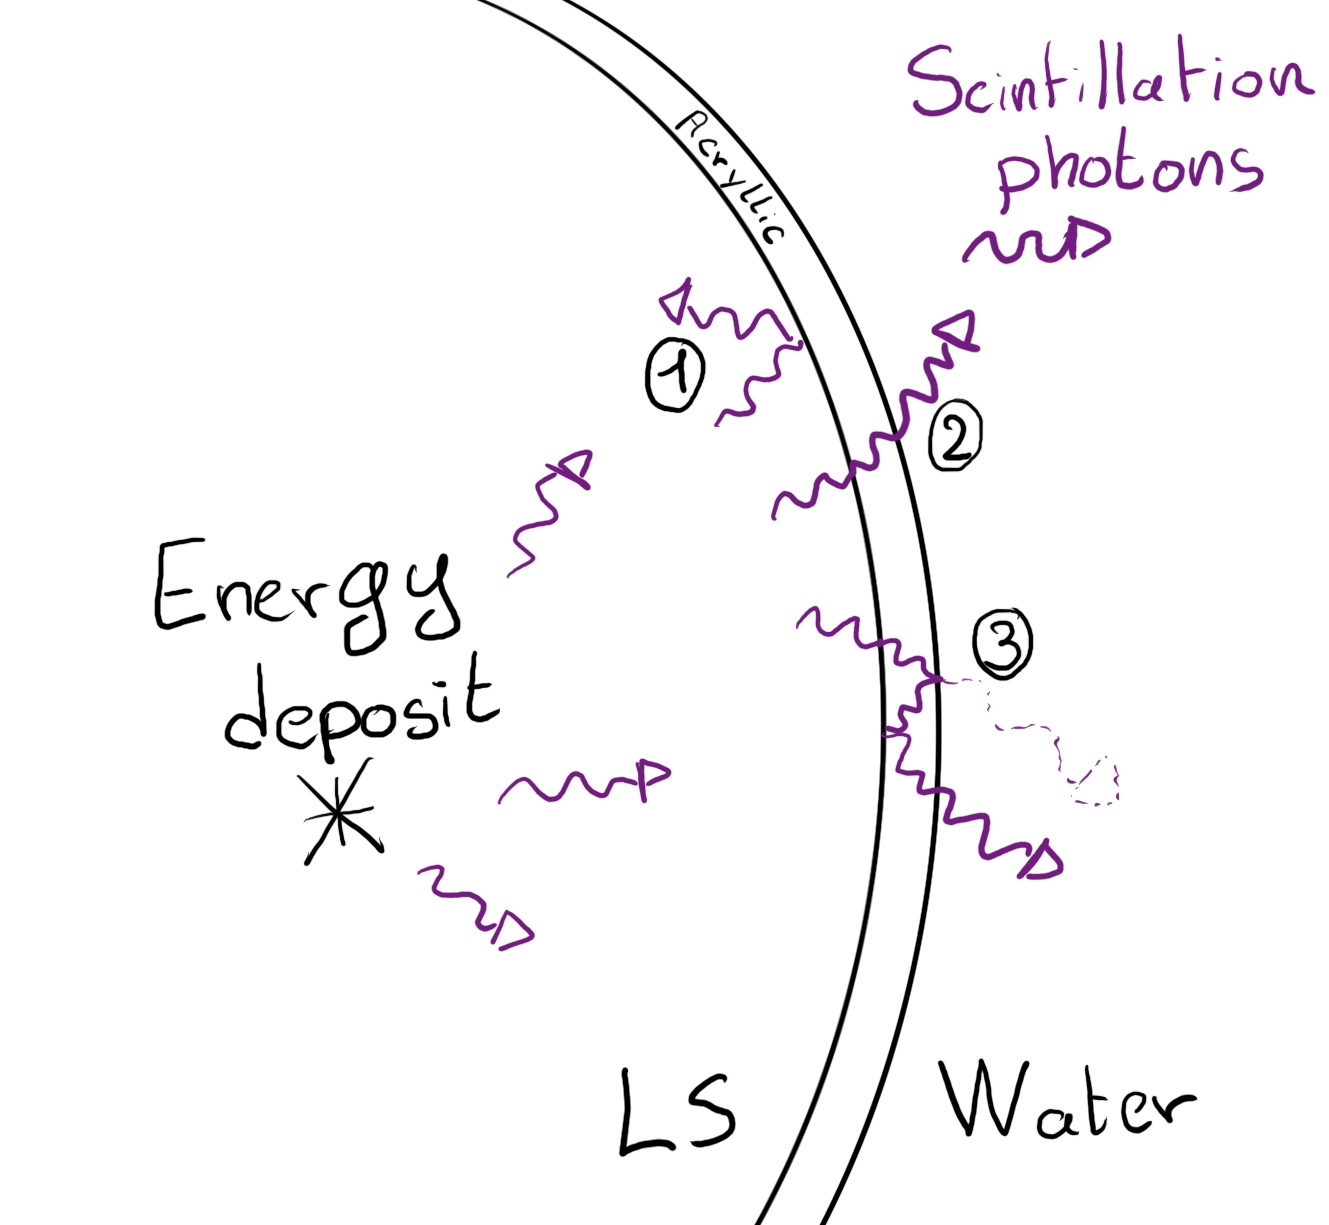
\includegraphics[height=6cm]{images/juno/reco/Reflexion_scenarii.jpg}
    \caption{Illustration of the different optical photons reflection scenarios. \textbf{1} is the reflection of the photon at the interface LS-acrylic or acrylic-water. \textbf{2} is the transmission of the photons through the interfaces. \textbf{3} is the conduction of the photon in the acrylic.}
    \label{fig:juno:rec:refl}
  \end{subfigure}
  \hfill
  \begin{subfigure}[t]{0.48\textwidth}
    \centering
    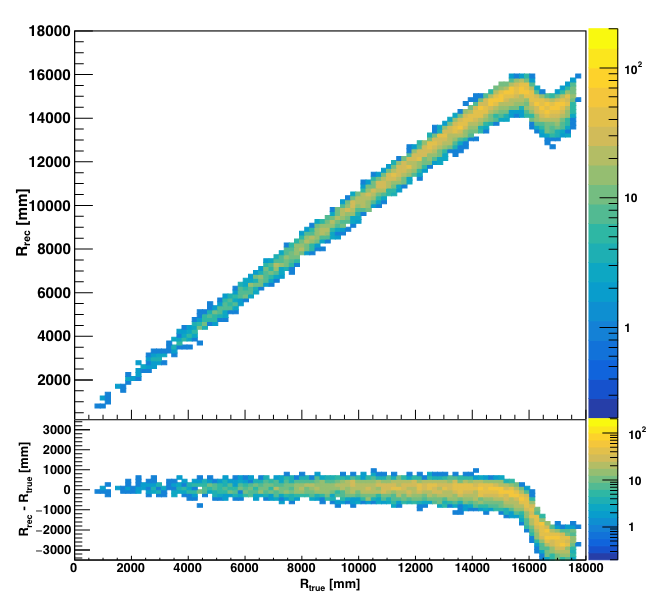
\includegraphics[height=6cm]{images/juno/reco/charge_barycenter.png}
    \caption{Heatmap of $R_{rec}$ and $R_{rec} - R_{true}$ as a function of $R_{true}$ for 4MeV prompt signals uniformly distributed in the detector calculated by the charge based algorithm}
    \label{fig:juno:rec:cbary}
  \end{subfigure}
  \caption{}
\end{figure}

It is to be noted that charge based algorithm, in addition to be biased near the edge of the detector, does not provide any information about the timing of the event. Therefore, a time based algorithm needs to be introduced to provide initial values.

\subsubsection{Time based algorithm}

The time based algorithm use the distribution of the time of flight corrections $\Delta t$ (Eq \ref{eq:juno:rec:tof_corr}) of an event to reconstruct its vertex and $t_0$. It follow the following iterations:

\begin{enumerate}
  \item Use the charge based algorithm to get an initial vertex to start the iteration.

  \item \label{alg:rec:tba} Calculate the time of flight correction for the $i$th PMT using \begin{equation}
      \label{eq:juno:rec:tof_corr}
      \Delta t_i (j) = t_i - \mathrm{tof}_i (j)
    \end{equation}
    where $j$ is the iteration step, $t_i$ is the timing of the $i$th PMT, and $\mathrm{tof}_i$ is the time-of-flight of the photon considering an rectilinear trajectory and an effective velocity in the LS and water (see \cite{li_event_2021} for detailed description of this effective velocity). Plot the $\Delta t$ distribution and label the peak position as $\Delta t^{\mathrm{peak}}$ (see fig \ref{fig:juno:rec:delta_t_distrib}).

  \item Calculate a correction vector $\vec{\delta} [\vec{r}(j)]$ as \begin{equation}
      \vec{\delta} [\vec{r}(j)] = \frac{\sum_i \bigg(\frac{\Delta t(j) - \Delta t^{\mathrm{peak}}(j)}{\mathrm{tof}_i(j)} \bigg) \cdot (\vec{r}_0(j) - \vec{r}_i)}{N^{\mathrm{peak}}(j)}
    \end{equation}
    where $\vec{r}_0$ is the vertex position at the beginning of this iteration, $\vec{r}_i$ is the position of the $i$th PMT. To minimize the effect of scattering, dark noise and reflection, only the pulse happening in a time window (-10 ns, +5 ns) around $\Delta t^{\mathrm{peak}}$ are considered. $N^{\mathrm{peak}}$ is the number of PE collected in this time-window.

  \item if $\vec{\delta} [\vec{r}(j)] < 1 \mathrm{mm}$ or $j \geq 100$, stop the iteration. Otherwise $\vec{r}_0 (j + 1) = \vec{r}_0 (j) + \vec{\delta} [\vec{r}(j)]$ and go to step \ref{alg:rec:tba}.
\end{enumerate}

\begin{figure}
  \begin{subfigure}[t]{0.48\textwidth}
    \centering
    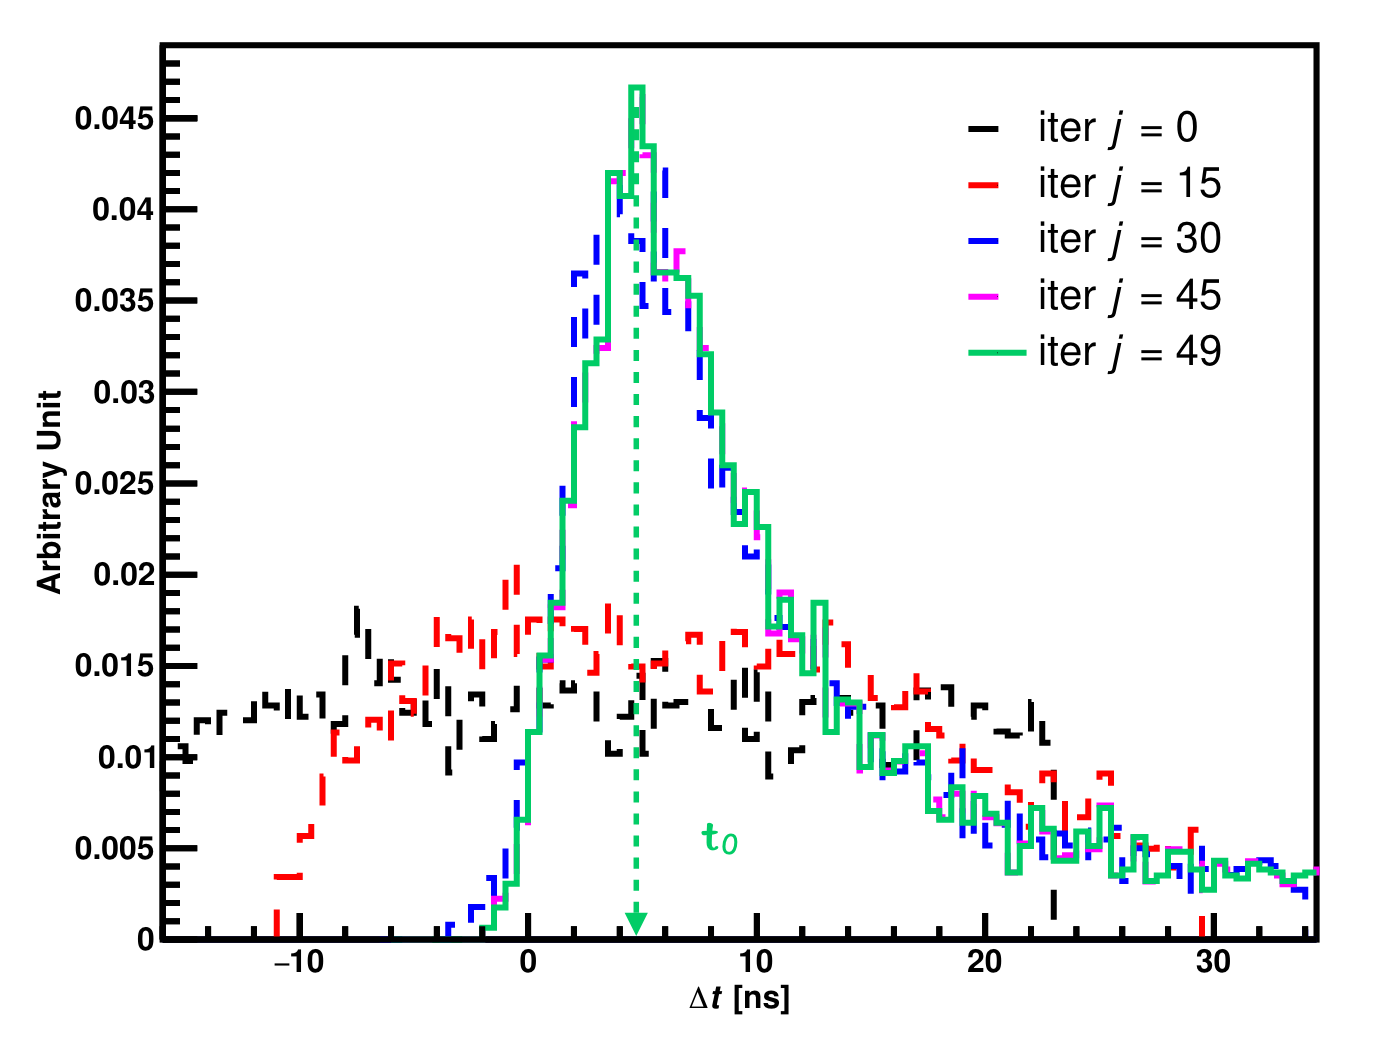
\includegraphics[width=\textwidth]{images/juno/reco/delta_t_peak_distrib.png}
    \caption{$\Delta t$ distribution at different iterations step $j$}
    \label{fig:juno:rec:delta_t_distrib}
  \end{subfigure}
  \hfill
  \begin{subfigure}[t]{0.48\textwidth}
    \centering
    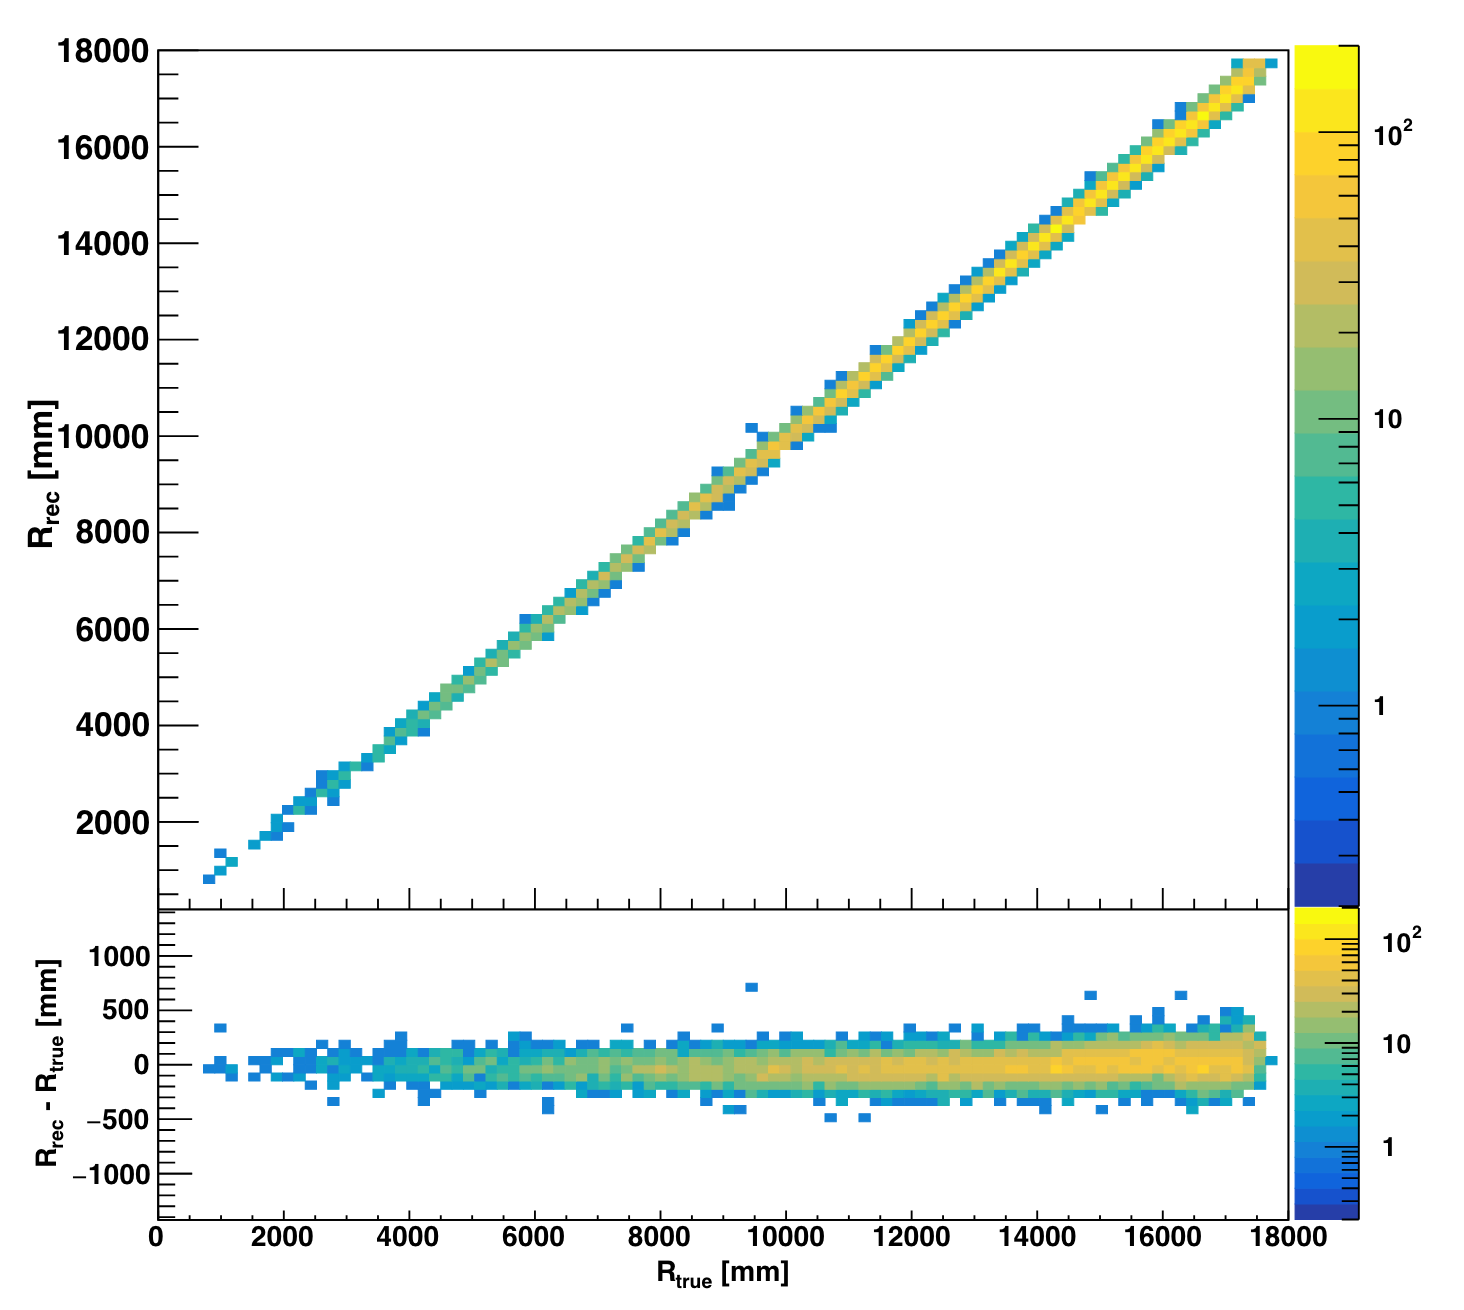
\includegraphics[width=\textwidth]{images/juno/reco/time_based_algorithm.png}
    \caption{Heatmap of $R_{rec}$ and $R_{rec} - R_{true}$ as a function of $R_{true}$ for 4MeV prompt signals uniformly distributed in the detector calculated by the time based algorithm}
    \label{fig:juno:rec:time_based_results}
  \end{subfigure}
  \caption{}
\end{figure}

However because the earliest arrival time is used, $t_i$ is related to the number photoelectrons $N_i^{\mathrm{pe}}$ detected by the PMT \cite{ranucci_analytical_1995, galbiati_time_2006, moszynski_status_1979}. To reduce bias in the vertex reconstruction, the following equation is used to correct $t_i$ into $t'_i$:
\begin{equation}
  t'_{i} = t_i - p_0 / \sqrt{N_i^{\mathrm{pe}}} - p_1 - p_2 / N_i^{\mathrm{pe}}
\end{equation}

The parameters $(p_0, p_1, p_2)$ were optimized to (9.42, 0.74, -4.60) for Hamamatsu PMTs and (41.31, -12.04, -20.02) for NNVT PMTs \cite{li_event_2021}. The results presented in Figure \ref{fig:juno:rec:time_based_results} shows that the time based algorithm provide a more accurate vertex and is unbiased even in the TR area. This results $(\vec{r}_0, t_0)$ is used as initial value for the likelihood algorithm.

\subsubsection{Time likelihood algorithm}

The time likelihood algorithm use the residual time expressed as follow
\begin{equation}
  \label{eq:juno:rec:t_res}
  t_{\mathrm{res}}^i(\vec{r}_0, t_0) = t_i - \mathrm{tof}_i - t_0
\end{equation}

In a first order approximation, the scintillator time response Probability Density Function (PDF) can be described as the emission time profile of the scintillation photons, the Time Transit Spread (TTS) and the dark noise of the PMTs. The emission time profile $f(t_{\mathrm{res}})$ is described like
\begin{equation}
  f(t_{\mathrm{res}}) = \sum_k \frac{\rho_k}{\tau_k} e^{\frac{-t_{\mathrm{res}}}{\tau_k}}, ~ \sum_k \rho_k = 1
\end{equation}
as the sum of the $k$ component that emit light in the LS each one characterised by it's decay time $\tau_k$ and intensity fraction $\rho_k$. The TTS component is expressed as a gaussian convolution
\begin{equation}
  g(t_{\mathrm{res}}) = \frac{1}{\sqrt{2\pi}\sigma}e^{\frac{-(t_{\mathrm{res}} - \nu)^2}{2\sigma^2}} \cdot f(t_{\mathrm{res}})
\end{equation}
where $\sigma$ is the TTS of PMTs and $\nu$ is the average transit time. The dark noise is not correlated with any physical events and considered as constant rate over the time window considered $T$. By normalizing the dark noise probability $\epsilon(t_{\mathrm{res}})$ as $\int_T \epsilon(t_{\mathrm{res}}) dt_{\mathrm{res}} = \epsilon_{\mathrm{dn}}$ , it can be integrated in the PDF as
\begin{equation}
  \label{eq:juno:juno:tim_like:dn}
  p(t_{\mathrm{res}}) = (1-\epsilon_{\mathrm{dn}}) \cdot g(t_{\mathrm{res}}) + \epsilon(t_{\mathrm{res}})
\end{equation}

The distribution of the residual time $t_{\mathrm{res}}$ of an event can then be compared to $p(t_{\mathrm{res}})$ and the best fitting vertex $\vec{r}_0$ and $t_0$ can be chosen by minimizing
\begin{equation}
  \mathcal{L}(\vec{r}_0, t_0) = - \mathrm{ln} \bigg(\prod_i p(t^i_{\mathrm{res}}) \bigg)
\end{equation}

The parameter of Eq. \ref{eq:juno:juno:tim_like:dn} can be measured experimentally. The results shown in Figure \ref{fig:juno:rec:time_likelihood} used PDF from monte carlo simulation. The results shows that $R_{rec} - R_{true}$ is biased depending on the energy. While this could be corrected using calibration, another algorithm based on charge likelihood was developed to correct this problem.

\begin{figure}[ht]
  \centering
  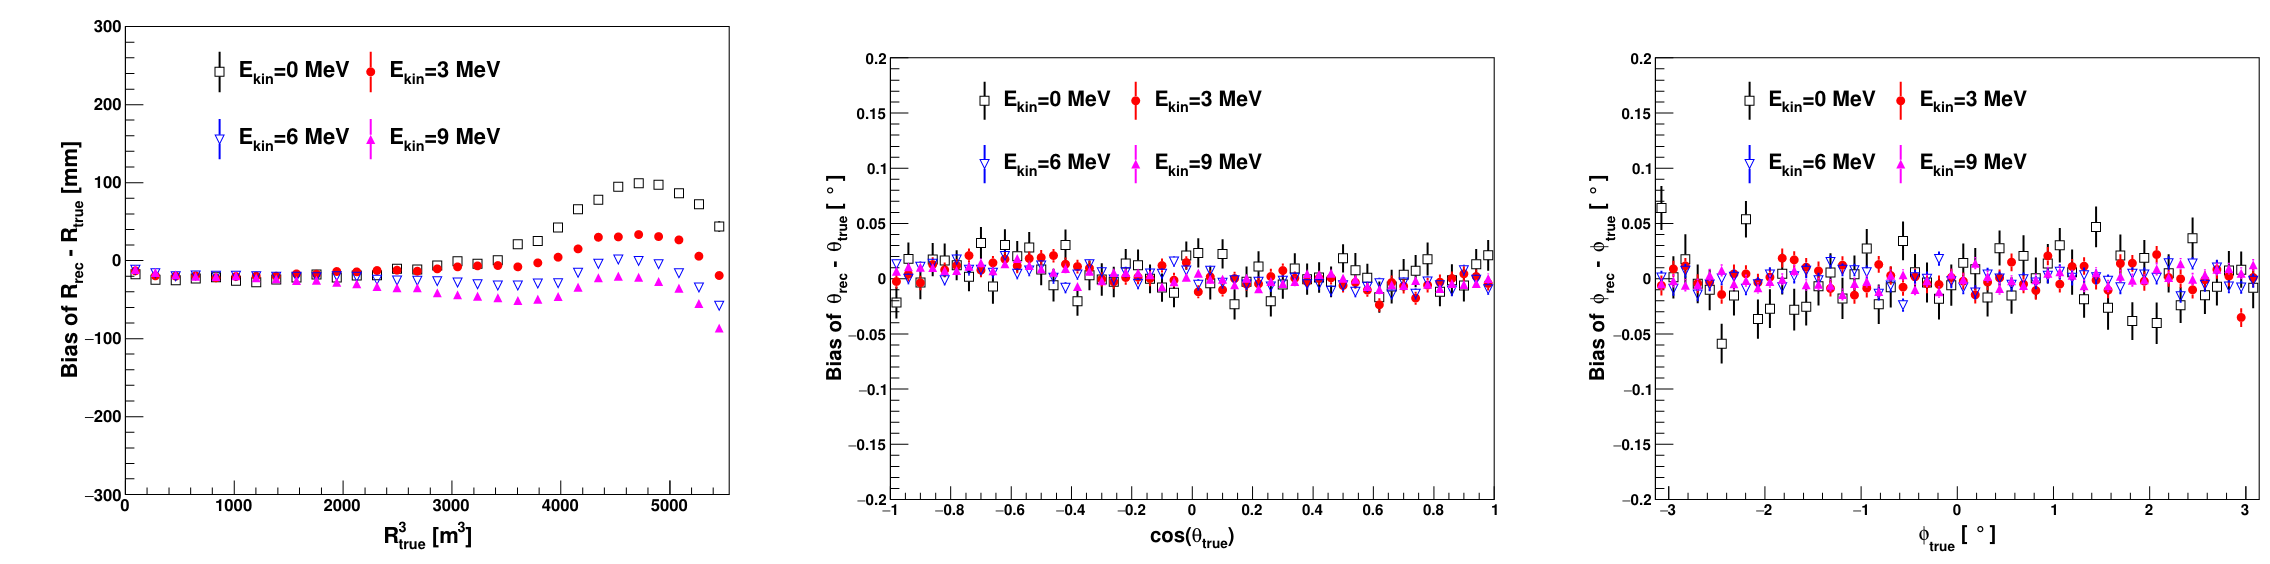
\includegraphics[width=\linewidth]{images/juno/reco/time_likelihood_results.png}
  \caption{Bias of the reconstructed radius R (left), $\theta$ (middle) and $\phi$ (right) for multiple energies by the time likelihood algorithm}
  \label{fig:juno:rec:time_likelihood}
\end{figure}


\subsubsection{Charge likelihood algorithm}

Similarly to the time likelihood algorithms that use a timing PDF, the charge likelihood algorithm use a PE PDF for each PMT depending on the energy and position of the event. With $\mu(\vec{r}_0, E)$ the mean expected number of PE detected by each PMT, the probability to observe $N_{pe}$ in a PMT follow a Poisson distribution. Thus
\begin{itemize}
  \item The probability to observe no hit ($N_{pe} = 0$) in the $j$th PMT is $P^{j}_{nohit} (\vec{r}_0, E) = e^{-\mu_j}$
  \item The probability to observe $N_{pe} \neq 0$ in the $i$th PMT is $P^{i}_{hit} (\vec{r}_0, E) = \frac{\mu^{N^i_{pe}} e^{-\mu_i}}{N^i_{pe}!}$
\end{itemize}

Therefore, the probability to observe a specific hit pattern can be expressed as
\begin{equation}
  P(\vec{r}_0, E) = \prod_j P^j_{nohit}(\vec{r}_0, E) \cdot \prod_i P^i_{hit}(\vec{r}_0, E)
\end{equation}

The best fit values of $\vec{R}_0$ and $E$ can then be calculated by minimizing the negative log-likelihood
\begin{equation}
  \label{eq:juno:rec:charge_likelihood}
  \mathcal{L}(\vec{r}_0, E) = - \mathrm{ln}(P(\vec{r}_0,E))
\end{equation}

In principle, $\mu_i(\vec{r}_0, E)$ could be expressed
\begin{equation}
  \label{eq:juno:rec:mu_i}
  \mu_i(\vec{r}_0, E) = Y \cdot \frac{\Omega(\vec{r}_0, r_i)}{4 \pi} \cdot \epsilon_i \cdot f(\theta_i) \cdot e^{-\sum_m \frac{d_m}{\zeta_m}}\cdot E + \delta_i
\end{equation}
where $Y$ is the energy scale factor, $\Omega(\vec{r}_0, r_i)$ is the solid angle of the $i$th PMT, $\epsilon_i$ is its detection efficiency, $f(\theta_i)$ its angular response, $\zeta_m$ is the attenuation length in the materials and $\delta_i$ the expected number of dark noise.

However Eq. \ref{eq:juno:rec:mu_i} assume that the scintillation light yield is linear with energy and describe poorly the contribution of indirect light, shadow effect due to the supporting structure and the total reflection effects. The solution is to use data driven methods to produce the pdf by using the calibrations sources and position described in Section \ref{sec:juno:calib}. In the results presented in Figures \ref{fig:juno:rec:time_charge_results}, the PDF was produced using MC simulation and 29 specific calibrations position \cite{li_event_2021} along the Z-axis of the detector.
\begin{figure}[ht]
  \centering
  \begin{subfigure}[b]{0.48\linewidth}
    \centering
    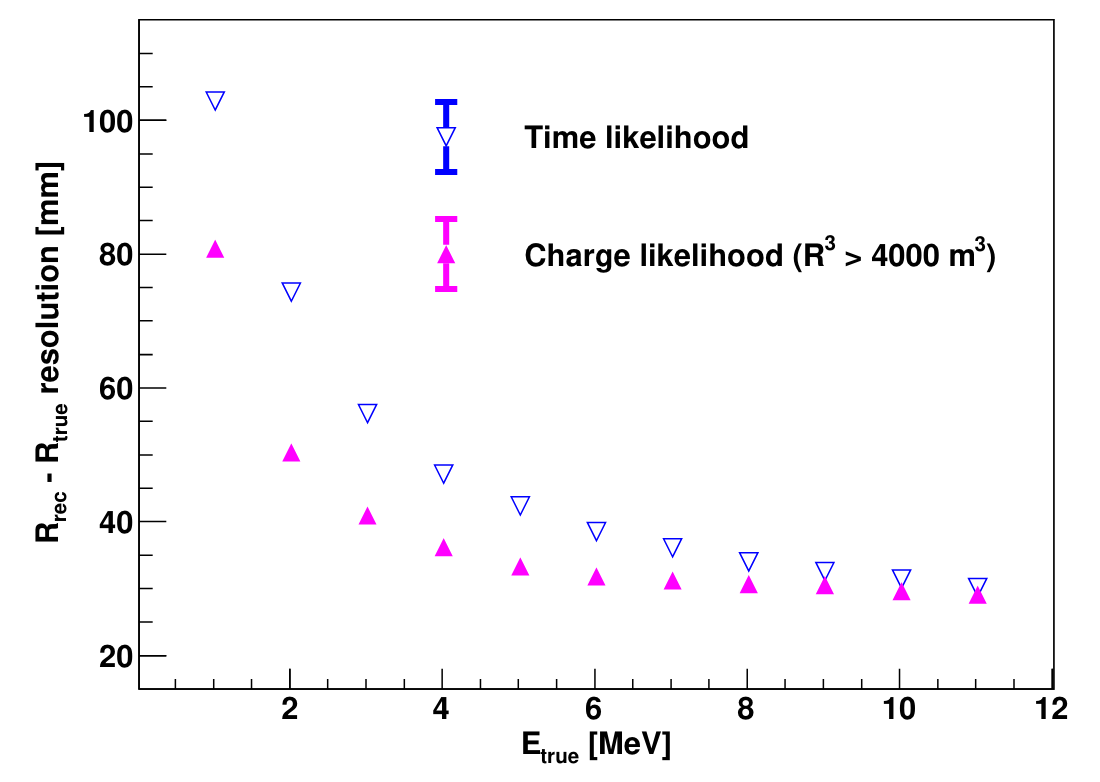
\includegraphics[width=\textwidth]{images/juno/reco/charge_likelihood_res.png}
  \end{subfigure}
  \hfill
  \begin{subfigure}[b]{0.48\linewidth}
    \centering
    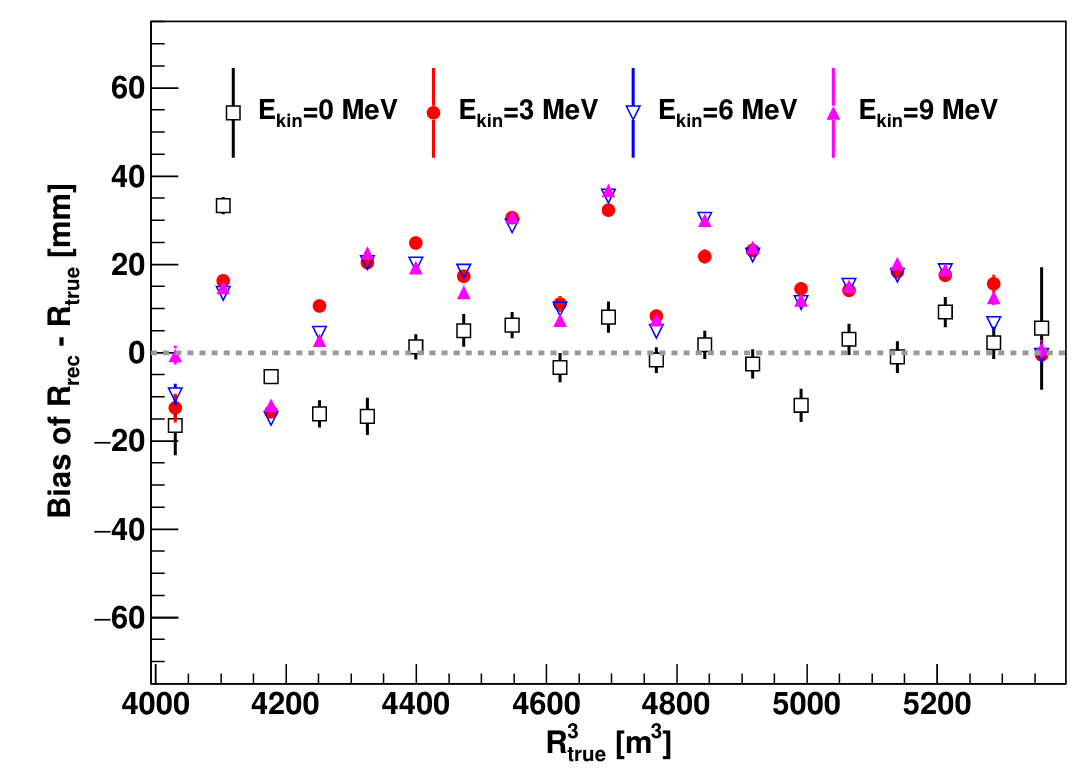
\includegraphics[width=\textwidth]{images/juno/reco/charge_likelihood_bias.png}
  \end{subfigure}
  \caption{\textbf{On the left:} Resolution of the reconstructed R as a function of the energy in the TR area ($R^3 > 4000 \mathrm{m}^3 \equiv R > 16 m$) by the charge and time likelihood algorithms. \textbf{On the right:} Bias of the reconstructed R in the TR area for different energies by the charge likelihood algorithm}
  \label{fig:juno:rec:time_charge_results}
\end{figure}
We see that the charge likelihood algorithm show little bias in the TR area and a better resolution than the time likelihood. The Figure \ref{fig:juno:rec:all_class} shows the radial resolution of the different algorithm presented for this section, we can see the refinement at each step and that the charge likelihood yield the best results.

\begin{figure}[ht]
  \centering
  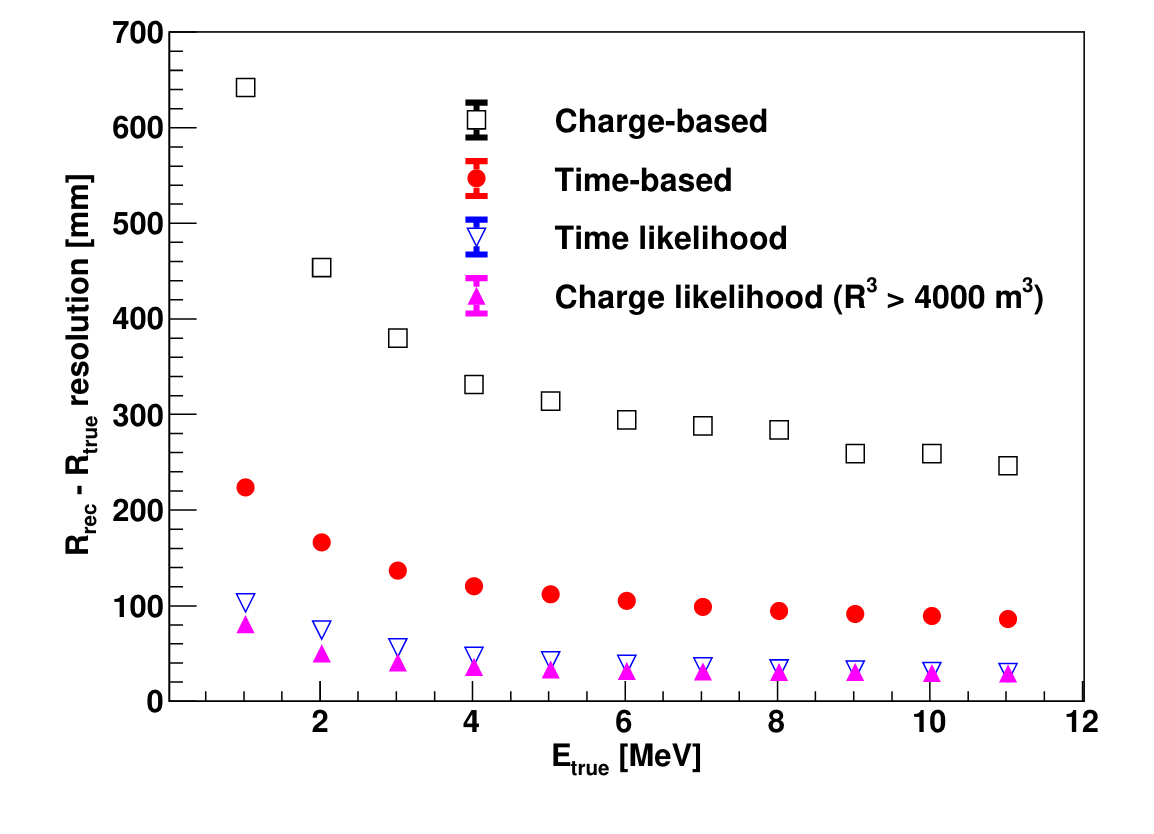
\includegraphics[height=6cm]{images/juno/reco/vertex_reco_classique.png}
  \caption{Radial resolution of the different vertex reconstruction algorithms as a function of the energy}
  \label{fig:juno:rec:all_class}
\end{figure}

The charge based likelihood algorithms already give use some information on the energy as Eq. \ref{eq:juno:rec:charge_likelihood} is minimized but the energy can be further refined as shown in the next section.


\subsection{Energy reconstruction}

As explained in Section \ref{sec:juno:nom_precise_measurement}, energy resolution is crucial for the NMO and oscillation parameters measurements. Thus the energy reconstruction algorithm should take into consideration as much detector effect as possible. The following method is a data driven method based on calibration samples inspired by the charge likelihood algorithm described above \cite{huang_data-driven_2023}.


\begin{figure}[ht]
  \begin{subfigure}[b]{0.48\linewidth}
    \centering
    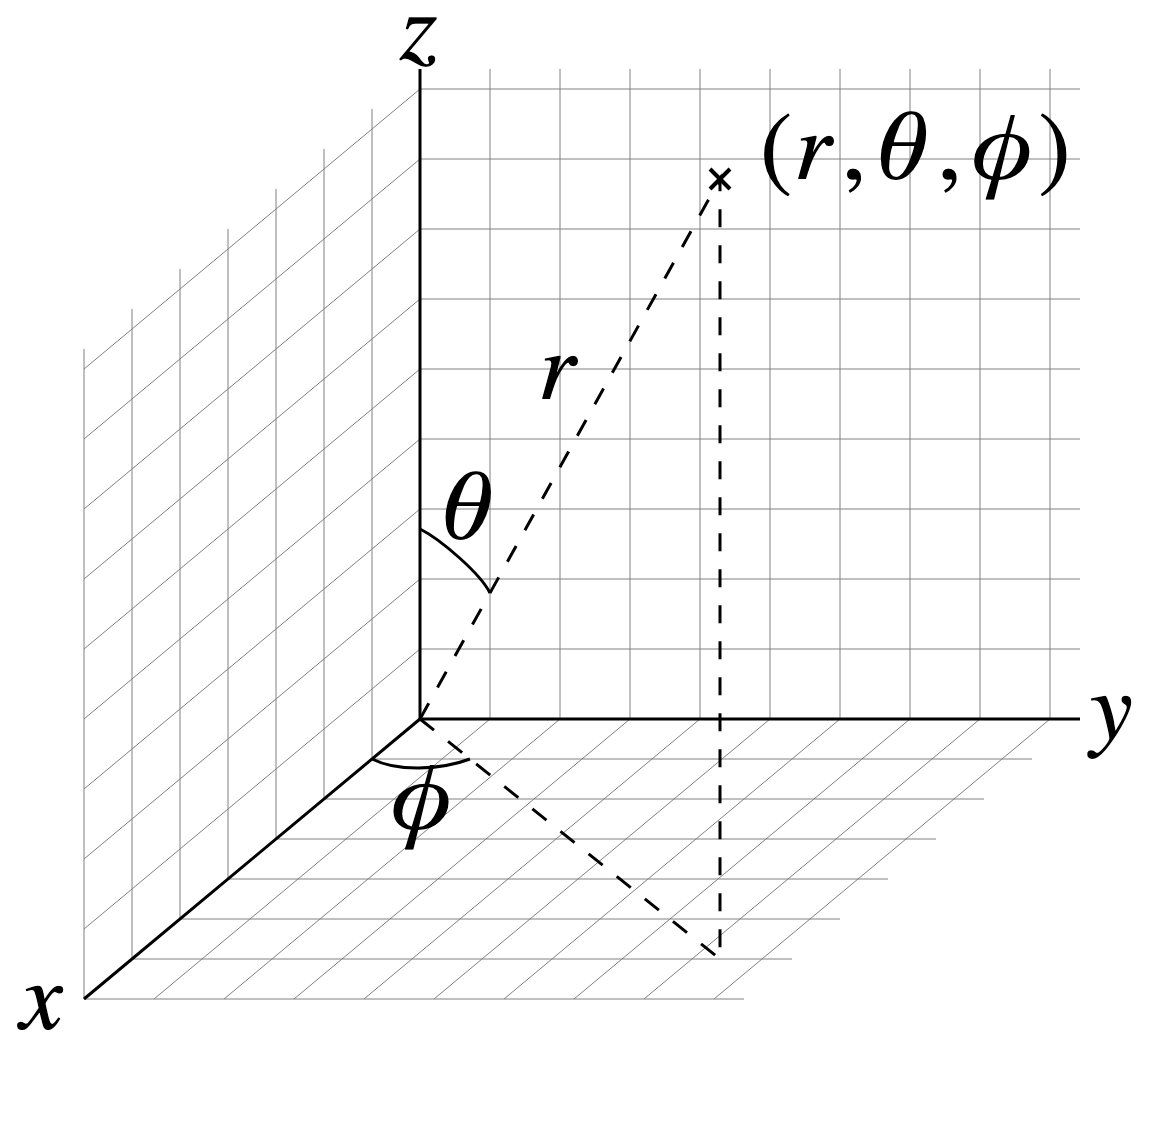
\includegraphics[height=6cm]{images/juno/spherical_coordinate_system.png}
    \caption{Spherical coordinate system used in JUNO for reconstruction}
    \label{fig:juno:rec:corrdinate_system}
  \end{subfigure}
  \hfill
  \begin{subfigure}[b]{0.48\linewidth}
    \centering
    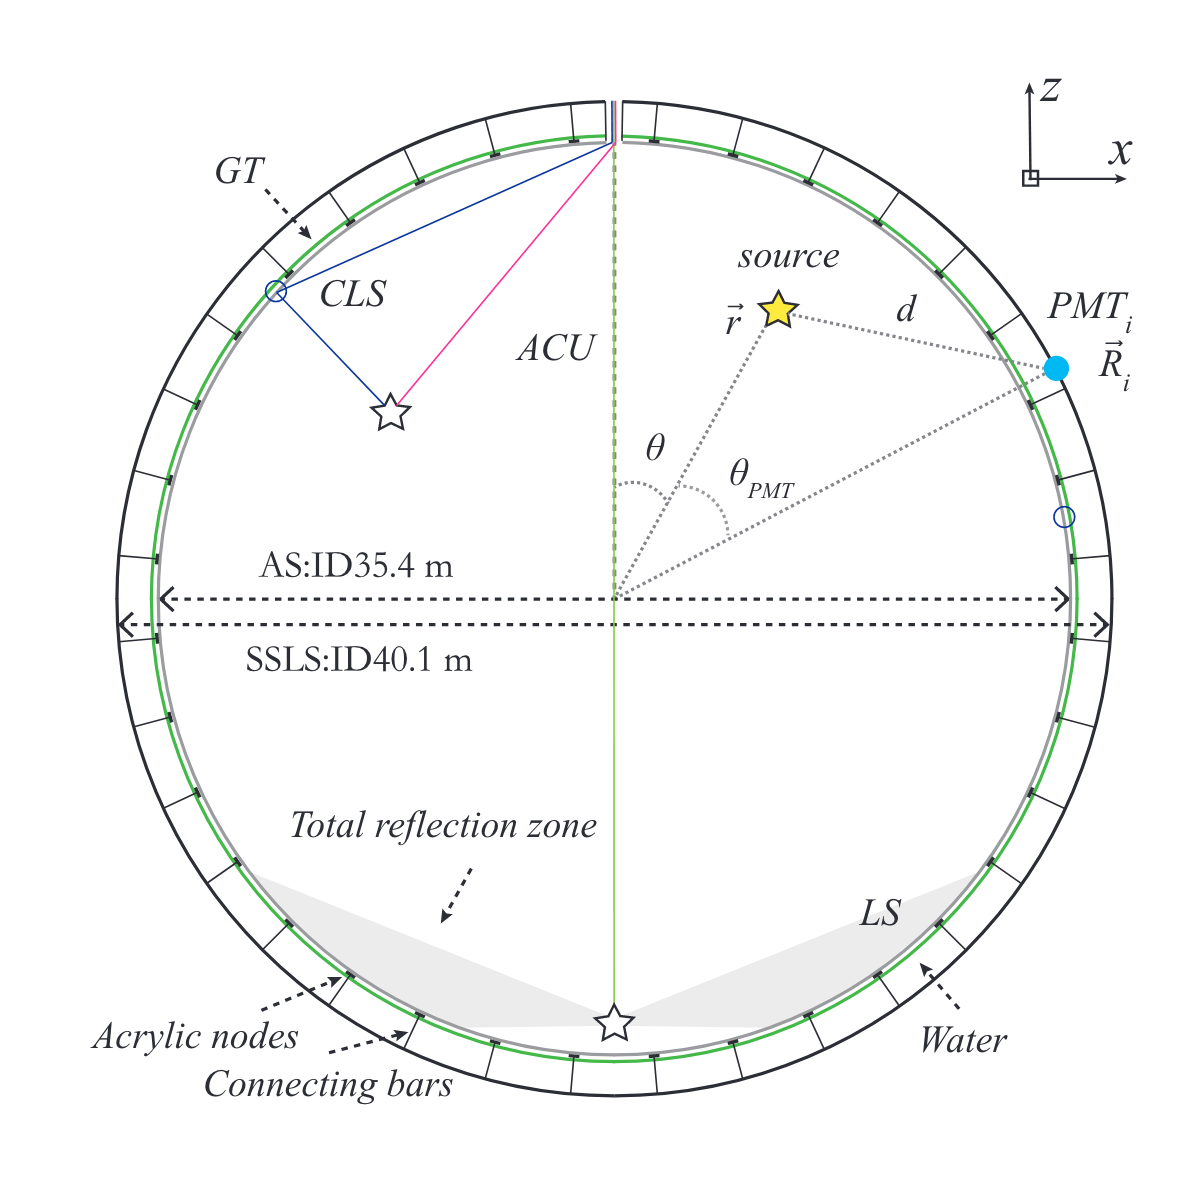
\includegraphics[height=6cm]{images/juno/reco/energy_reco_vars.png}
    \caption{Definition of the variables used in the energy reconstruction}
    \label{fig:juno:rec:energy_vars}
  \end{subfigure}
  \caption{}
\end{figure}

\subsubsection{Charge estimation}

The most important element in the energy reconstruction is $\mu_i(\vec{r}_0, E)$ described in Eq. \ref{eq:juno:rec:mu_i}. For realistic cases, we also need to take into account the electronics effect that were omitted in the previous section. Those effect will cause a charge smearing due to the uncertainties in the $N_{pe}$ reconstruction. Thus we define $\hat{\mu}^L(\vec{r}_0, E)$ which is the expected $N_{pe}/E$ in the whole detector for an event with visible energy $E_{vis}$ and position $\vec{r}_0$. The position of the event and PMTs are now defined using $(r, \theta, \theta_{pmt})$ as defined in Figure \ref{fig:juno:rec:energy_vars}.
\begin{equation}
  \label{eq:juno:reco:charge_est}
  \hat{\mu}(r, \theta, \theta_{pmt}, E_{vis}) = \frac{1}{E_{vis}} \frac{1}{M} \sum_i^M\frac{\frac{\bar{q}_i}{\hat{Q}_i} - \mu_i^D}{\mathrm{DE}_i}, ~ \mu_i^D = \mathrm{DNR}_i \cdot L
\end{equation}
where $i$ runs over the PMTs with the same $\theta_{pmt}$, $\mathrm{DE}_i$ is the detection efficiency of the $i$th PMT. $\mu_i^D$ is the expected number of dark noise photoelectrons in the time window $L$. The time window have been optimized to $L = 280 ~ \mathrm{ns}$ \cite{huang_data-driven_2023}. $\bar{q}_i$ is the average recorded photoelectrons in the time window and $\hat{Q}_i$ is the expected average charge for 1 photoelectron. The $N_{pe}$ map is constructed following the procedure described in \cite{huang_improving_2021}.

\subsubsection{Time estimation}

The second important observable is the hit time of photons that was previously defined in Eq. \ref{eq:juno:rec:t_res}. It is here refined as
\begin{equation}
  t_r = t_h - \mathrm{tof} - t_0 = t_{LS} + t_{TT}
\end{equation}
where $t_h$ is the time of hit, $t_{LS}$ is the scintillation time and $t_{TT}$ the transit time of PMTs that is described by a gaussian
\begin{equation}
  t_{TT} = \mathcal{N}(\overline{\mu_{TT} + t_{d}}, \sigma_{TT})
\end{equation}
where $\mu_{TT}$ is the mean transit time in PMTs, $\sigma_{TT}$ is the Transit Time Spread (TTS) of the PMTs and $t_{d}$ is the delay time in the electronics. The effective refraction index of the LS is also corrected to take into account the propagation distance in the detector.

The timing PDF $P_T(t_r | r,d,\mu_l,\mu_d,k)$ can now be generated using calibration sources \cite{huang_data-driven_2023}. This PDF describe the probability that the residual time of the first photon hit is in $[t_r, t_r + \delta]$ with $r$ the radius of the event vertex, $d = |\vec{r} - \vec{r}_{PMT}|$ the propagation distance, $\mu_l$ and $\mu_d$ the expected number of PE and dark noise in the electronic reading window and $k$ is the detected number of PE.

Now let denote $f(t, r, d)$ the probability density function of "photoelectron hit a time t" for an event happening at $r$ where the photons traveled the distance $d$ in the LS
\begin{equation}
  F(t, r, d) = \int_t^L f(t', r, d)dt'
\end{equation}
Based on the PDF for one photon $k=1$, one can define
\begin{equation}
  P^l_T(t|k=n) = I^l_n [f_l(t)F^{n-1}_l(t)]
\end{equation}
where the indicator $l$ means that the photons comes from the LS and $I^l_n$ a normalisation factor. To this pdf we add the probability to have photons coming from the dark noise indicated by the indicator $d$ using
\begin{equation}
  f_d(t) = 1 / L, ~ F_d(t) = 1 - \frac{t}{L}
\end{equation}
and so for the case where only one photon is detected by the PMT ($k=1$)
\begin{equation}
  P_T(t|\mu_l, \mu_d, k = 1) = I_1 [ P(1, \mu_l) P(0, \mu_d) f_l(t) + P(0, \mu_l) P(1, \mu_d) f_d(t) ]
\end{equation}
where $P(k_\alpha, \mu_\alpha)$ is the Poisson probability to detect $k_\alpha$ PE from $\alpha \in \{l, d\}$ with the condition $k_l + k_d = k$.

Now that we have the individual timing and charge probability we can construct the charge likelihood referred as QMLE:
\begin{equation}
  \mathcal{L}(q_1, q_2, ..., q_N | \vec{r}, E_{vis}) = \prod_{j \in \mathrm{unfired}} e^{-\mu_j} \prod_{i \in \mathrm{fired}} \bigg(\sum_{k=1} P_Q(q_i|k) \cdot P(k, \mu_i) \bigg)
\end{equation}
where $\mu_i = E_{vis} \hat{\mu_i^L} + \mu_i^D$ and $P(k, \mu_i)$ is the Poisson probability of observing k PE. $P_Q(q_i|k)$ is the charge pdf for $k$ PE. And we can also construct the time likelihood referred as TMLE:
\begin{equation}
  \mathcal{L}(t_{1,r}, t_{2,r}, ..., t_{N,r} | \vec{r}, t_0) = \prod_{i \in \mathrm{hit}} \frac{\sum_{k=1}^K P_T(t_{i,r} | r, d, \mu_i^l, \mu_i^d, k) \cdot P(k, \mu^l_i + \mu^d_i)}{\sum_{k=1}^K P(k, \mu^l_i + \mu^d_i)}
\end{equation}
where $K$ is cut to 20 PE and hit is the set of hits satisfying $-100 < t_{i,r} < 500$ ns.

Merging those two likelihood give the charge-time likelihood QTMLE, the core algorithm of OMILREC.
\begin{equation}
  \mathcal{L}(q_1, q_2, ..., q_N; t_{1,r}, t_{2,r}, ..., t_{N,r} | \vec{r}, t_0 , E_{vis}) = \mathcal{L}(q_1, q_2, ..., q_N | \vec{r}, E_{vis}) \cdot \mathcal{L}(t_{1,r}, t_{2,r}, ..., t_{N,r} | \vec{r}, t_0)
\end{equation}

The radial and energy resolutions of the different likelihood are presented in Figure \ref{fig:juno:rec:qtmle} (from \cite{huang_data-driven_2023}). We can see the improvement of adding the time information to the vertex reconstruction and that an increase in vertex precision can bring improvement in the energy resolution, especially at low energies.

\begin{figure}[ht]
  \begin{subfigure}{0.48\linewidth}
    \centering
    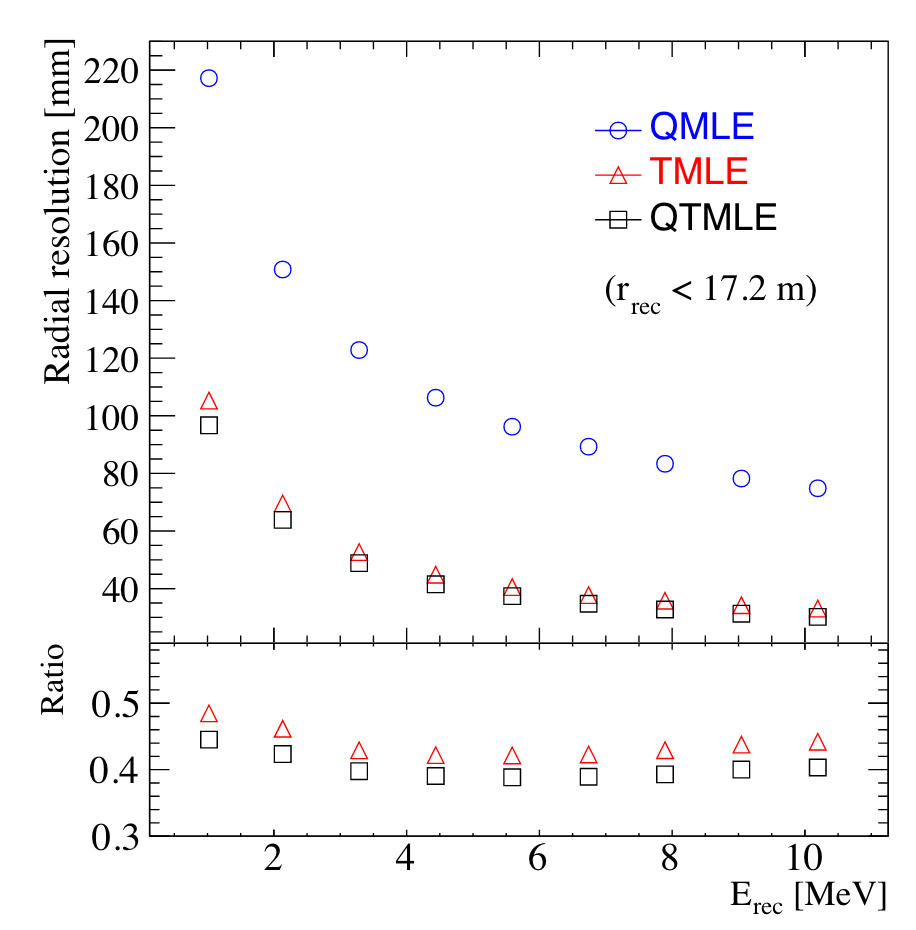
\includegraphics[width=\textwidth]{images/juno/reco/radial_qtmle.png}
    \caption{Radial resolutions of the likelihood-based algorithm TMLE, QMLE and QTMLE}
  \end{subfigure}
  \hfill
  \begin{subfigure}{0.48\linewidth}
    \centering
    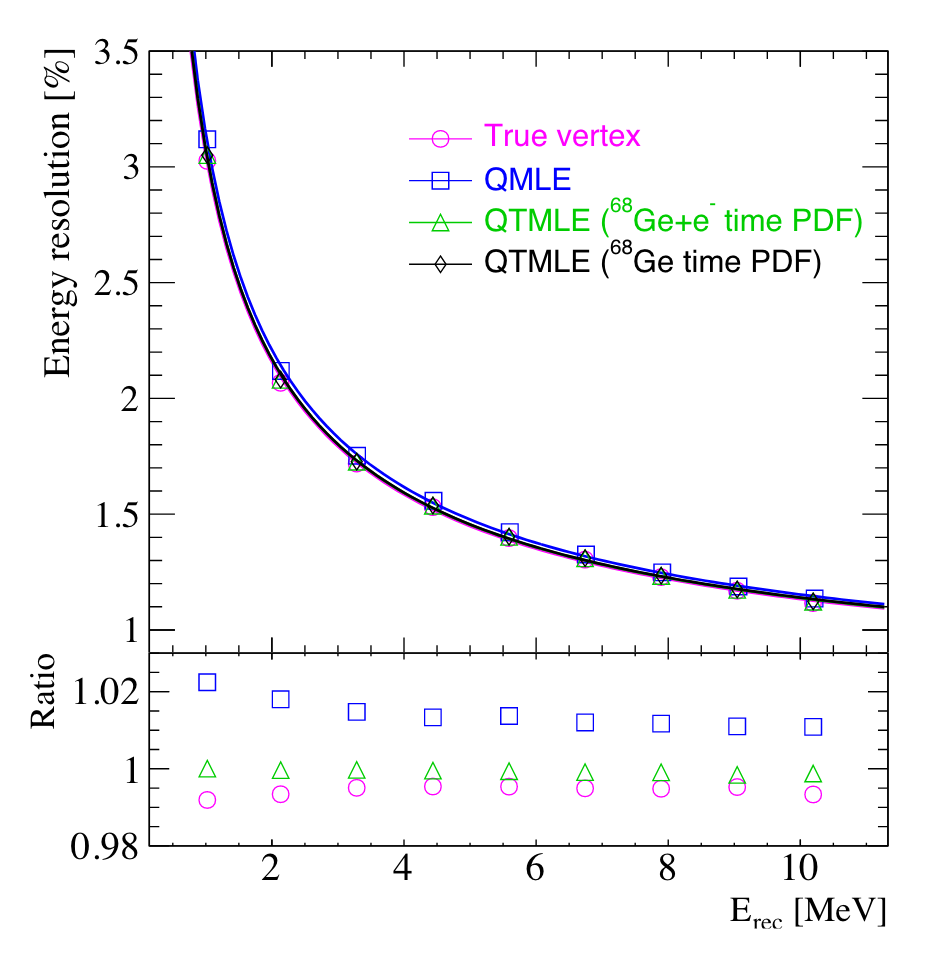
\includegraphics[width=\textwidth]{images/juno/reco/energy_qtmle.png}
    \caption{Energy resolution of QMLE and QTMLE using different vertex resolutions}
  \end{subfigure}
  \caption{}
  \label{fig:juno:rec:qtmle}
\end{figure}

Data driven methods prove to be performant in the energy and vertex reconstruction given that we have enough calibrations sources to produce the PDF. In addition to this, member of JUNO have developed ML algorithms for reconstruction. The one focused on IBD reconstruction are presented in the next section.

\subsection{Machine learning for reconstruction}
\label{sec:juno:ml}

The power of ML is the ability to model complex response to a specific problem. In JUNO the reconstruction problematic can be expressed as follow: knowing that each PMT, large or small, detected a given number of PE $Q$ at a given time $t$ and their position is $x,y,z$ where did the energy was deposited and how much energy was it, modeling a function that naively goes:
\begin{equation}
    \mathbb{R}^{5 \times N_{pmt}} \longmapsto \mathbb{R}^4
\end{equation}
It is worth pointing that while this is already a lot in informations, this is not the rawest representation of the experiment. We could indeed replace the charge and time by the waveform in the time window of the event but that would lead to an input representation size that would exceed our computational limits. Also, due to those computational limits, most of the ML algorithm reduce this input phase space either by structurally encoding the information (pictures, graph), by aggregating it (mean, variance, ...) or by exploiting invariance and equivariance of the experiment (rotational invariance due to the sphericity, ...).

For machine learning to converge to performant algorithm, a large dataset exploring all the phase space of interest is needed. For the following studies, data from the monte carlo simulation presented in Section \ref{sec:juno:software} are used for training. When the detector will be finished calibrations sources will be complementarily be used.

\subsubsection{Boosted Decision Tree (BDT)}

On of the most classic ML method used in physics in last years is the Boosted Decision Tree. They have been explored for vertex reconstruction \cite{qian_vertex_2021} et for energy reconstruction \cite{qian_vertex_2021, gavrikov_energy_2022}.

For vertex and energy reconstruction a BDT was developed using the aggregated informations presented in \ref{tab:juno:rec:bdt_vertex}.

\begin{table}[ht]
  \centering
  \begin{tabular}{l|r}
    Parameter & description \\
    \hline
    $nHits$ & Total number of hits \\
    $x_{cc}, y_{cc}, z_{cc}, R_{cc}$ & Coordinates of the center of charge \\
    $ht_{mean}, ht_{std}$ & Hit time mean and standard deviation
  \end{tabular}
  \caption{Features used by the BDT for vertex reconstruction}
  \label{tab:juno:rec:bdt_vertex}
\end{table}
Its reconstruction performances are presented in Figure \ref{fig:juno:rec:ml_res}.

A second and more advanced BDT, subsequently named BDTE, that only reconstruct energy use a different set of features \cite{gavrikov_energy_2022}. They are presented in the table \ref{tab:juno:rec:bdte}

\begin{table}
  \centering
  \begin{tabular}{|c|c|}
    \hline
    AccumCharge &  $ht_{5\%-2\%}$ \\
    $R_{cht}$ & $pe_{mean}$ \\
    $z_{cc}$ & $J_{cht}$ \\
    $pe_{std}$ & $\phi_{cc}$ \\
    nPMTs &  $ht_{35\%-30\%}$\\
    $ht_{kurtosis}$ & $ht_{20\%-15\%}$ \\
    $ht_{25\%-20\%}$ & $pe_{35\%}$ \\
    $R_{cc}$ & $ht_{30\%-25\%}$ \\
    \hline

  \end{tabular}
  \caption{Features used by the BDTE algorithm. $pe$ and $ht$ reference the charge and hit-time distribution respectively and the percentages are the quantiles of those distributions. $cht$ and $cc$ reference the barycenters of hit time and charge respectively}
  \label{tab:juno:rec:bdte}
\end{table}

\subsubsection{Neural Network (NN)}
Three type of neural networks have explored for event reconstruction in JUNO Deep Neural Network (DNN), Convolutional Neural Network (CNN) and Graph Network (GNN).

The CNN are using 2D projection of the detector representing it as an image with two channel, one for the charge $Q$ and one for the time $t$. The position of the PMTs is structurally encoded in the pixel containing the information of this PMT. In \cite{qian_vertex_2021}, the pixel is chosen based on a transformation of $\theta$ and $\phi$ coordinates to the 2D plane and rounded to the nearest pixel. A sufficiently large image has been chosen to prevent two PMT to be located in the same pixel. An example of this projection can be found in Figure \ref{fig:juno:rec:cnn_proj}. The performances of the CNN can be found in Figure \ref{fig:juno:rec:ml_res}.

\begin{figure}[ht]
  \centering
  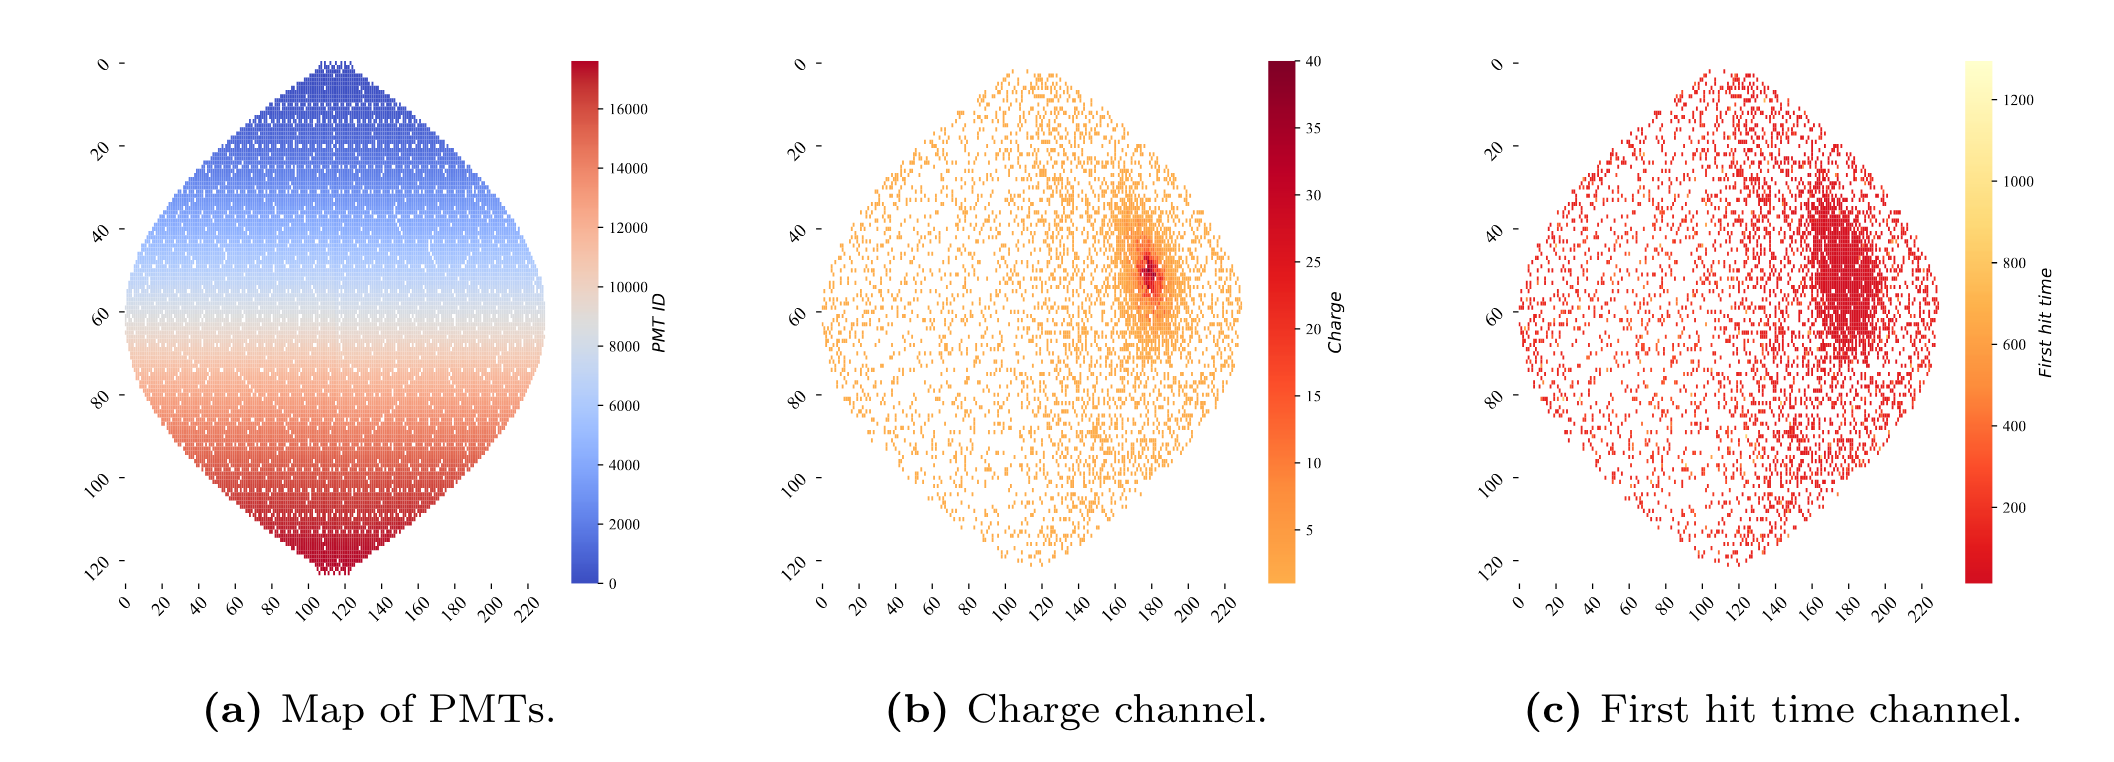
\includegraphics[width=\linewidth]{images/juno/reco/cnn_proj.png}
  \caption{Projection of the LPMTs in JUNO on a 2D plane. (a) Show the distribution of all PMTs and (b) and (c) are example of what the charge and time channel looks like respectively}
  \label{fig:juno:rec:cnn_proj}
\end{figure}

Using 2D have the upside of encoding a large part of the informations structurally but loose the rotational invariance of the detector. It also give undefined information to the neural network (what is a pixel without PMT ? What should be its charge and time ?), cause deformation in the representation of the detector (sides of projection) and loose topological informations.

One of the way to present structurally the sphericity of JUNO to a NN is to use a graph: A collection of objects $V$ called nodes and relations $E$ called edges, each relation associated to a couple ${v_1, v_2}$ forming the graph $G(E, V)$. Nodes and edges can hold informations or features. In \cite{qian_vertex_2021} the nodes, are geometrical region of the detector as defined by the HealPix \cite{gorski_healpix_2005-1}. The features of the nodes are aggregated informations from the PMTs it contains. The edges contains geographic informations of the nodes relative positions.

This data representation has the advantages to keep the topology of the detector intact. It also permit the use of rotational invariant algorithms for the NN, thus taking advantage of the symmetries of the detector.

The neural network then process the graph using Chebyshev Convolutions \cite{defferrard_convolutional_2017}. The performances of the GNN are presented in Figure \ref{fig:juno:rec:ml_res}.


\begin{figure}[ht]
  \centering
  \begin{subfigure}{0.48\linewidth}
    \centering
    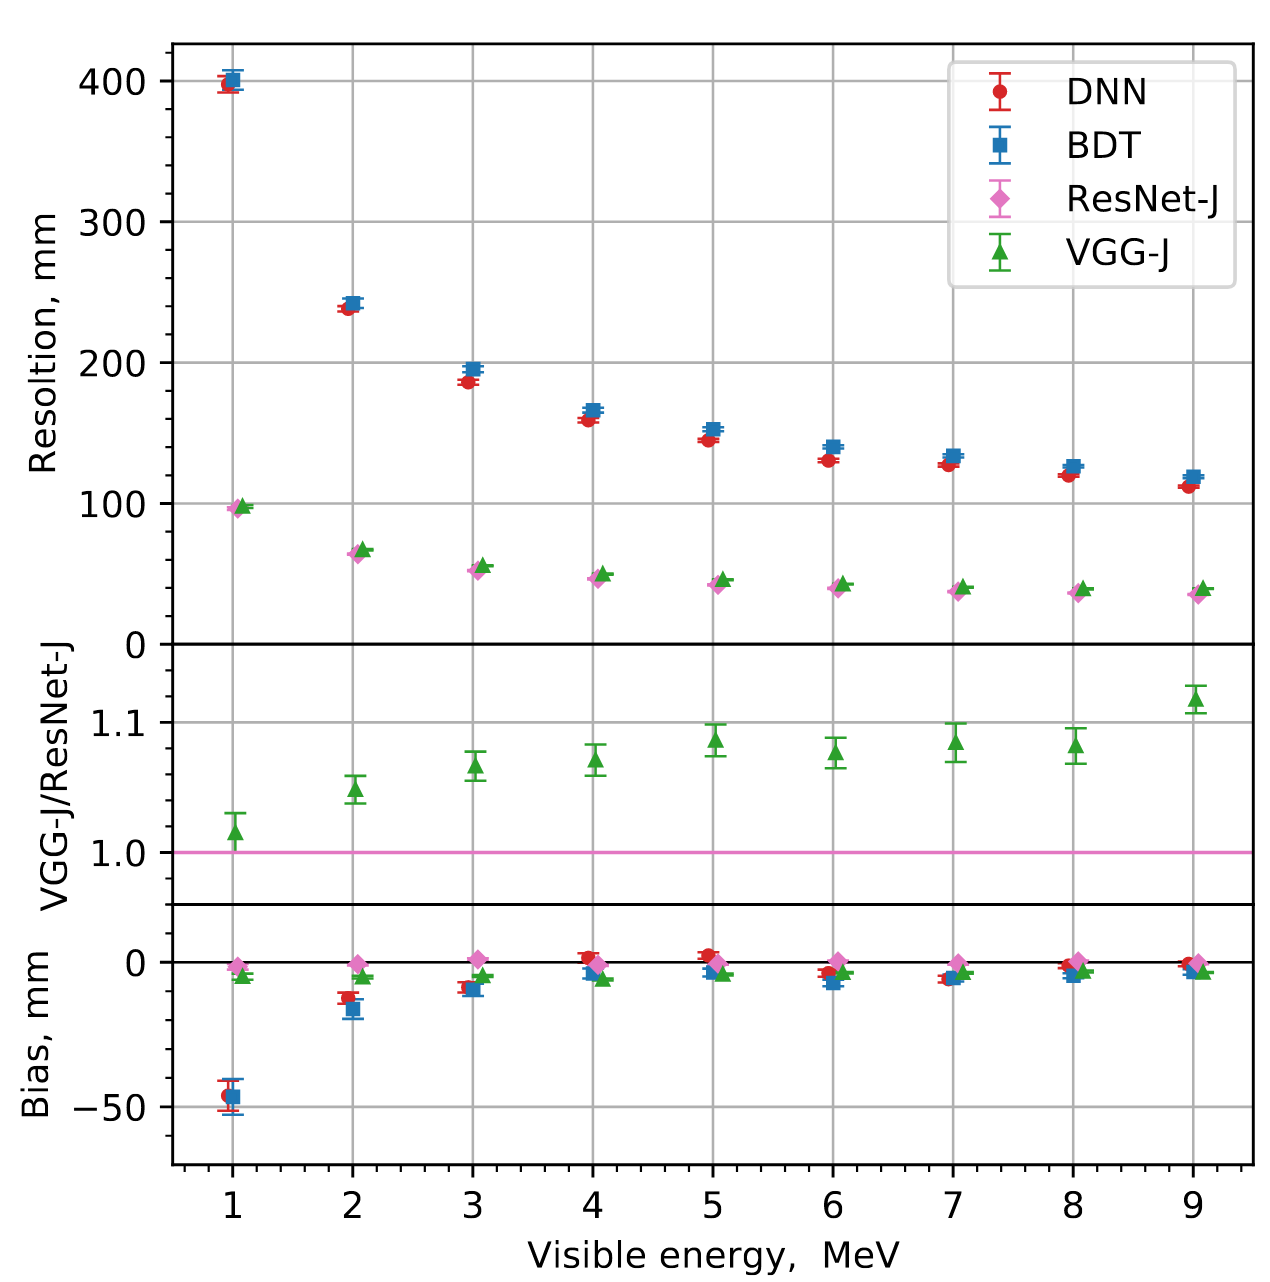
\includegraphics[width=\linewidth]{images/juno/reco/ml_vertex.png}
  \end{subfigure}
  \hfill
  \begin{subfigure}{0.48\linewidth}
    \centering
    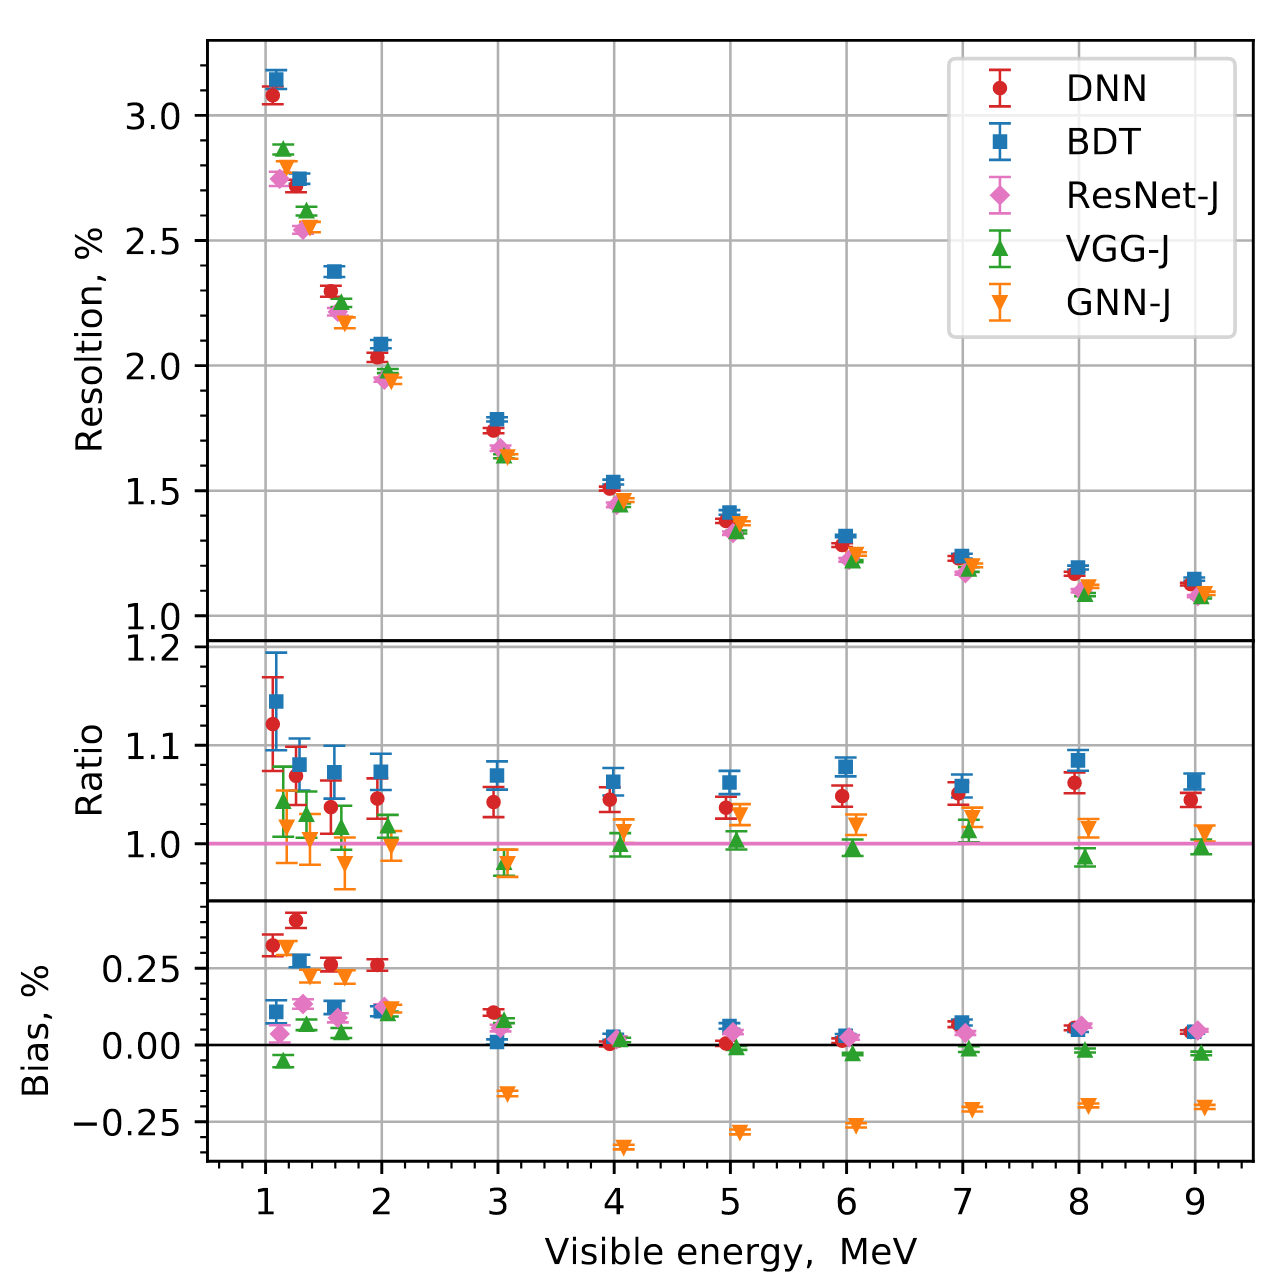
\includegraphics[width=\linewidth]{images/juno/reco/ml_energy.png}
  \end{subfigure}
  \caption{Radial (left) and energy (right) resolutions of different ML algorithms. The results presented here are from \cite{qian_vertex_2021}. DNN is a deep neural network, BDT is a BDT, ResNet-J and VGG-J are CNN and GNN-J is a GNN.}
  \label{fig:juno:rec:ml_res}
\end{figure}

Overall ML algorithms show similar performances as classical algorithms in term of energy reconstructions with the more complex structure CNN and GNN showing better performances than BDT and DNN. For vertex reconstruction, the BDT and DNN show poor performance while CNN are on the level of the classical algorithms.

\section{Conclusion}

That these first DL algorithms tried at JUNO to reconstruct IBDs do not outperform the classical method can be explained. They constitute a first exploration of these methods potential, as do the orginal GNN we describe in Chapter \ref{sec:jgnn}. Indeed, the likelihood method is also based on the full list of the charges ($Q$) and times ($t$) all PMTs, and the PDF's design accounts for an advanced knowledge of the detector (with a lot of human expertise). The fact that the methods presented in this chapter can learn enough from just the $Q,t$ list, to reach similar performance, is already an interesting result. But this is not decisive yet, in my opinion.

Actually, is there hope that one day DL methods reach better results at JUNO than classical's ? This is not a trivial question. A possibilty would be to let them start from an even rawer level (involving a number of variables which would make a likelihood intractable). This would mean, instead of $Q$ and $t$, the full waveform in each PMT. With such a quantity of input information to analyse to identify patterns, even DL methods can be limited. The choice of architecture is then important, to guide the algorithm towards pertinent features. We doubt whether CNN's would be the best choice here. We bet that GNN's could be better tools, with more flexibility to hierarchise information (the choice of which PMTs to link already helps here, as well as the possible usage of higher order quantities). The first GNN developped in JUNO (decribed above, \cite{qian_vertex_2021}) does not do that. It's still only based on $(Q,t)$ couples and link only neighbour PMTs in its first layer. It serves essentially as a way to avoid the problems encountered by CNNs due to the planar projection of a spherical image.

In chapter \ref{sec:jgnn}, we tried an original GNN architecture. The goal was not yet to include a rawer information, but to see if this architecture would perform as well as the one described above when using $Q$'s and $t$'s as the rawest information. If so, then there is hope that when rawer information will be included, this orginal architecture will be the one able to best use it.

\end{document}


\chapter{Image recognition for IBD reconstruction with the SPMT system}

\chapter{Graph representation of JUNO for IBD reconstruction with the LPMT system}

\chapter{Reliability of machine learning methods}

\chapter{Discrimination of e+/e- events in JUNO}

\chapter{Conclusion}

\printbibliography[heading=bibintoc]

\end{document}
